%duvida 1: qual melhor pessoa para usar em frazes
%   nessa etapa precisamos (ingles)
%   nessa etapa é preciso
%   nessa etapa precisei
%   nessa etapa foi necessário       usar essa

%Conjunto de equações, recomendação do emílio
%\begin{align}
%    A \in Z^{2} \\
%    mix(A, B, c) &= (1-c) * A + c*B \\
%    mix(A, B, c) &= (1-c) * A + c*B \\
%\end{align}

\chapter{Implementação}

\section{Configuração do Ambiente}
%DEBUG: Essa seção não é muito relevante para o resultado final, não sei se escrevo ela
%falar sobre implementação do sistema de navegação

\subsection{Usando os Buffers do OpenGL e GLSL}
%DEBUG: Mover para fundamentação teórica?

\subsubsection{Descrição dos vértices}
Um vértice $v$ é um conjunto de informações relacionadas a alguma unidade, %DEBUG: trocar o termo unidade
a informação necessária para este projeto é posição no espaço, então cada vértice
vai possuir uma posição notada por $v.pos$, e $v.pos$ é composto por 
$\{x, y, z\} \in \mathbb{Q}^3$. Um segundo dado será usado, a cor, vai ser uma 
informação auxiliar, usada para melhor vizialização dos resultados, 
representada por $\{r, g, b \in \mathbb{Q}:0 \leq r, g, b \leq 1\}$ onde cada um desses
vai referir a proporção de vermelho, verde e azul respectivamente.

\subsubsection{Implementação do sistema de Navegação}

\section{\textit{Terrain chunk}}
Representando um fragmento do terreno, o objeto \textit{Terrain chunk} é responsavel
por gerar uma malha para o terreno com $k^2$ vértices, o construtor pode receber 
a seguinte tupla para inicialização: 
$terrainChunk(seed, \Delta{v}, k, x_{s}, z_{s}, b, l)$
%referenciar as fatias do fernando
\begin{itemize}
    \item $seed \in \mathbb{N}$ representa a semente para começar o motor de números
    pseudo-aleatórios;
    \item $\Delta{v} \in \mathbb{Q}:0 < \Delta{v} < l/2$ é a distância entre vértices adjeacentes na
    projeção do plano $X \times Z$;
    \item $k \in \mathbb{N}>4$ é a quantidade de vértices em cada coluna ou 
    linha, a malha tem $k^2$ vértices;
    \item $x_{s} \in \mathbb{Q}:$ é o valor inicial no eixo $X$;
    \item $z_{s} \in \mathbb{Q}:$ é o valor inicial no eixo $Z$;
    \item $b \in \mathbb{N}>4:$ a área da região de cada bioma vai ser $b^2$;
    \item $l \in \mathbb{N}:1 < l < b/2$ distância para fronteira entre biomas ser interpolada.
\end{itemize}


Em cada execução da iplementação os valores que podem mudar de uma chunk para 
outra são apenas $x_{s}$ e $z_{s}$. Uma maneira de conseguir gerar terreno sobre demanda
é usando a localização da camera $(x_{c}, y_{c}, z_{c})$, quando ela se
aproxima de alguma borda da chunk atual
uma \textit{thread} é acionada pedidndo para calcular uma nova chunk, com os parâmetros
$x_{s} = x_{c}/\Delta{v} - k/2$ e $z_{s} = z_{c}/\Delta{v} - k/2$, assim que ela
estiver calculada a mesma começa a ser renderizada, substituindo a chunk anterior.
Antes de renderizar alguma chunk é necessário fazer uma translação com o vetor direção 
$(x_{s} \cdot \Delta{v}, 0.0, z_{s} \cdot \Delta{v})$, já que internamente cada chunk vai 
da posição $(0, 0)$ até $(\Delta{v} \cdot (k-1), \Delta{v} \cdot (k-1))$, mas representando a área 
no mundo $(x_{s}, z_{s})$ até $(x_{s} + \Delta{v} \cdot (k-1), z_{s} + \Delta{v} \cdot (k-1))$

\section{Criando Malha de Triângulos}
A maneira que um jogo renderiza seu terreno no final das contas é sobre uma
malha, uma malha é um conjunto de vértices que podem representar fragmentos
de uma superfície do terreno.

Para representar um segmento de plano precisamos de pelo menos $3$ vértices, 
já que com dois podemos apenas representar segmentos de retas. Um plano precisar
ter um mesmo vetor normal para todo o plano.

A malha segue pelo plano $X \times Z$, e cada vértice do plano vai ter uma altura
$y$ definida mais tarde por ruído. Se quisermos que o conjunto de pontos pertença
ao memos segmento de plano precisamos que os quatro pontos respeitem a mesma
equação do plano.%colocar referêrencia da malha de triângulos

Se usarmos como plano $4$ pontos em $\mathbb{Q}^3$
\begin{equation}\label{comp_sign_inter_sem_peso_aux}
    P = \{p_{0}(0, y_{0}, 0), p_{1}(0, y_{1}, 1), p_{2}(1, y_{2}, 0), p_{3}(1, y_{3}, 1)\}
\end{equation}
Para montar a equação do plano temos $\{y_{0}, y_{1}, y_{2}\}$ como valores livres e $y_{3}$
vai depender dos valores de $\{p_{0}, p_{1}, p_{2}\}, x_{3} e z_{3}$

%Aqui vai o cálculo da equação do plano ou do vetor normal para mostrar o que
%acabei de afirmar acima
%Calculando o vetor normal associado ao plano formado por $\{v0, v1, v2\}$
%$v0v1 = (0, y1-y0, 1)$
%$v0v2 = (1, y2-y0, 0)$

mas não é isso o objetivo, já que o ruído pode retornar valores para $y_{3}$
que não respeitem a equação do plano queremos que todos os pontos tenha valores de $y$
livres, portanto, será uma malha de triângulos. Então pro conjunto de vértices
acima temos dois triângulos associados:
$T_{1} = \{p_{0}, p_{1}, p_{2}\}, T_{2} = \{p_{3}, p_{1}, p_{2}\}$, que podem ser
vizualizados na figura \ref{fig:t1t2}. 
Desta maneira temos todos os pontos com $y$ livre.

\begin{figure}[H]
    \centering
    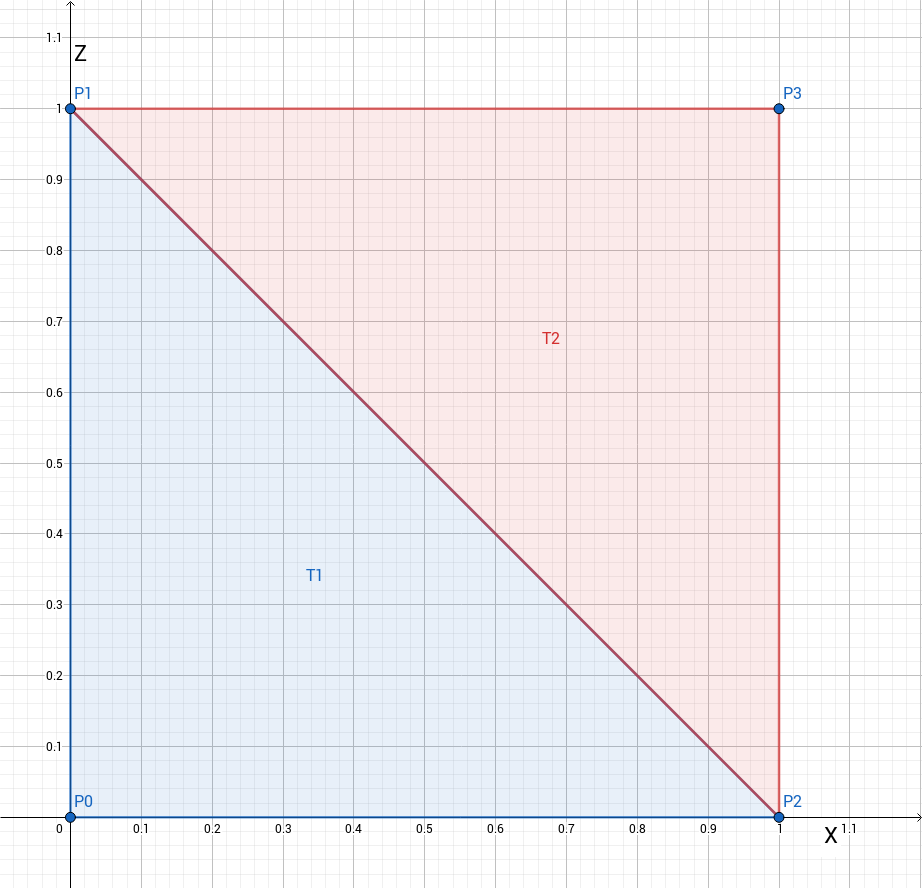
\includegraphics[width=0.5\textwidth]{figuras/t1t2.png}
    \caption{$T_{1}$ e $T_{2}$ projetados em $X \times Z$}
    \label{fig:t1t2}
\end{figure}


Então para montar um grid renderizavel usamos o algoritmo \ref{alg:genVectors}
$V$ é a estrutura que armazena os vértices, de $v_{0}$ até $v_{k^2-1}$ 
$E$ é a estrutura que armazena os índices, já que o \textit{OpenGL} precisa
saber a ordem de desenhar cada triângulo e quais vértices fazem parte dele, 
cada elemento de $e_{i} \in \mathbb{N}$ e a estrutura vai de $e_{0}$ até $e_{(k-1)^2 \cdot 6 - 1}$.

A função \textit{$hEvaluation(x, z)$}, será comentada mais adiante, ela retorna uma estrutura
com a altura e cor para algum ponto $(x, z)$.
 
\begin{algorithm}[H]\label{alg:genVectors}
    $|V| = k^2$\;
    \For{$i \leftarrow 0$ \KwTo $k-1$}{
        \For{$j \leftarrow 0$ \KwTo $k-1$}{
            $v_{i \cdot k + j}.pos \leftarrow (\Delta_{v} \cdot i, $Algoritmo\ref{alg:vertexValuationm}$(x_{s} + i, z_{s} + j).h, \Delta{v} \cdot j)$\;
            $v_{i \cdot k + j}.cor \leftarrow $Algoritmo\ref{alg:vertexValuationm}$(x_{s} + i, z_{s} + j).cor$\;
        }
    }
    $|E| = (k-1)^2 \cdot 6$\;
    \For{$i \leftarrow 0$ \KwTo $k-2$}{
        \For{$j \leftarrow 0$ \KwTo $k-2$}{
            \tcc{posições em $V$ do primeio triângulo}
            $e_{(i\cdot(k-1)+j)\cdot 6} \leftarrow (i\cdot k +j)$\;
            $e_{(i\cdot (k-1)+j)\cdot 6+1} \leftarrow (i\cdot k +j+1)$\;
            $e_{(i\cdot (k-1)+j)\cdot 6+2} \leftarrow ((i+1)\cdot k +j)$\;
            \tcc{posições em $V$ do segundo triângulo}
            $e_{(i \cdot (k-1)+j) \cdot 6+3} \leftarrow ((i+1) \cdot k +j+1)$\;
            $e_{(i \cdot (k-1)+j) \cdot 6+4} \leftarrow (i \cdot k +j+1)$\;
            $e_{(i \cdot (k-1)+j) \cdot 6+5} \leftarrow ((i+1) \cdot k +j)$\;
        }
    }
    \caption{Construção da coleção de vértices e índices.}
\end{algorithm}

Considerando que \textit{$hEvaluation(x, z)$} retorne sempre a cor branca
e a altura $0.0$, por hora os parâmetros $seed, b, l$ não terão influência, os mesmos 
só serão usados na função \textit{$hEvaluation$}, e fixando os parêmtros: $x_{s}, z_{s} = 0$, 
podemos analisar a influencia de $k$ e $\Delta_{v}$ nas figuras \ref{fig:parametrosGrid}

\begin{figure}[H]
     \centering
     \subfloat[][$k = 4, \Delta_{v} = 0.5$]{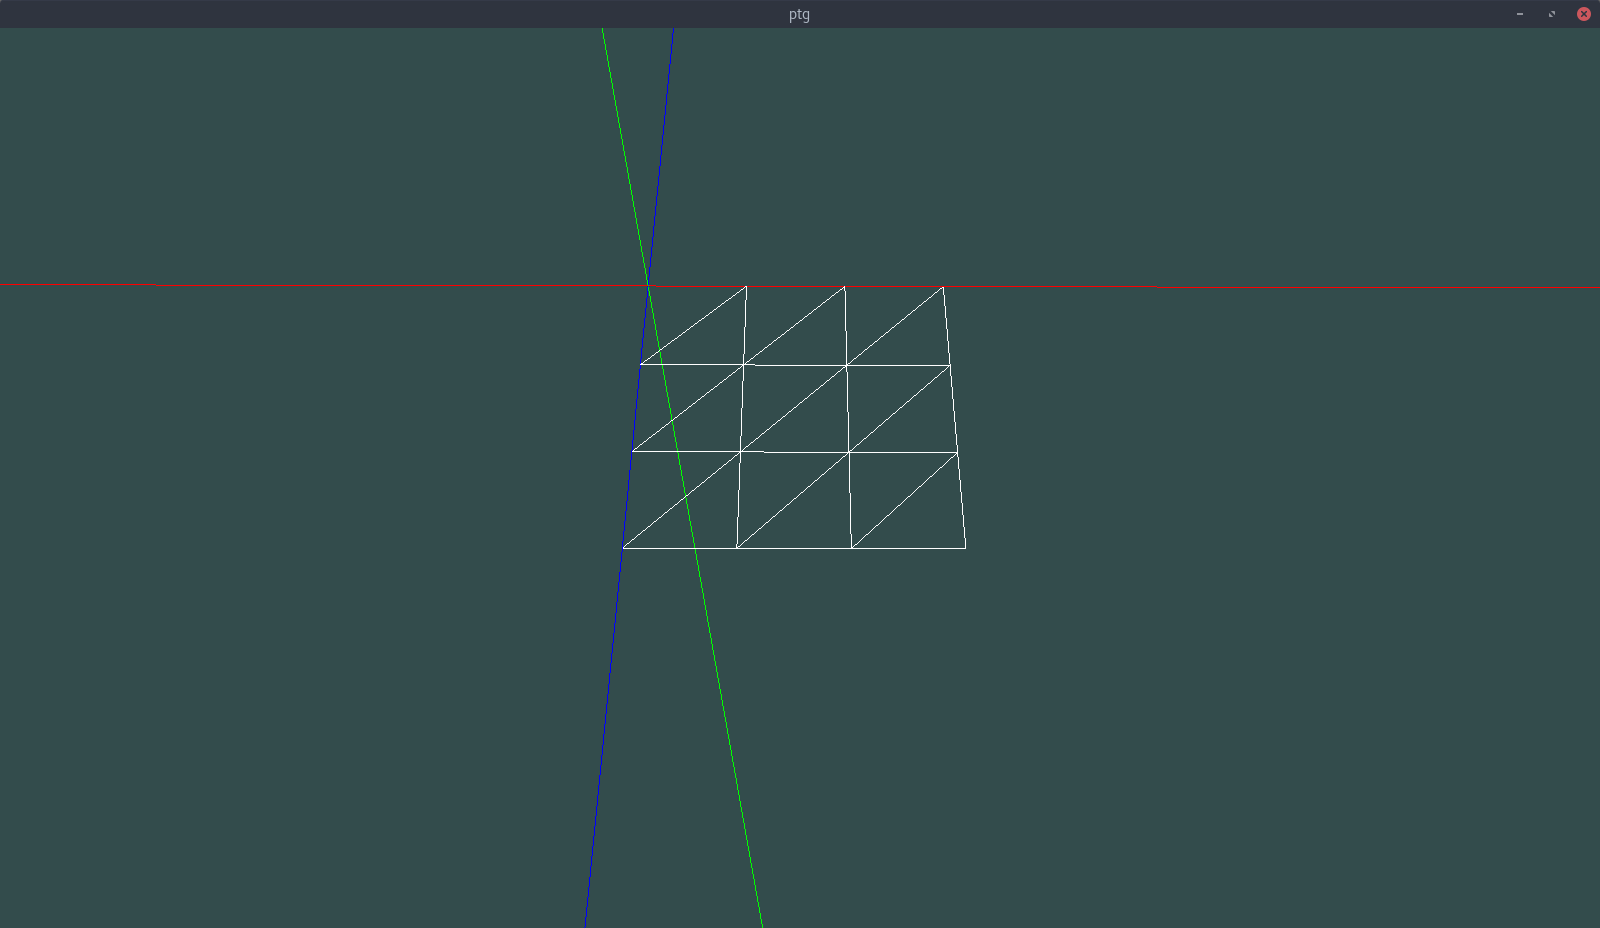
\includegraphics[width=0.3\textwidth]{figuras/k4d5.png}\label{fig:k4d5}}\hspace{0.1cm}
     \subfloat[][$k = 8, \Delta_{v} = 0.5$]{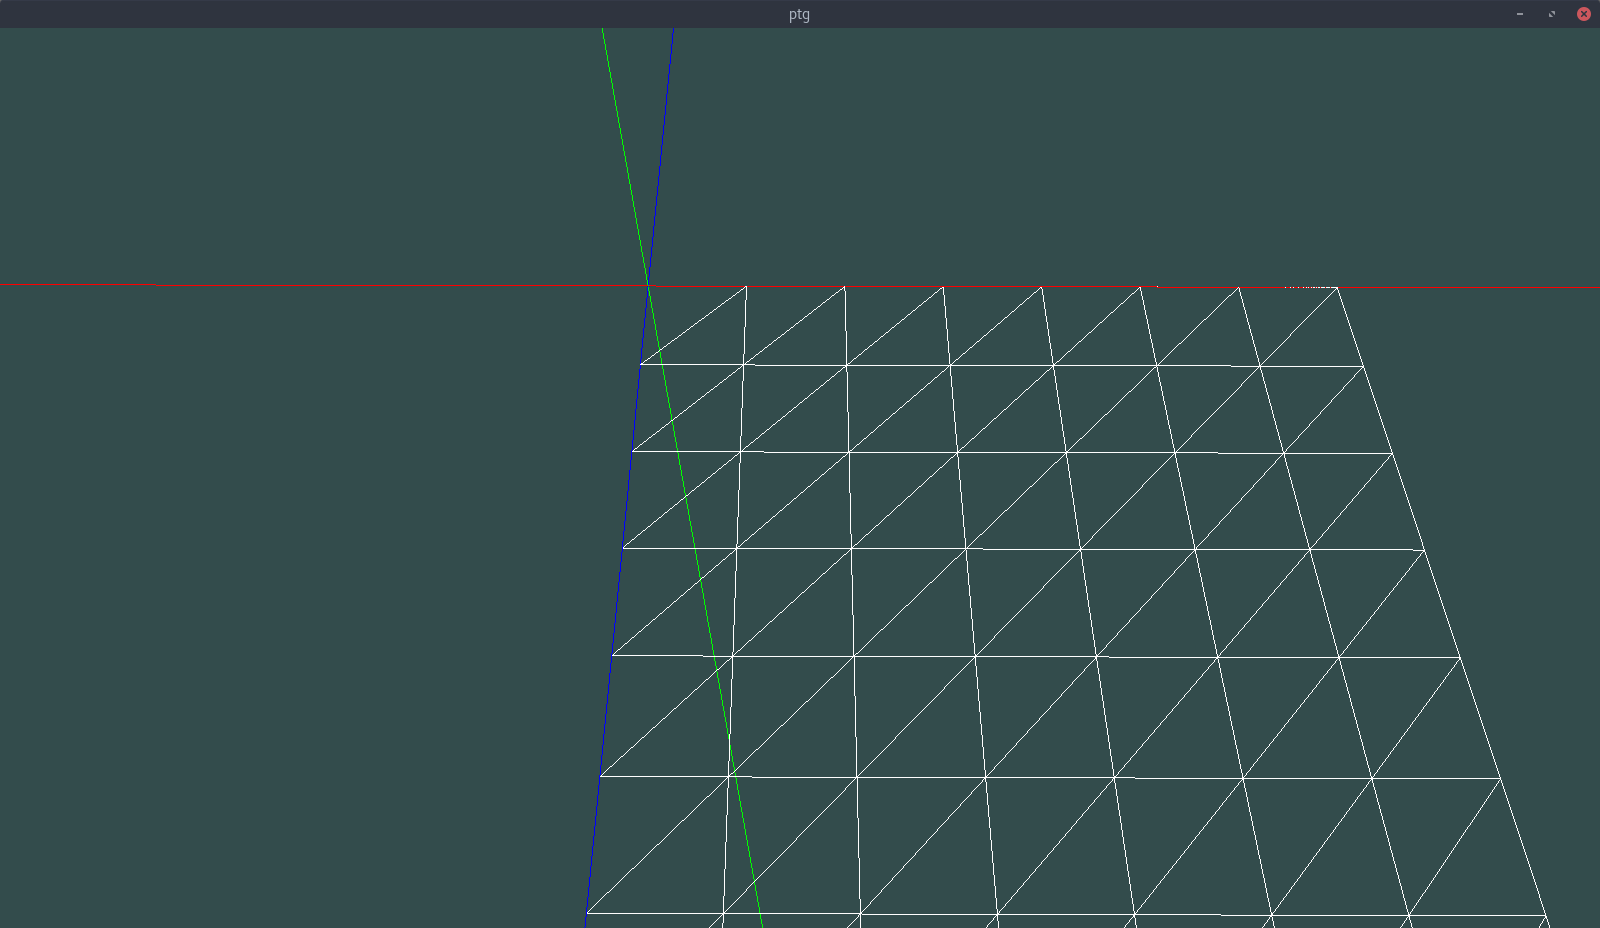
\includegraphics[width=0.3\textwidth]{figuras/k8d5.png}\label{fig:k8d5}}\hspace{0.1cm}
     \subfloat[][$k = 8, \Delta_{v} = 0.25$]{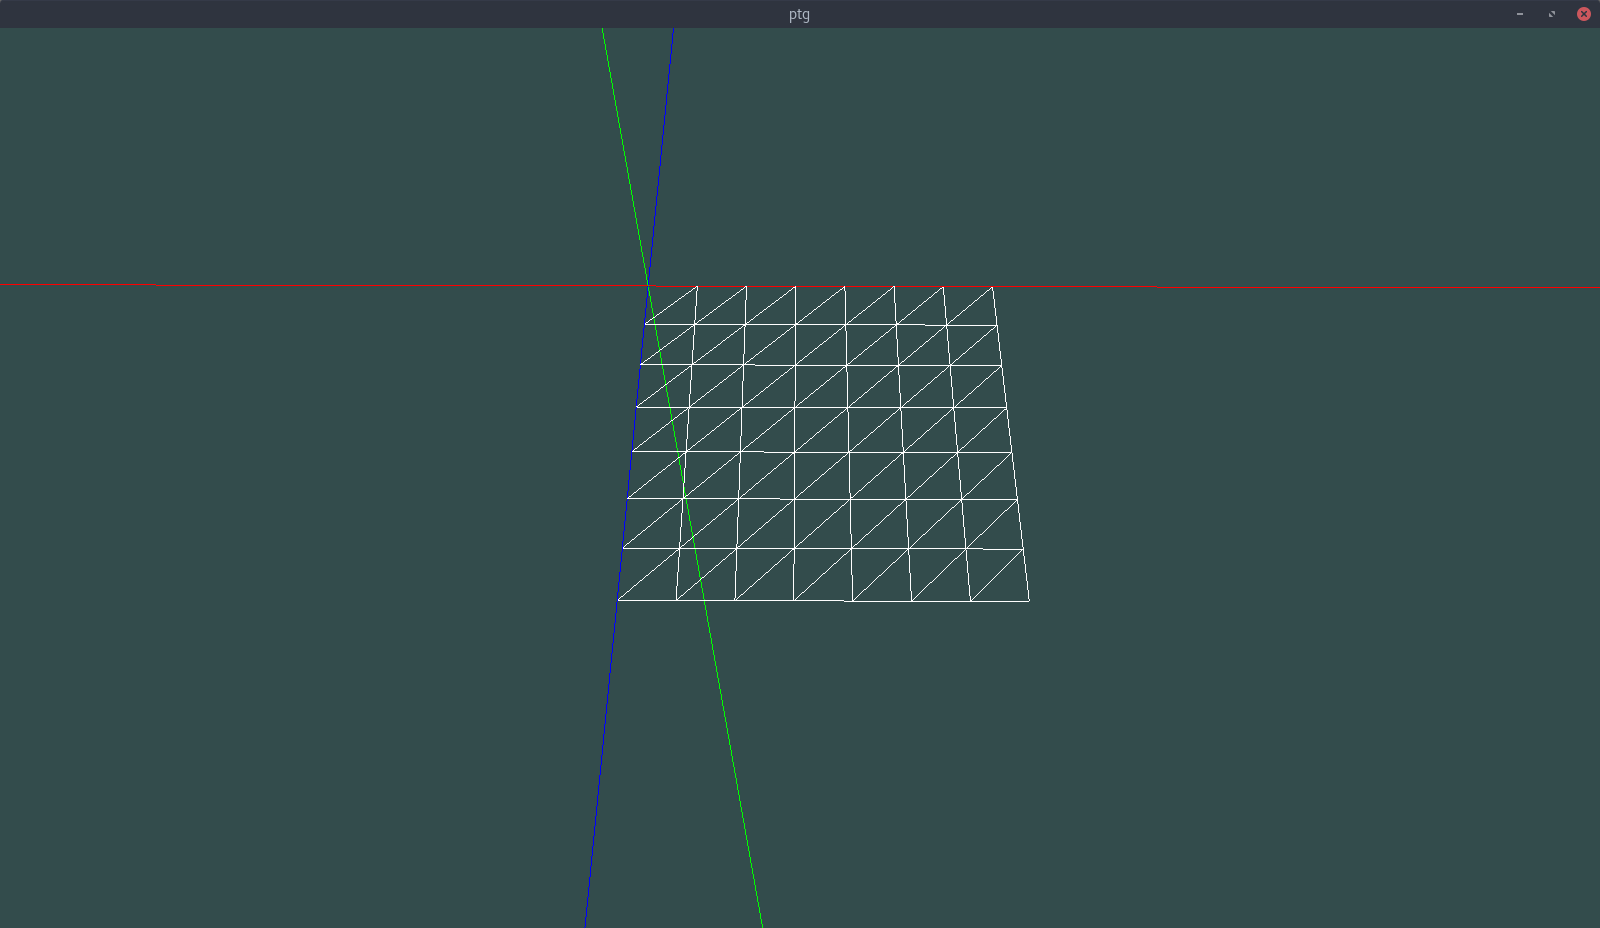
\includegraphics[width=0.3\textwidth]{figuras/k8d25.png}\label{fig:k8d25}}
     \caption{Comparando os parâmetros $k$ e $\Delta_{v}$}
     \label{fig:parametrosGrid}
     % usar \hspace{0.1cm}, é gambiarra mas funciona
\end{figure}


\section{Aplicando Ruído de Perlin nos Vértices}


\begin{figure}[H]
    \centering
    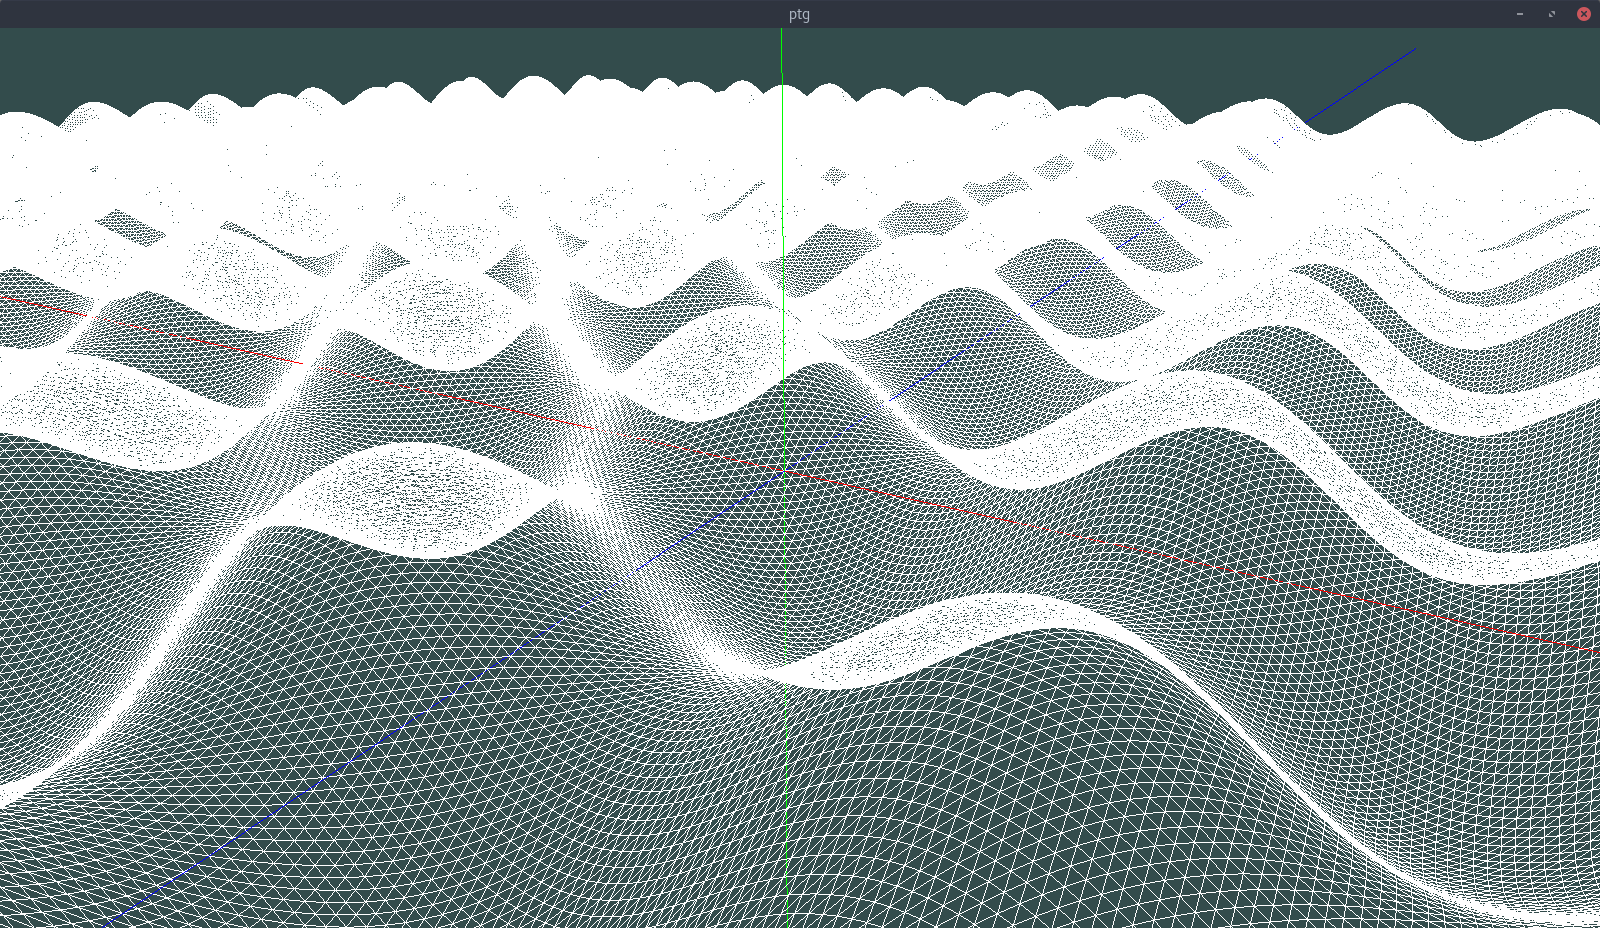
\includegraphics[width=0.75\textwidth]{figuras/sssins.png}
    \caption{Se a altura for $(sin(x/10) + sin(z/10)) \cdot 4$}
    \label{fig:sssins}
\end{figure}

DEBUG: Usando ruído de Perlin...\\
$\theta$ são as oitavas, a quantidade de vezes que um ruído será calculado 
como já explicado em perlin noise. DEBUG, fazer o que acabei de falar
$amp$ é a amplitude escalar do terreno.\\
$f$ é a frequência;\\
$fxz$ é a frequência relativa a malha;\\
$fxz = k/f$\\
$h' = PerlinNoise(x/fxz, z/fxz, \theta) \cdot amp$\\
$h = h' \cdot amp$, $h$ é valor de altura recebido pelo algoritmo \ref{alg:genVectors}, quando chama $hEvaluation(x_{s} + i, z_{s} + j).h$.

Usando $f = 8$, $amp = 30, seed = 15$ e variando o número de oitavas.

\begin{figure}[H]
     \centering
     \subfloat[][$\theta = 1$]{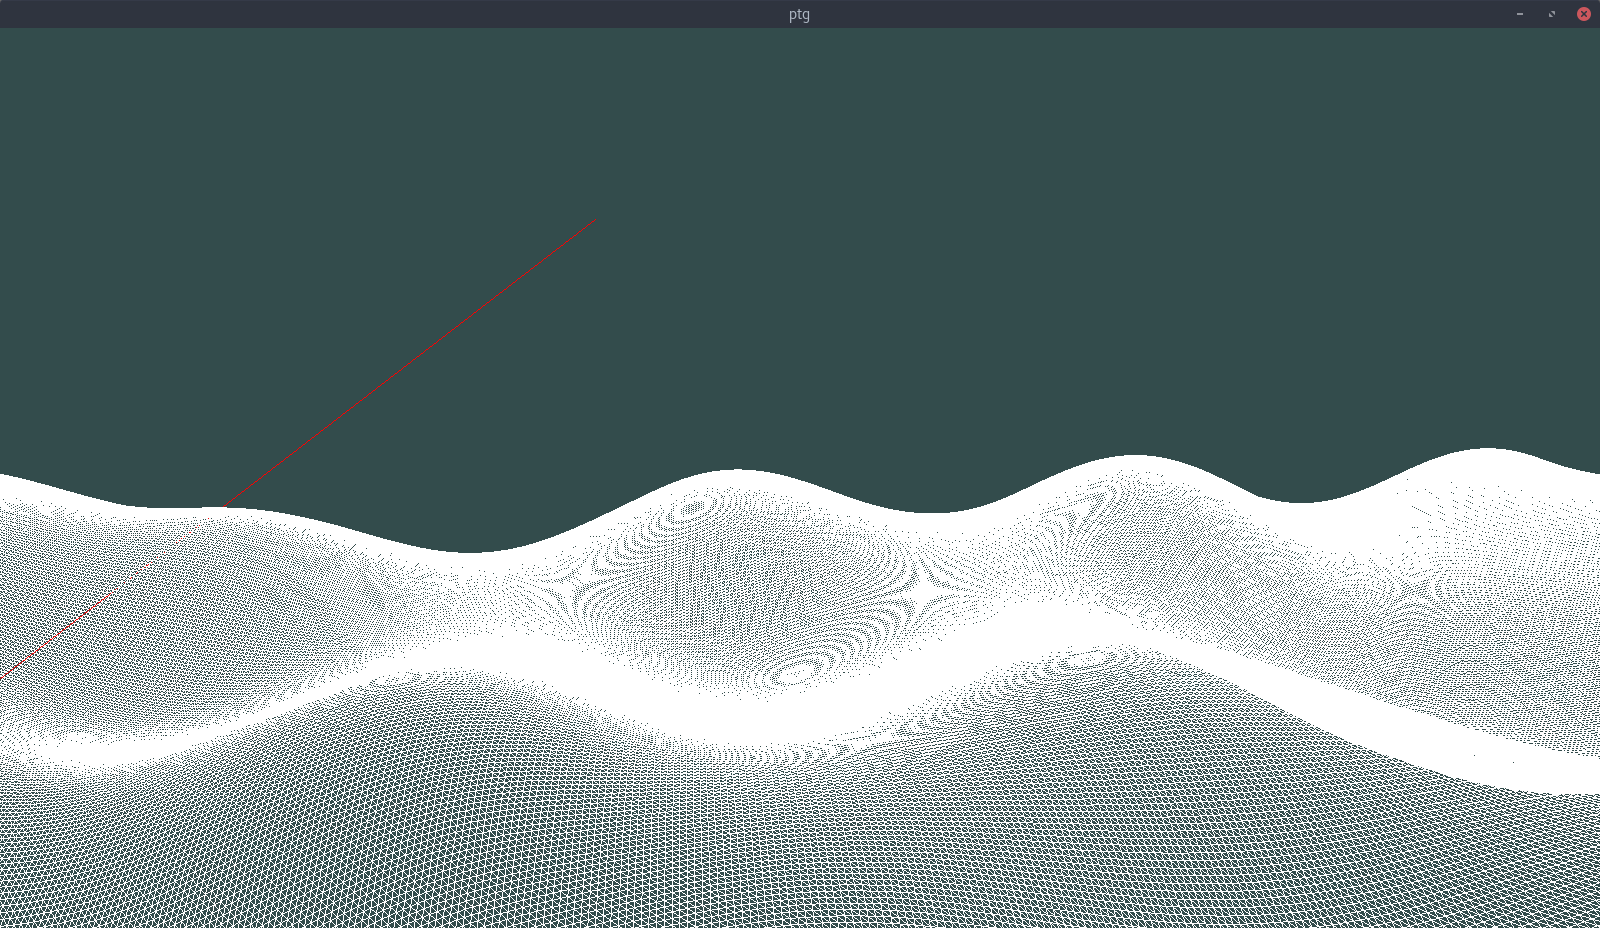
\includegraphics[width=0.3\textwidth]{figuras/octaves1.png}\label{fig:octaves1}}\hspace{0.1cm}
     \subfloat[][$\theta = 4$]{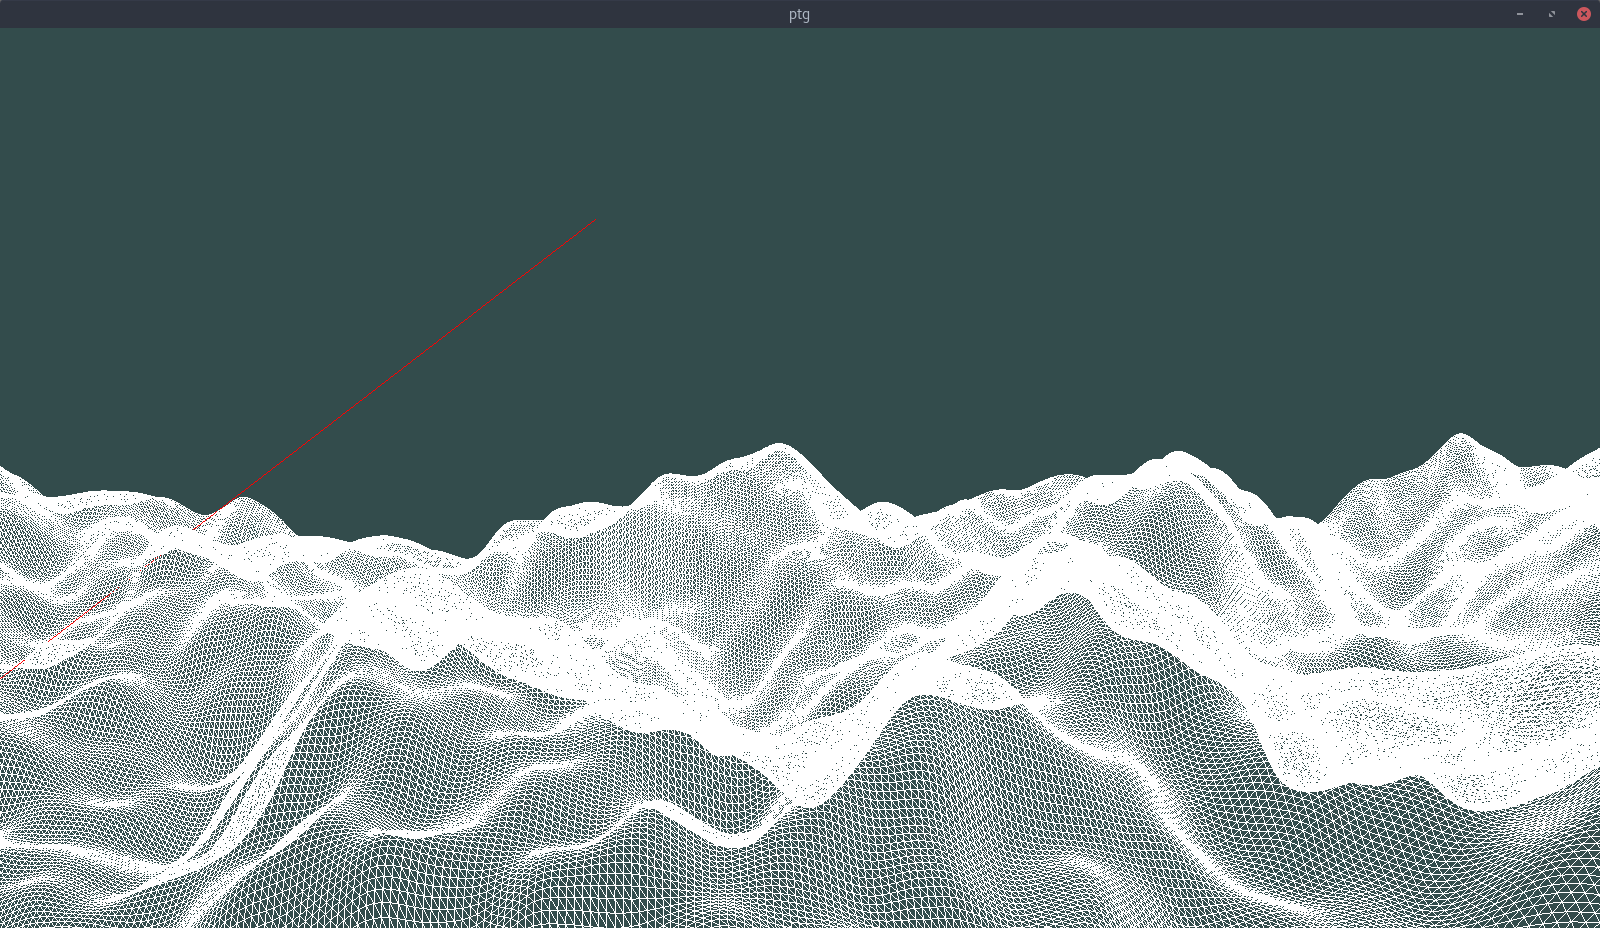
\includegraphics[width=0.3\textwidth]{figuras/octaves4.png}\label{fig:octaves4}}\hspace{0.1cm}
     \subfloat[][$\theta = 16$]{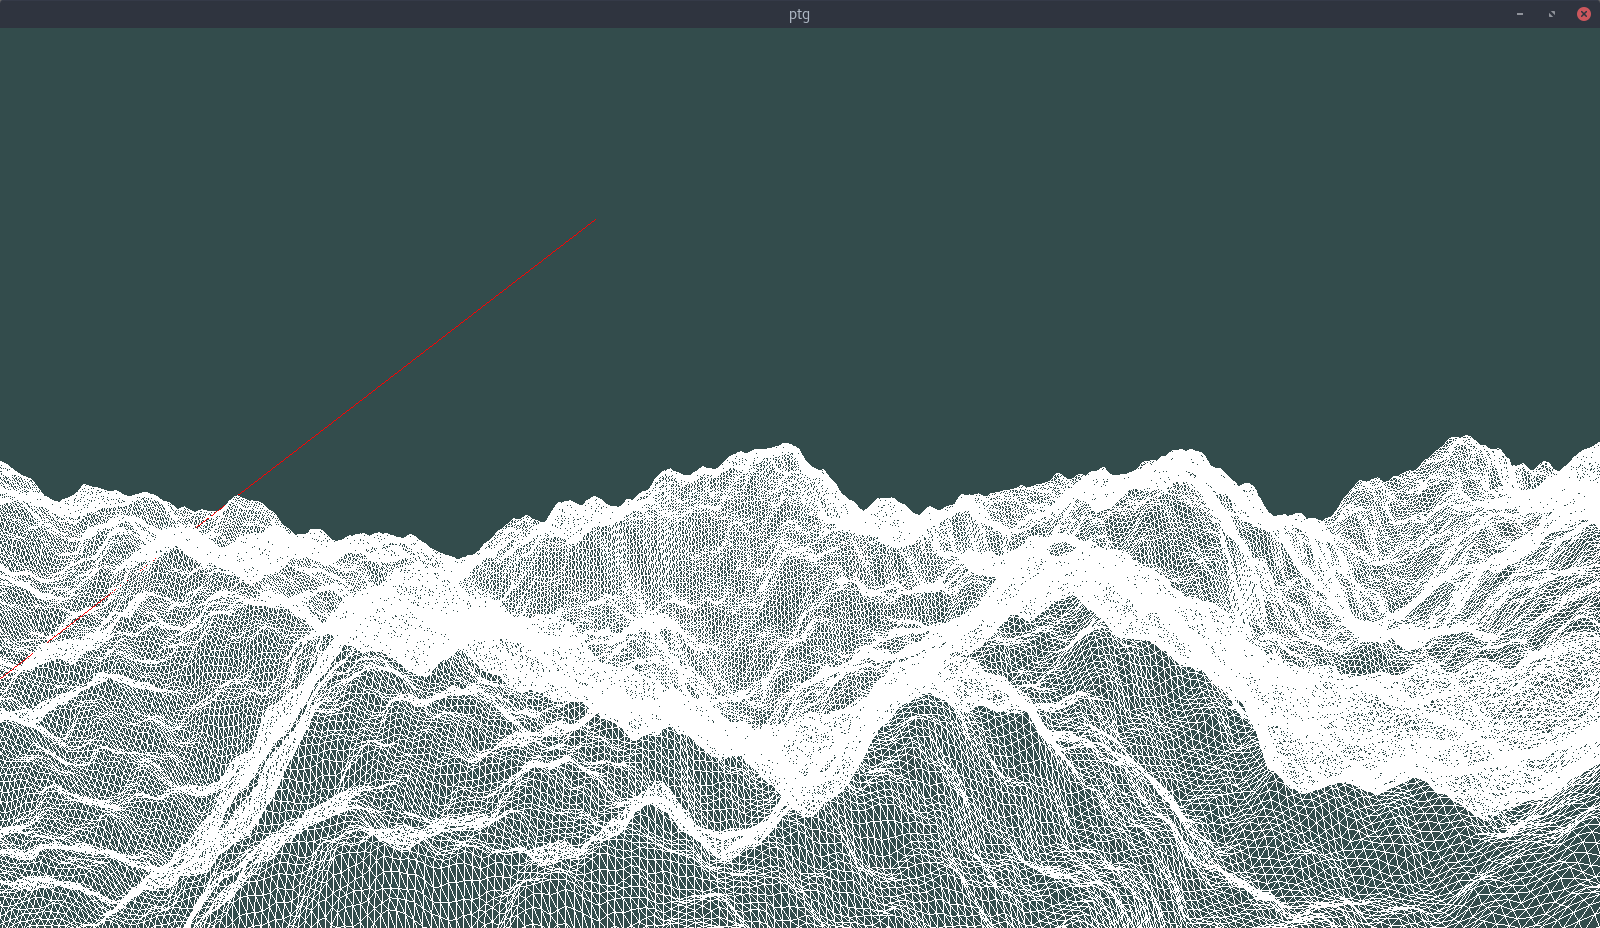
\includegraphics[width=0.3\textwidth]{figuras/octaves16.png}\label{fig:octaves16}}
     \caption{Comparando influência das oitavas.}
     \label{fig:parametrosOctaves}
     % usar \hspace{0.1cm}, é gambiarra mas funciona
\end{figure}

Usando $amp = 30$ e $\theta = 8, seed = 15$ e variando a frequência.

\begin{figure}[H]
     \centering
     \subfloat[][$f = 1$]{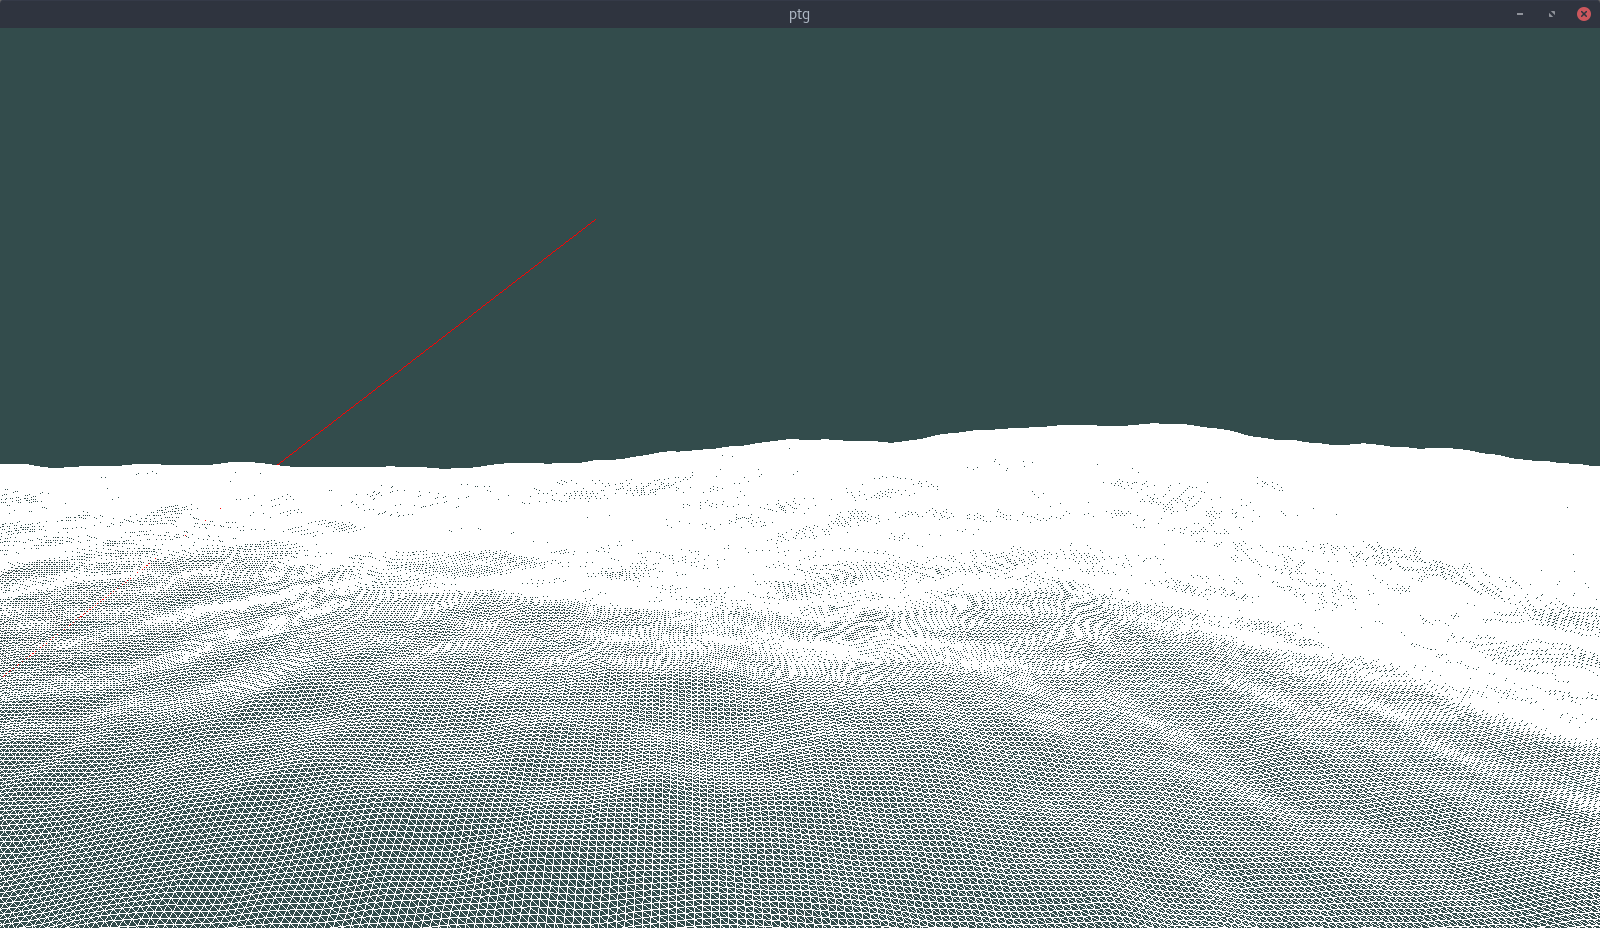
\includegraphics[width=0.3\textwidth]{figuras/freq1.png}\label{fig:freq1}}\hspace{0.1cm}
     \subfloat[][$f = 4$]{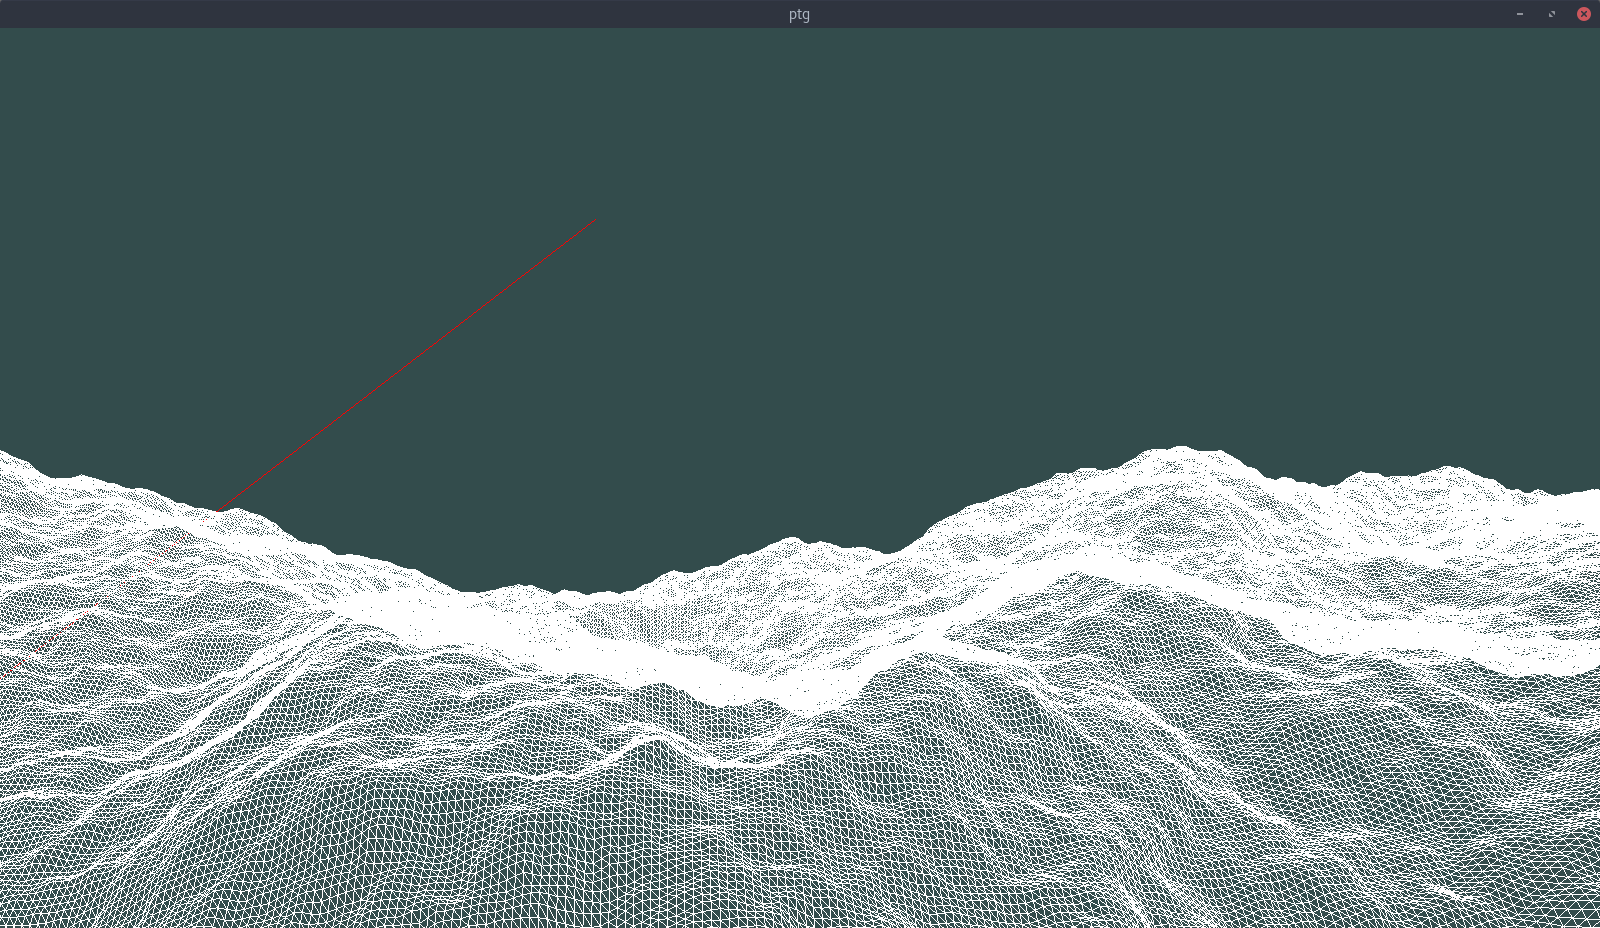
\includegraphics[width=0.3\textwidth]{figuras/freq4.png}\label{fig:freq4}}\hspace{0.1cm}
     \subfloat[][$f = 16$]{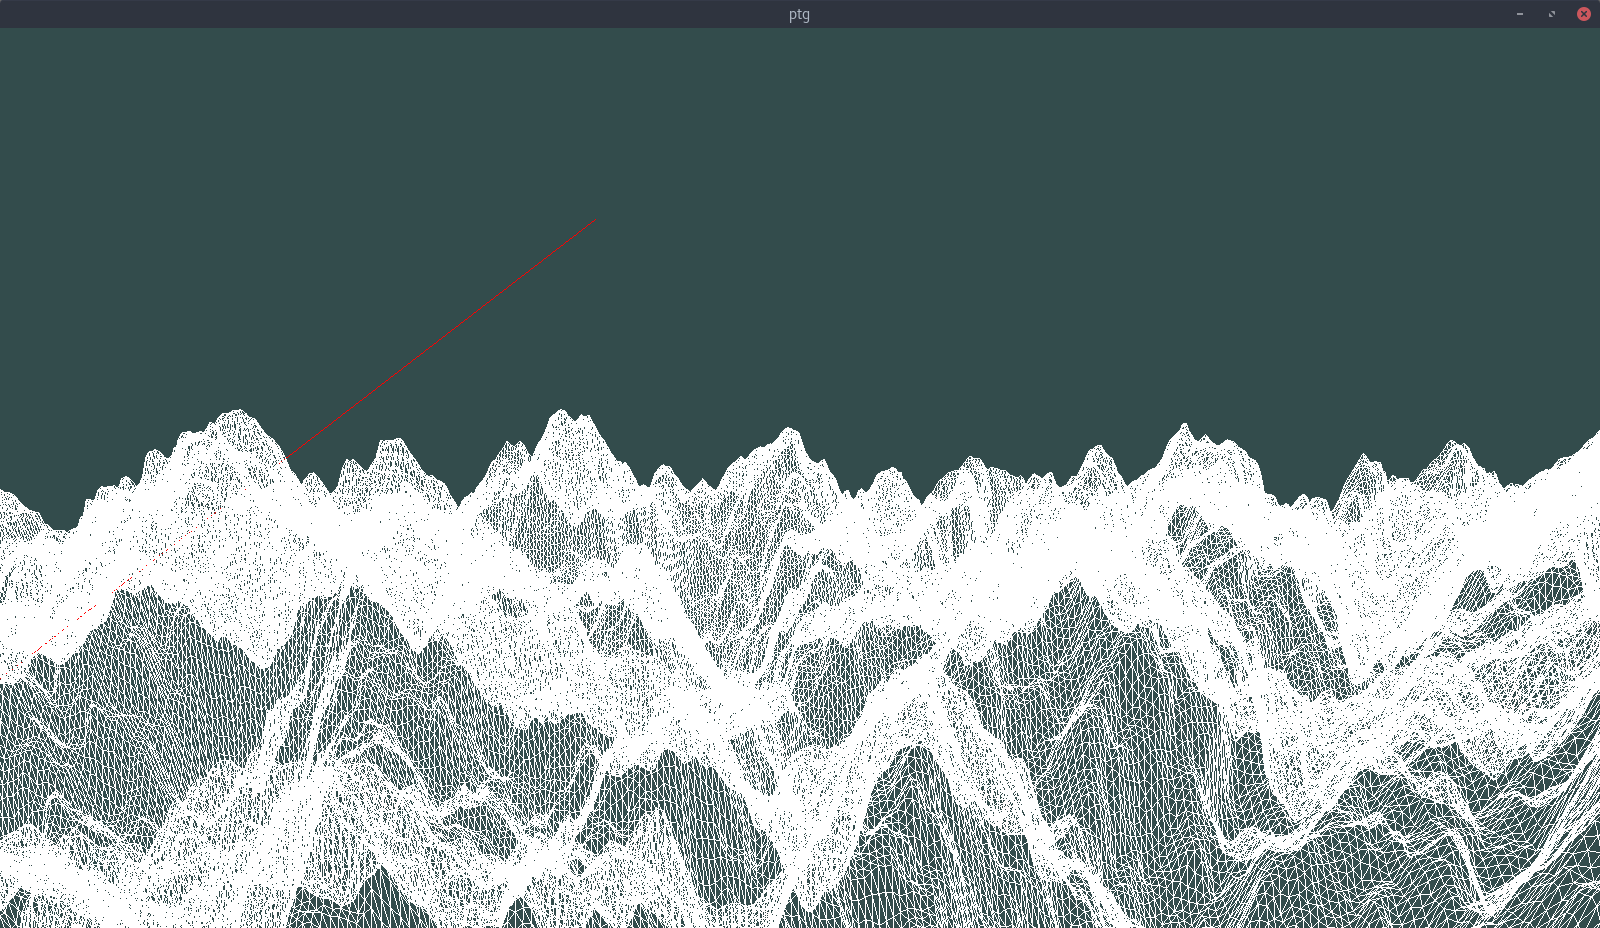
\includegraphics[width=0.3\textwidth]{figuras/freq16.png}\label{fig:freq16}}
     \caption{Comparando influência da frequência.}
     \label{fig:parametrosfreq}
     % usar \hspace{0.1cm}, é gambiarra mas funciona
\end{figure}

Usando $f = 8, amp = 30$ e $\theta = 8, seed = 15$ e variando a seed.

\begin{figure}[H]
     \centering
     \subfloat[][$seed = 1$]{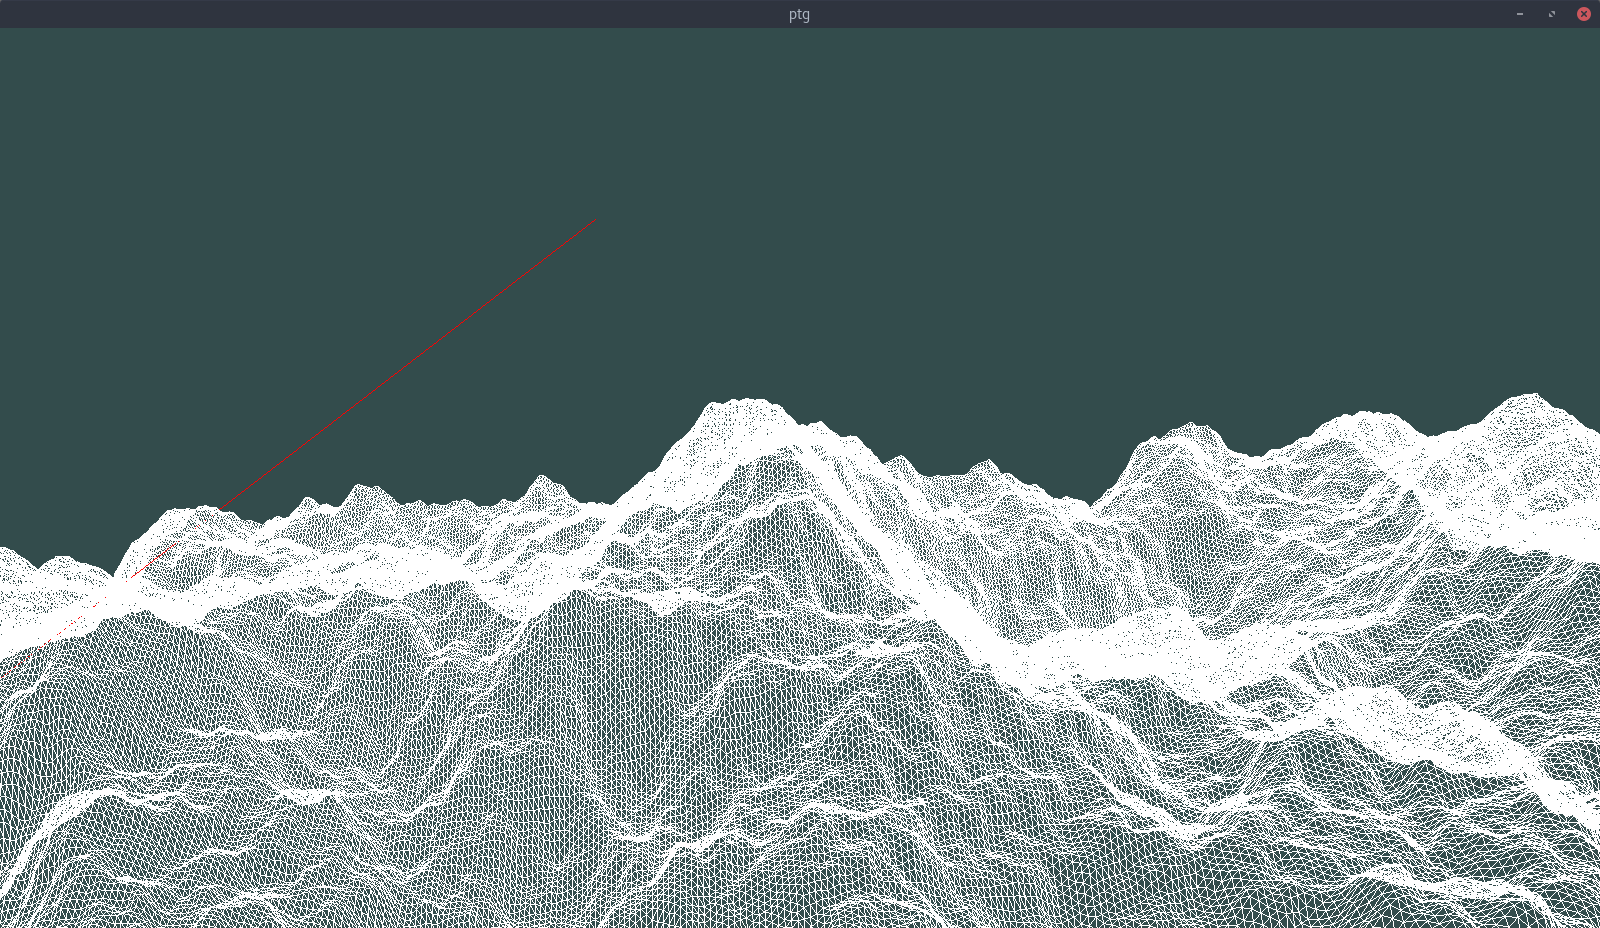
\includegraphics[width=0.3\textwidth]{figuras/seed1.png}\label{fig:seed1}}\hspace{0.1cm}
     \subfloat[][$seed = 2$]{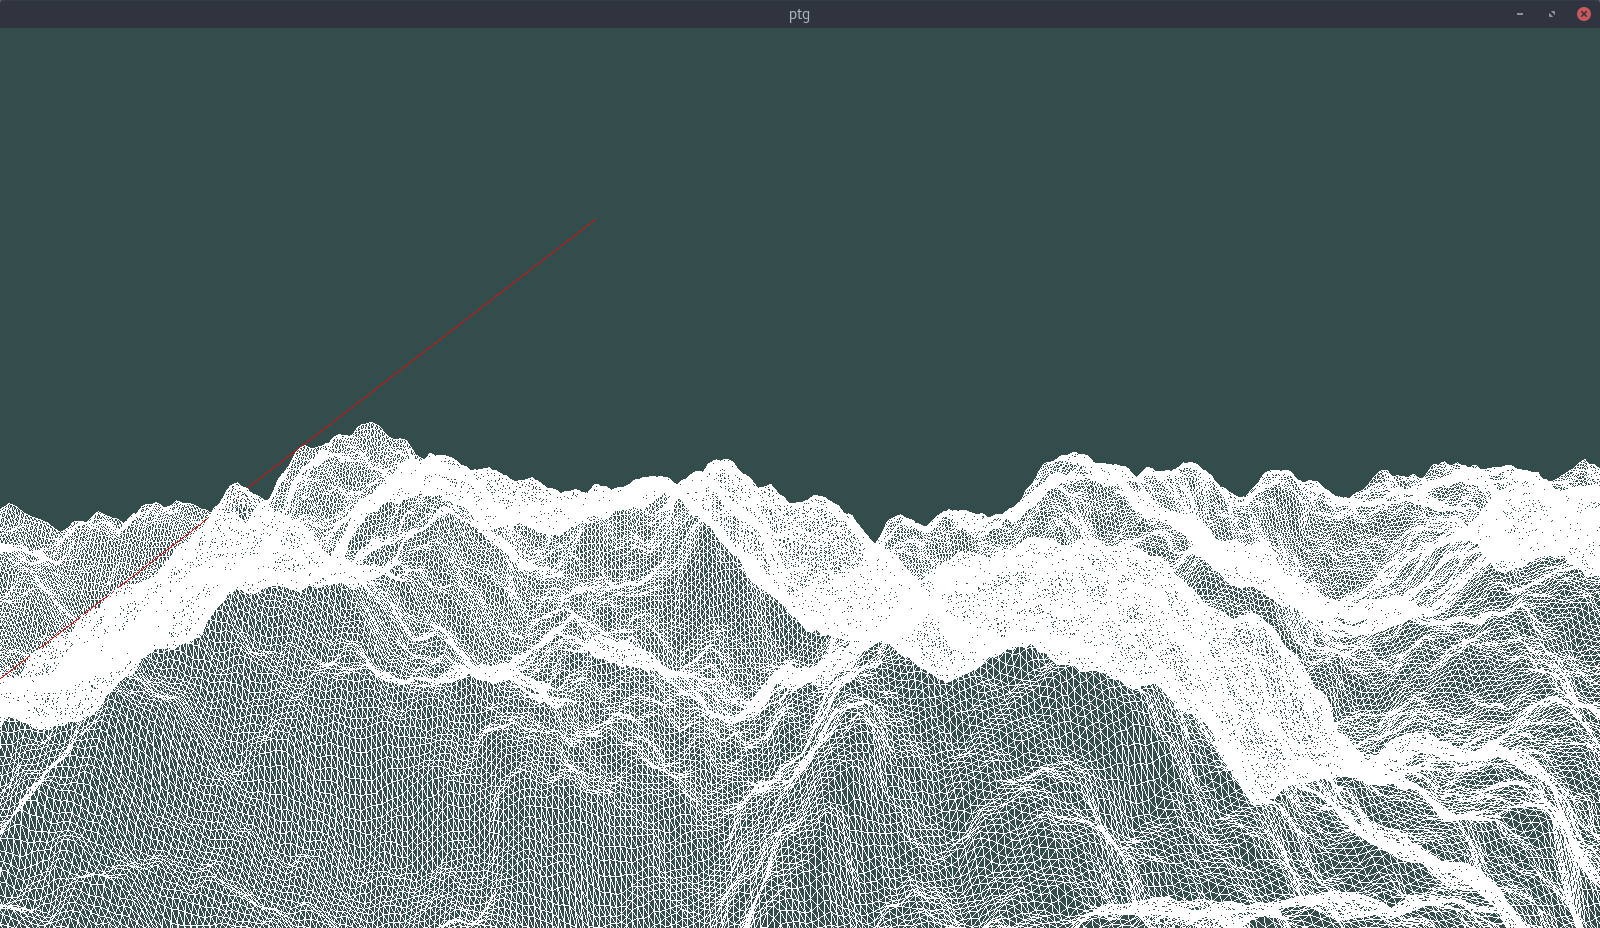
\includegraphics[width=0.3\textwidth]{figuras/seed2.png}\label{fig:seed2}}\hspace{0.1cm}
     \subfloat[][$seed = 3$]{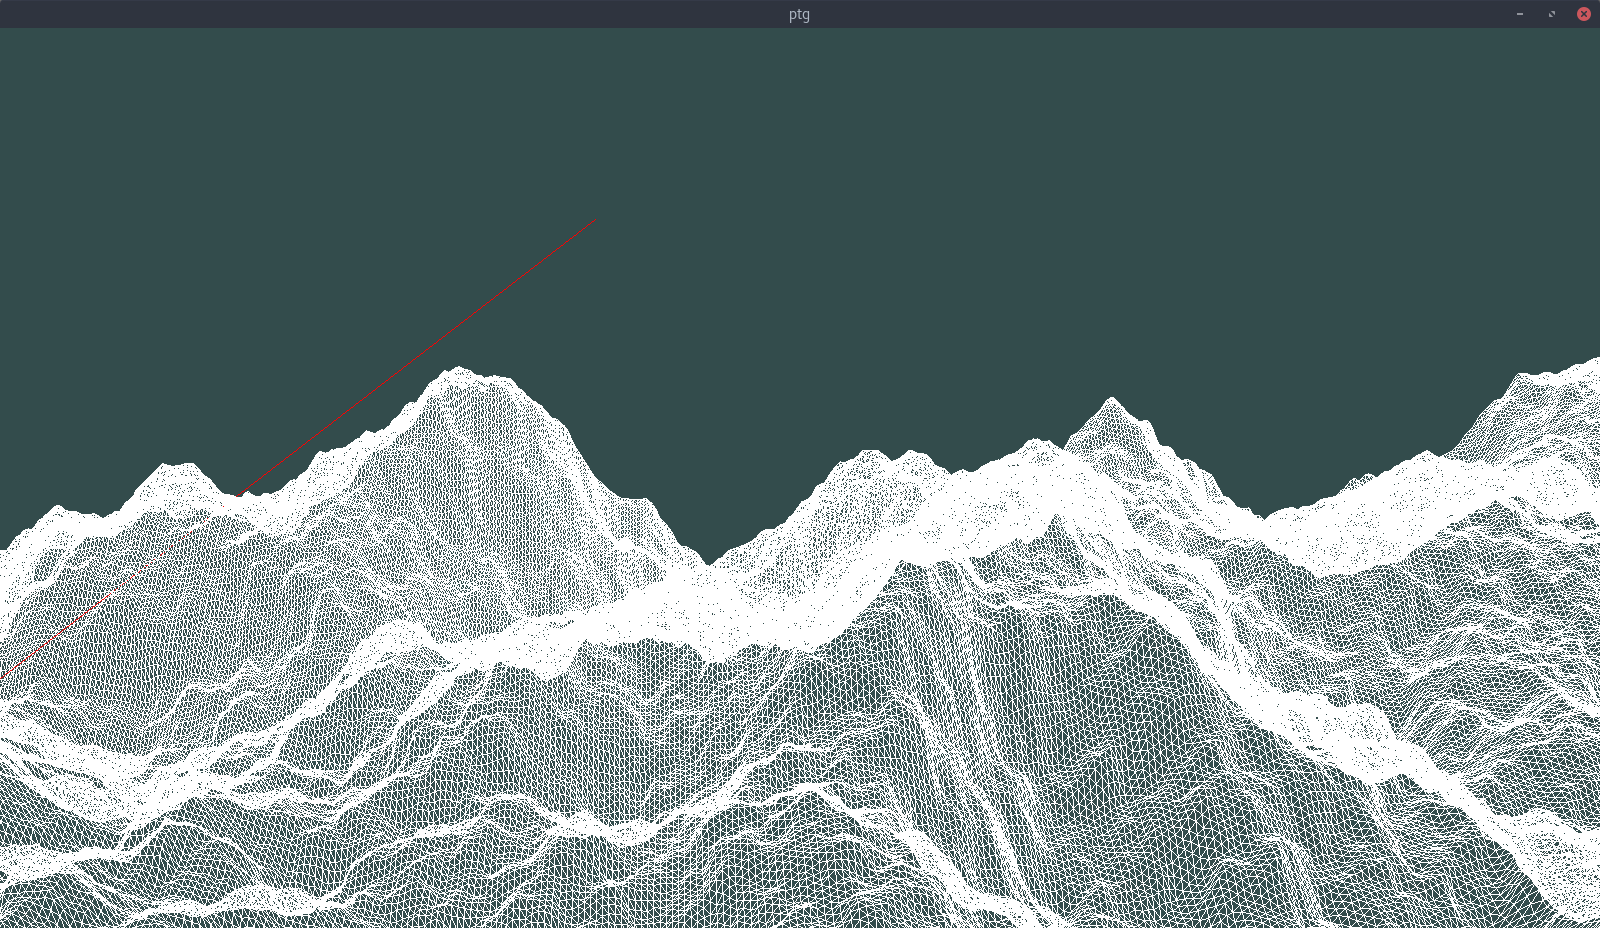
\includegraphics[width=0.3\textwidth]{figuras/seed3.png}\label{fig:seed3}}
     \caption{Comparando influência da seed.}
     \label{fig:parametrosSeed}
     % usar \hspace{0.1cm}, é gambiarra mas funciona
\end{figure}


\subsection{Cores}
Como em um jogo o terreno é representado por segmentos de planos e não um conjunto
de vértices e arestas, vamos colorir o terreno apenas para facilitar um pouco a
vizualização do mesmo. O valor $h'$ vai ficar com valores entre $-1$ e $1$, 
quando passar desse intervalo temos certeza que $-2 < h' > 2$.
%DEBUG: preciso mostrar a fómula de recorência pra isso, seria bom se a mesma já foce explicada na sessão de perlin noise.
Então podemos
usar o algoritmo \ref{alg:colorValuation} para definir a cor do vértice baseado na altura.
$cor$ no algorimo \ref{alg:colorValuation} é o valor recebido pelo algoritmo \ref{alg:genVectors}
quando chama $hEvaluation(x_{s} + i, z_{s} + j).cor$.

\begin{algorithm}[H]\label{alg:colorValuation}
    \SetKwInOut{Input}{entrada}\SetKwInOut{Output}{output}
    \Input{$minColor \in \mathbb{Q}^{3}, midColor \in \mathbb{Q}^{3}, maxColor \in \mathbb{Q}^{3}, h' \in \mathbb{Q}$}
    $auxNoise =$ clamp($h', -1, 1$)\;
    \If {$auxNoise < 0$}{
        $cor \leftarrow$ mix($midColor, minColor, auxNoise \cdot -1$)\;
    }\Else{
        $cor \leftarrow$ mix($midColor, maxColor, auxNoise$)\;
    }
    retorna $cor$\;
    \caption{Coloração de vértices.}
\end{algorithm}

Se as cores de parâmetro forem $minColor = (1, 0, 0)$(vermelho), $midColor = (0, 1, 0)$(verde) e $maxColor = (0, 0, 1)$(azul)
temos o resultado da figura \ref{fig:ssnhaha3}.

\begin{figure}[H]
     \centering
     \subfloat[][malha branca]{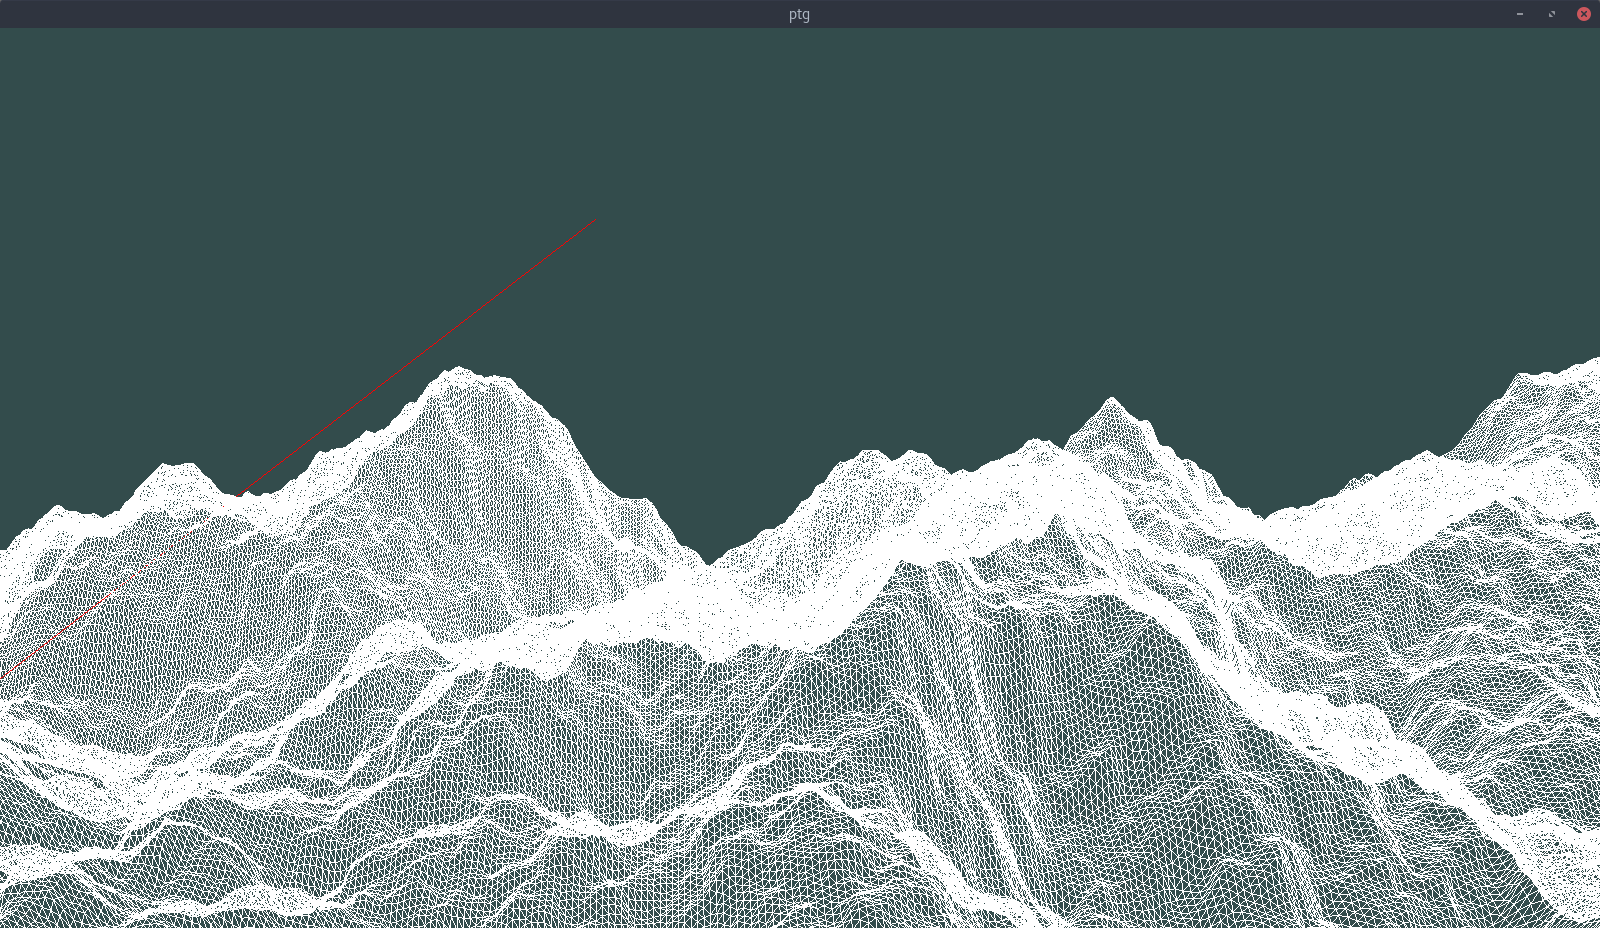
\includegraphics[width=0.65\textwidth]{figuras/ssmeshblank.png}\label{fig:ssnhaha1}}\\
     \subfloat[][segmentos de planos branco]{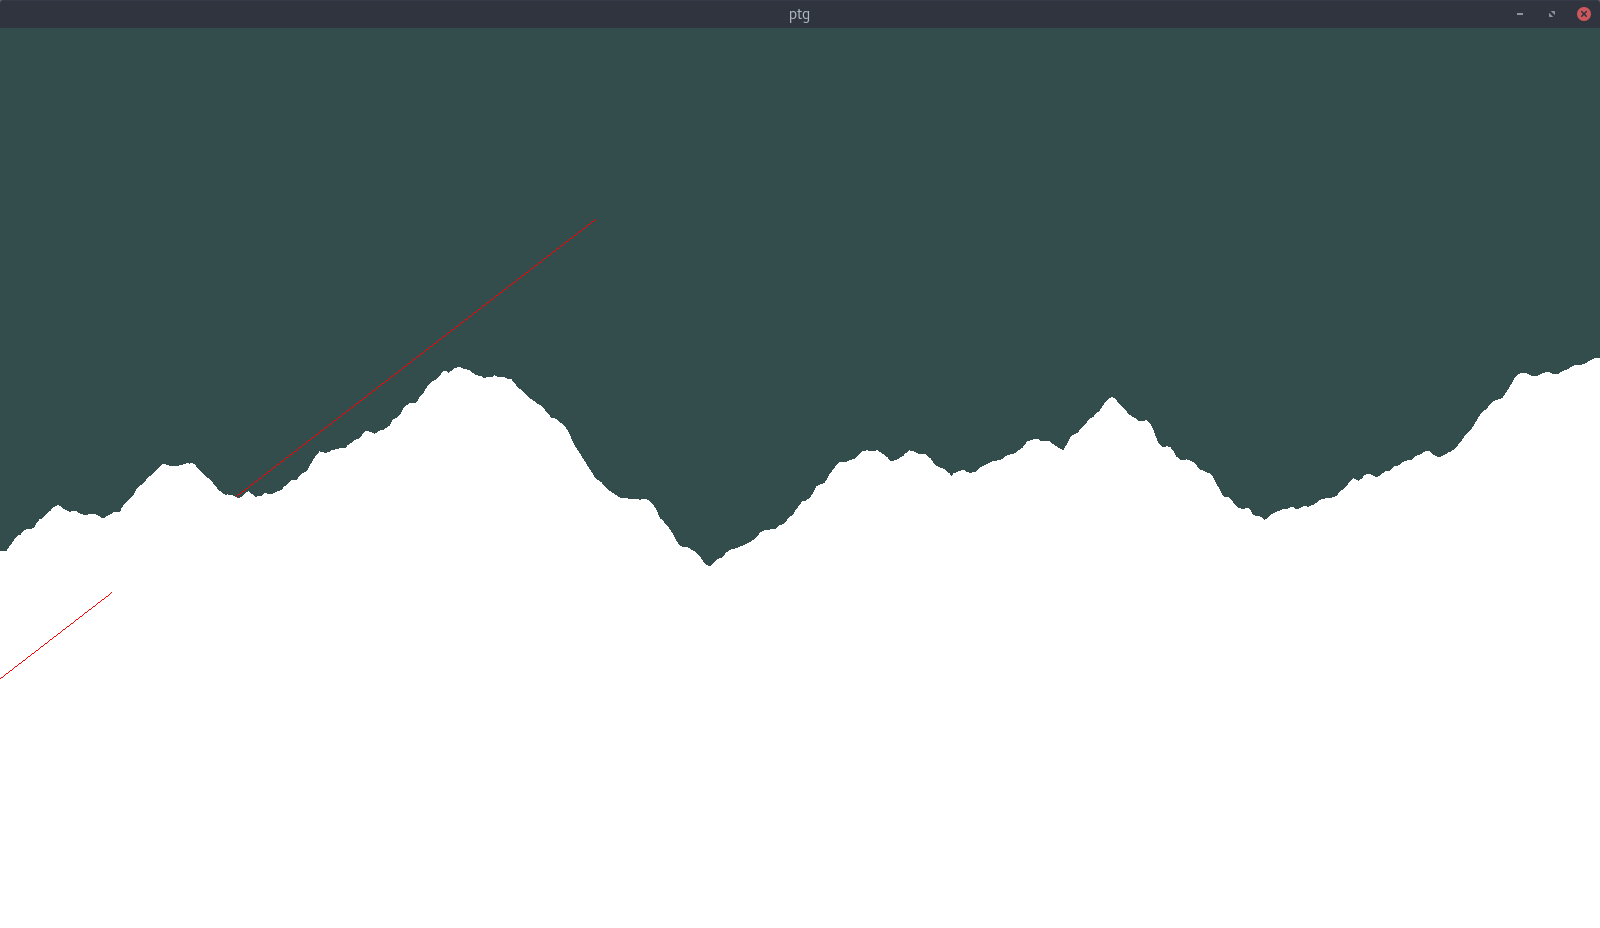
\includegraphics[width=0.45\textwidth]{figuras/ssplainblank.png}\label{fig:ssnhaha2}}\hspace{0.1cm}
     \subfloat[][segmentos de planos coloridos]{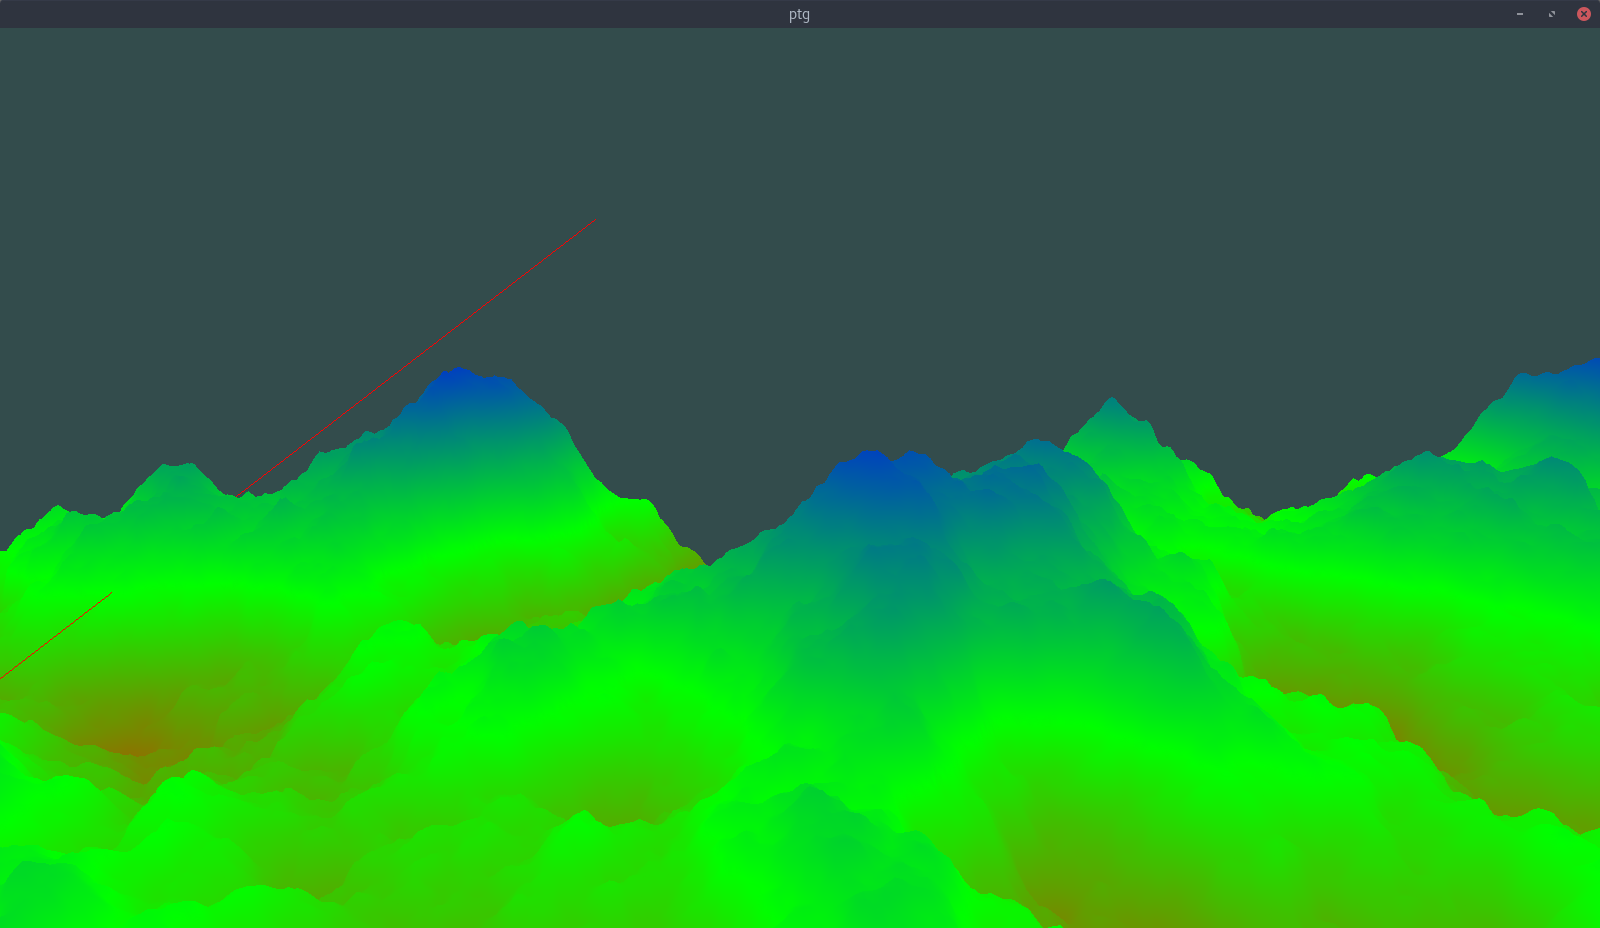
\includegraphics[width=0.45\textwidth]{figuras/ssplaincolor.png}\label{fig:ssnhaha3}}
     \caption{Usando algoritmo de coloração de vértice.}
     \label{fig:color}
     % usar \hspace{0.1cm}, é gambiarra mas funciona
\end{figure}

\subsection{Manipulando ruído para criar Biomas}
Para criar múltiplos biomas foi usado valores de cores distintas para cada um deles, 
para que quando houvesse uma fronteira entre biomas a mesma podesse ser mais notada, as
cores usadas para cada um dos biomas está na tabela \ref{tab:bioColors}.
\begin{table}[H]
    \centering
    \caption{Descrição das cores por biomas.}
    \label{tab:bioColors}
    \begin{tabular}{| c | c c c c c c|}
        \hline
        $biomaTipo$ & int id & $f$ & $\theta$ & $minColor'$ & $midColor'$ & $maxColor'$\\
        \hline
        Planícies   & 0 & $10$ & $4$ & $(34, 139, 34) $ & $(154, 205, 50) $ & $(143,188,143)  $  \\
        Montanhas & 1 & $18$ & $8$ & $(128, 128, 0) $ & $(112, 128, 144)$ & $(255, 255, 255)$  \\
        Vales   & 2 & $8$  & $8$ & $(30, 144, 255)$ & $(46, 139, 87)  $ & $(34, 139, 34)  $  \\
        Deserto   & 3 & $6$  & $2$ & $(0, 0, 0)     $ & $(244, 164, 96) $ & $(255, 255, 255)$  \\
        Cânyons  & 4 & $6$  & $4$ & $(0, 0, 0)     $ & $(244, 164, 96) $ & $(255, 255, 255)$  \\
        \hline
    \end{tabular}
\end{table}

Os valores descritos na tabela \ref{tab:bioColors} ainda não podem ser usados no
algoritmo \ref{alg:colorValuation} por que estão em formatos diferentes, então temos
que: $minColor = \frac{minColor'}{255}$, $midColor = \frac{midColor'}{255}$ e $maxColor = \frac{maxColor'}{255}$ . E cada uma das cores recebe um valor
$0 \leq r, g, b \leq 1$.
Além de cada bioma ter uma frequencia ($f$) e quantidade de oitavas ($\theta$) associadas
também tem uma função de manipulação do ruído, que é usar o valor $h'$ e um bioma
para gerar a altura $h$.

\begin{algorithm}[H]\label{alg:hBioValuation}
    \SetKwInOut{Input}{entrada}\SetKwInOut{Output}{output}
    \Input{$biomaTipo \in \{$Planícies, Montanhas, Vales, Deserto, Cânyons$\}, h' \in \mathbb{Q}$}
    \If {$biomaTipo$ = Planícies}{
        $h \leftarrow h' \cdot 10$\;
    }
    \uElseIf{$biomaTipo$ = Montanhas}{
        $h \leftarrow 1.5^{h'\cdot 7}\cdot 5$\;
    }
    \uElseIf{$biomaTipo$ = Vales}{
        $h \leftarrow ($clamp($h', -0.5, 1.0$)$\cdot 5)^{3}$\;
    }
    \uElseIf{$biomaTipo$ = Deserto}{
        $h \leftarrow h' \cdot 16$\;
    }
    \Else{
        \tcc{Cânyons}
        $h \leftarrow (1.5^{clamp(h', -0.3, 0.3) \cdot 14}) \cdot 5 + h' \cdot 8$\;
    }
    retorna $h$\;
    \caption{Altura por bioma.}
\end{algorithm}

Quando fixados os valores de cores com as mostradas
na tabela \ref{tab:bioColors} e de $biomaTipo$, usando o
algoritmo \ref{alg:hBioValuation} é gerado mapas com um bioma,
os resultados são mostrados nas imagens \ref{fig:bssComBiomasFixados}.

\begin{figure}[H]
     \centering
     \subfloat[][$biomaTipo =$ Planícies]{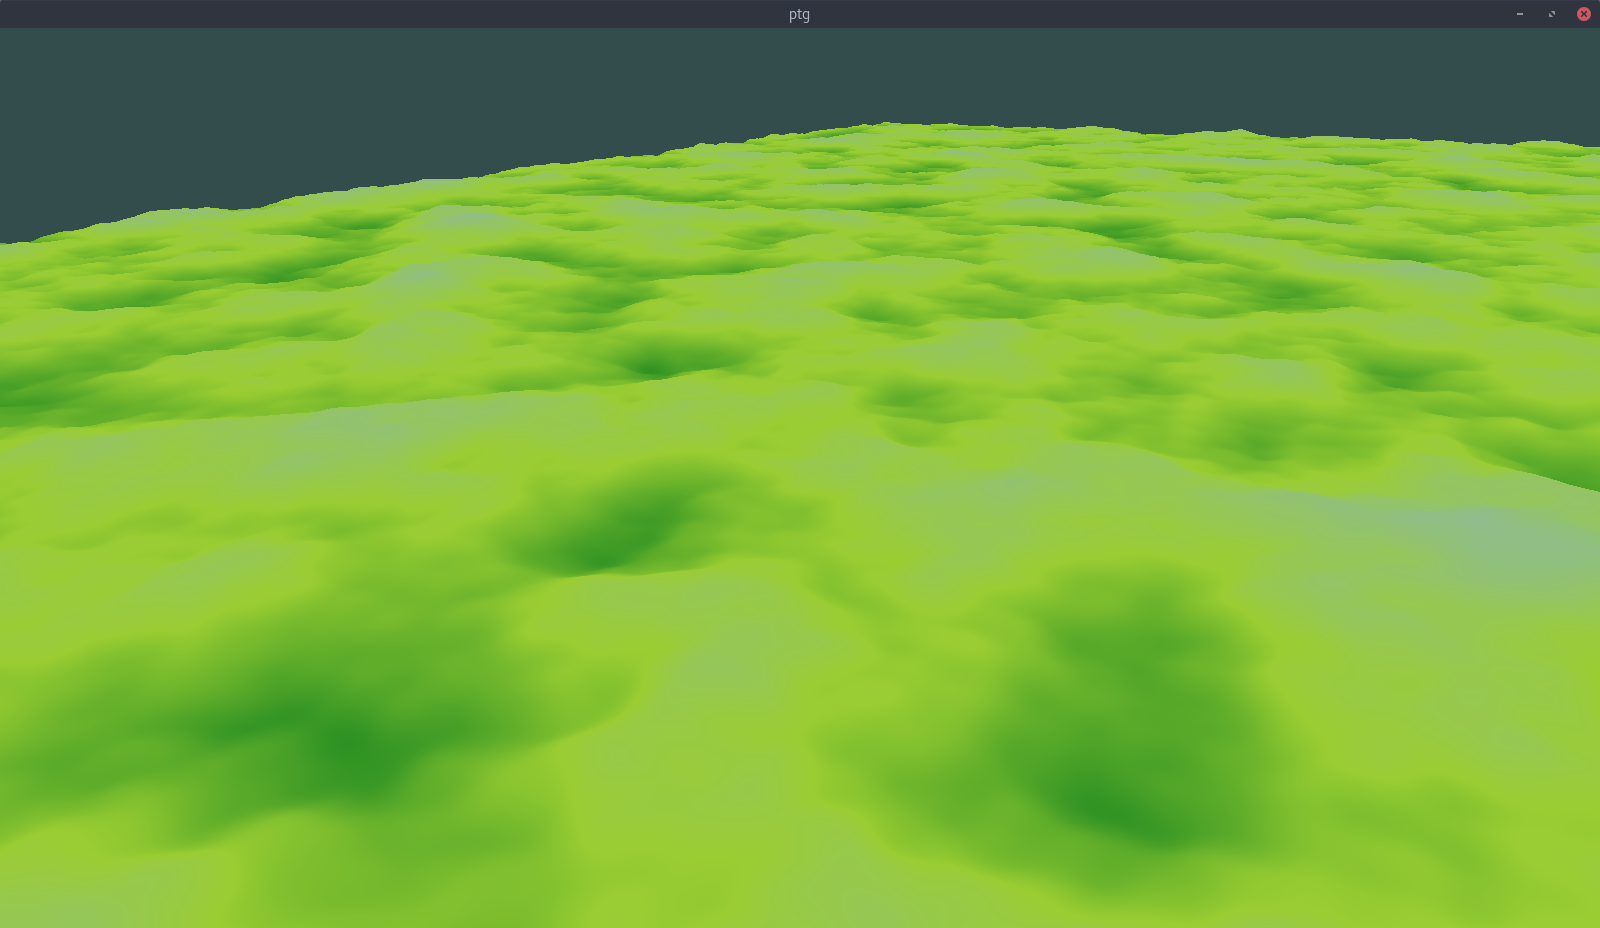
\includegraphics[width=0.48\textwidth]{figuras/bssPlains.png}\label{fig:biomaTipo1}}\hspace{0.1cm}
     \subfloat[][$biomaTipo =$ Montanhas]{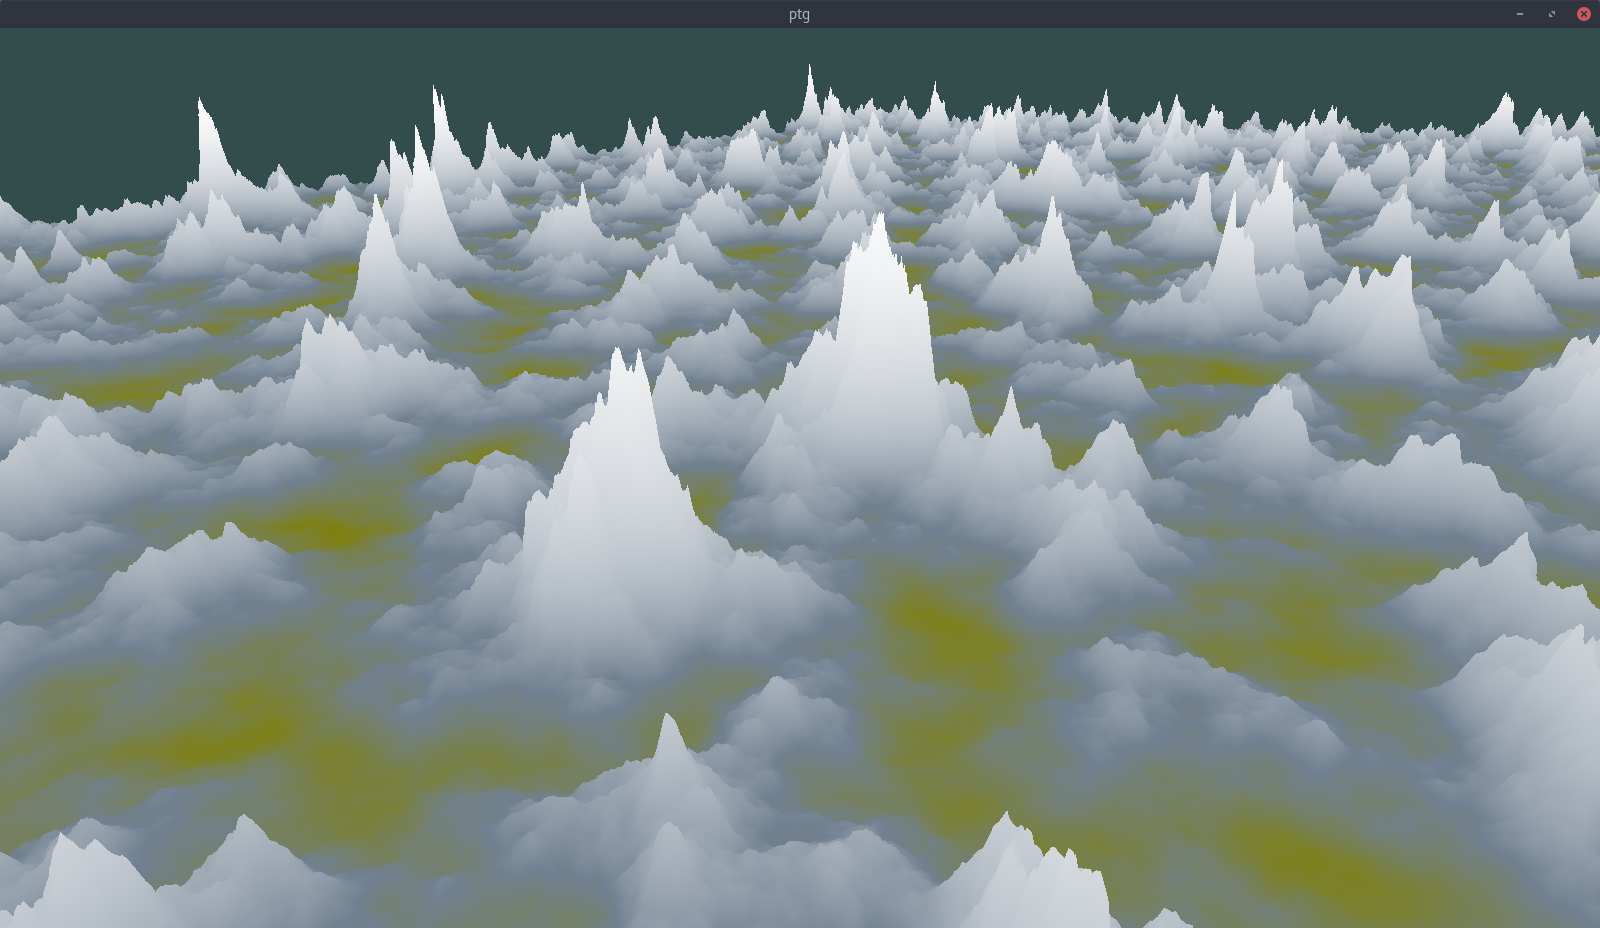
\includegraphics[width=0.48\textwidth]{figuras/bssMontains.png}\label{fig:biomaTipo2}}\\
     \subfloat[][$biomaTipo =$ Vales]{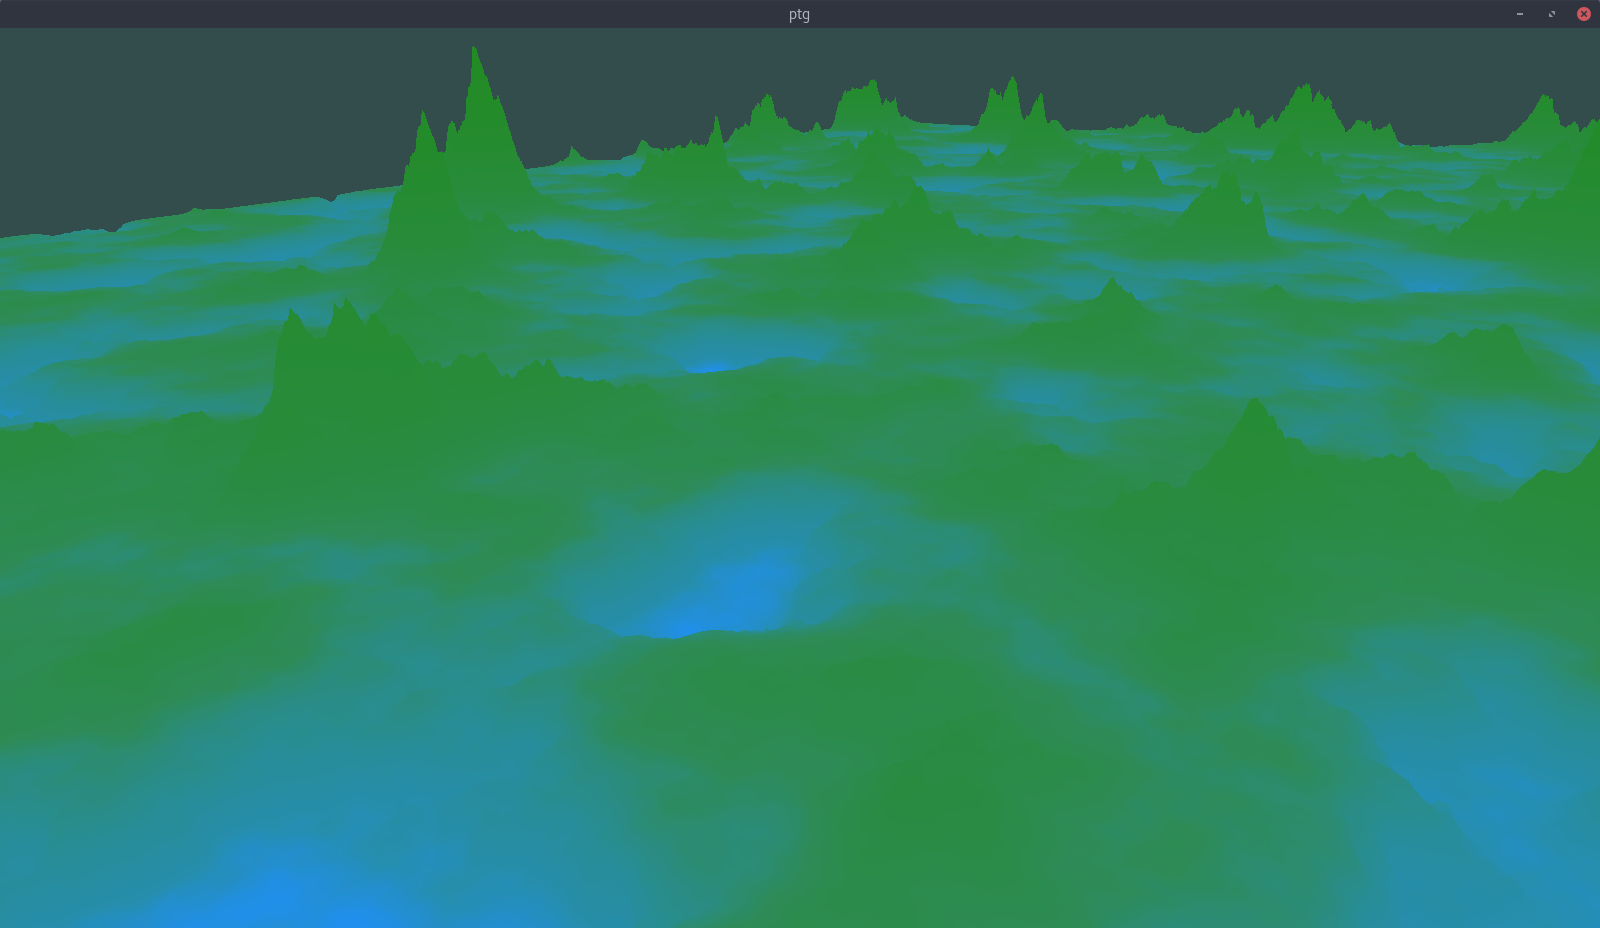
\includegraphics[width=0.48\textwidth]{figuras/bssValley.png}\label{fig:biomaTipo3}}\hspace{0.1cm}
     \subfloat[][$biomaTipo =$ Deserto]{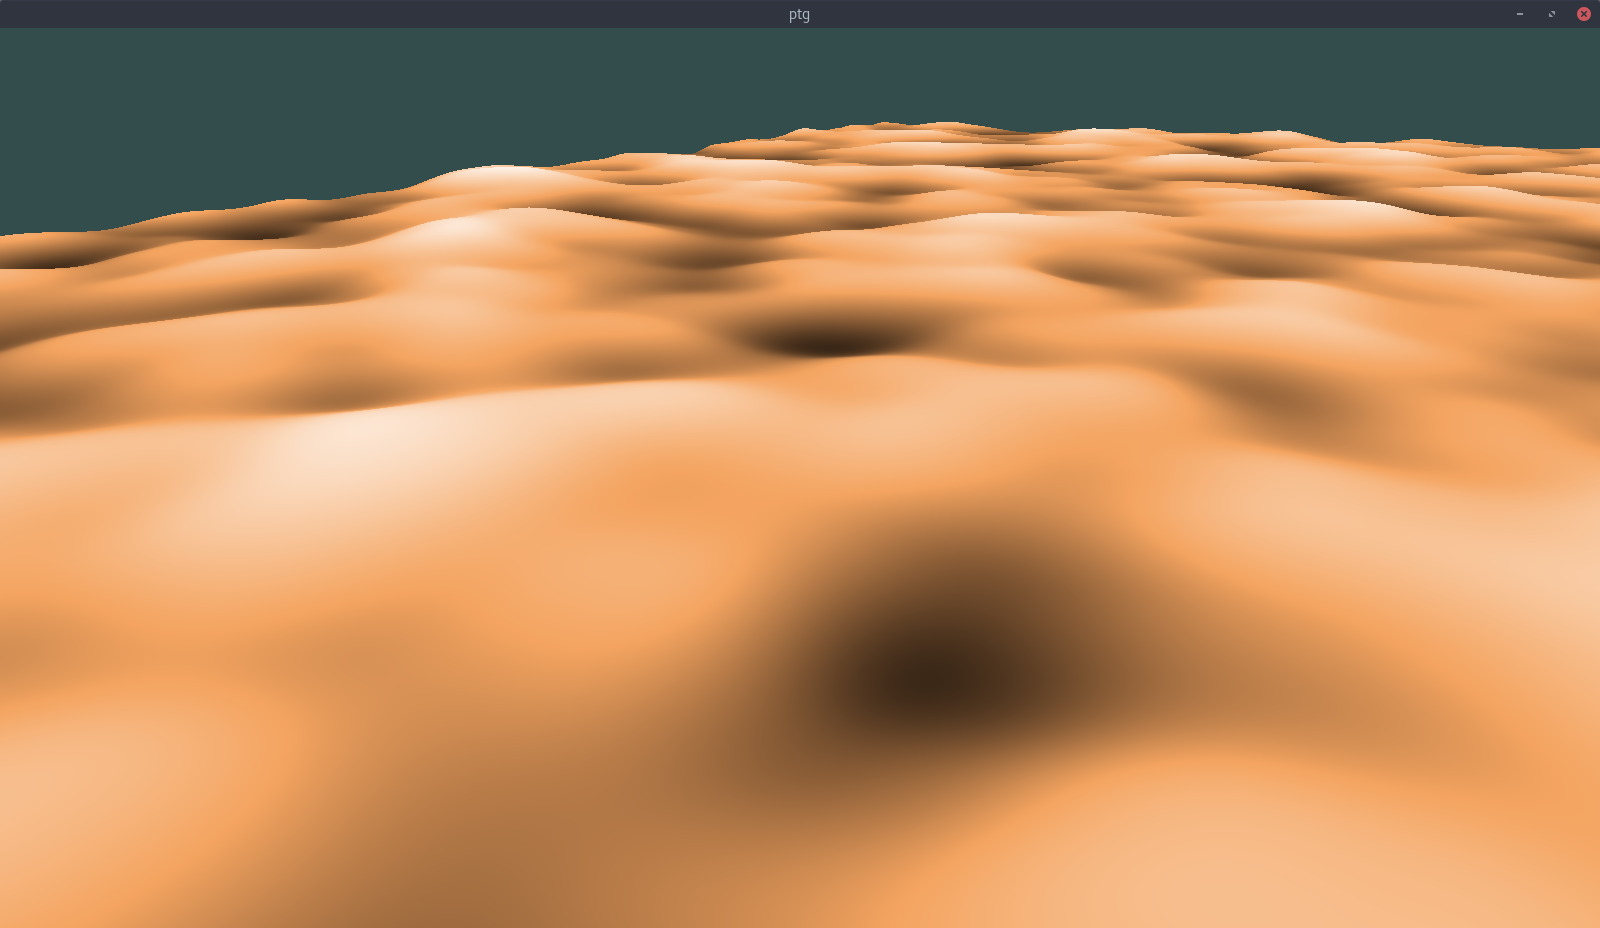
\includegraphics[width=0.48\textwidth]{figuras/bssDesert.png}\label{fig:biomaTipo4}}\\
     \subfloat[][$biomaTipo =$ Cânyons]{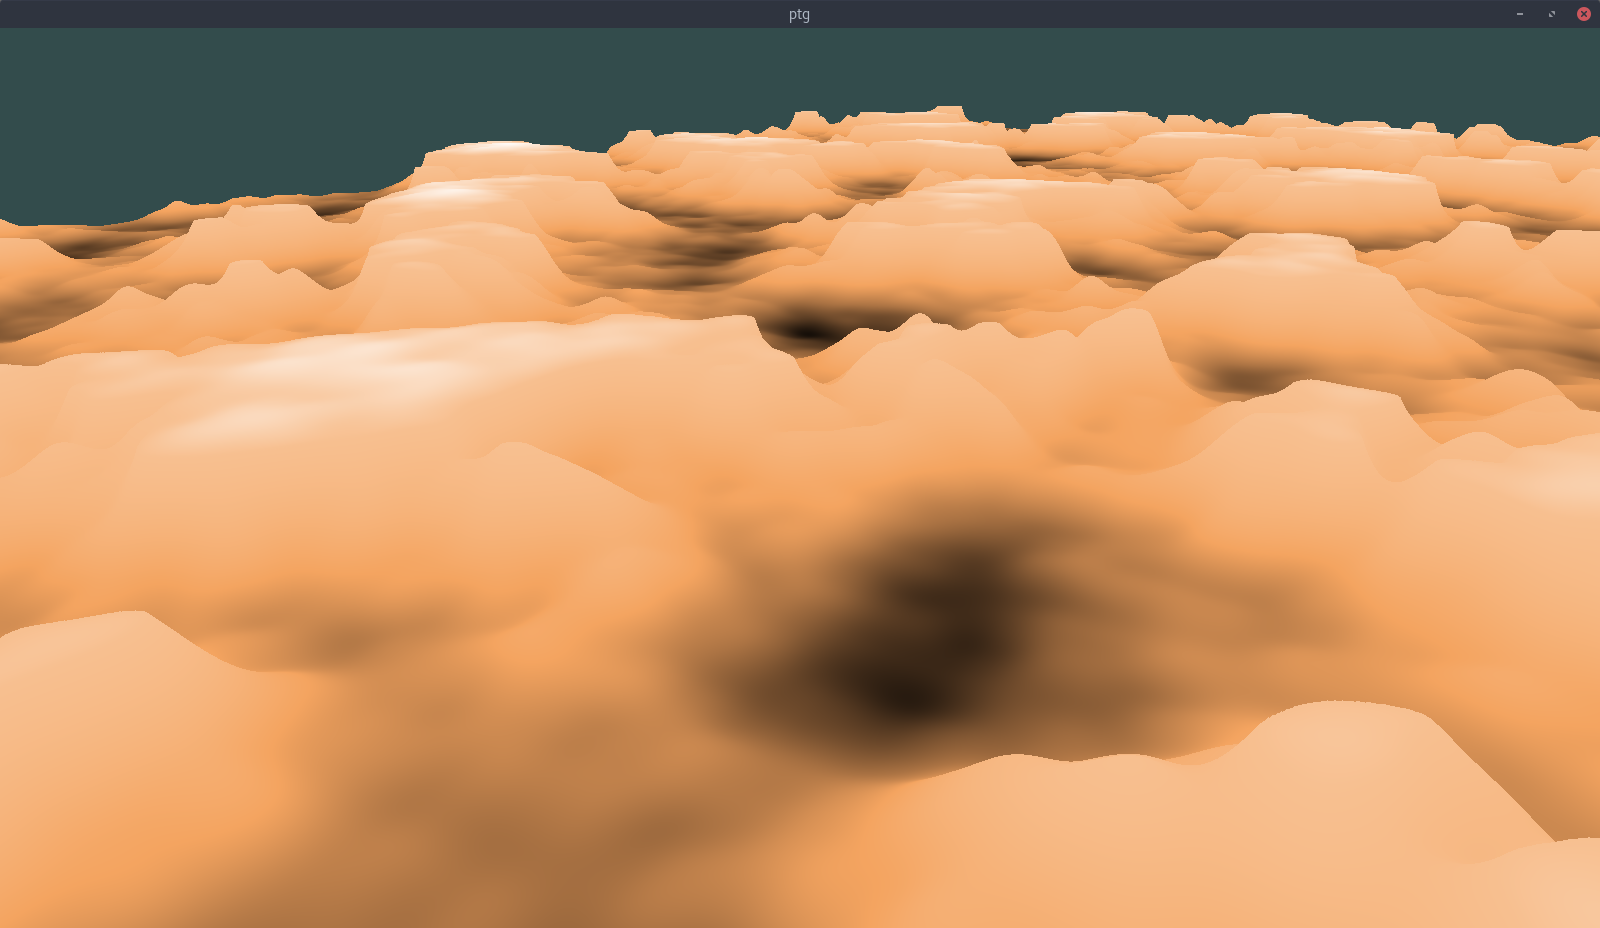
\includegraphics[width=0.48\textwidth]{figuras/bssCanyons.png}\label{fig:biomaTipo5}}
     
     \caption{Resultado dos Biomas fixados.}
     
     \label{fig:bssComBiomasFixados}
     % usar \hspace{0.1cm}, é gambiarra mas funciona
\end{figure}

\section{Separando Áreas de Biomas}
Para separar áreas de biomas com tamanho $b$ e escolher um $biomaTipo$ nessas áreas
vamos usar o seguinte algoritmo, considerando $dxs, dzs \in \mathbb{Q}$ e $di, dj \in \mathbb{N}$.

%DEBUG: explicar função trunc em algum lugar
\begin{algorithm}[H]\label{alg:getBiomeXZXadrez}
    $dxs \leftarrow x/b$\;
    $dzs \leftarrow z/b$\;
    \If {$dxs < 0$}{
        $dxs \leftarrow dxs - 1$\;
    }
    \If {$dzs < 0$}{
        $dzs \leftarrow dzs - 1$\;
    }
    $dxs \leftarrow$ trunc($dxs$)\;
    $dzs \leftarrow$ trunc($dzs$)\;
    $di \leftarrow dxs$\;
    $dj \leftarrow dzs$\;
    \If {$di$ é divisivel por $2$}{
        \If {$dj$ é divisivel por $2$}{
            $biomaTipo \leftarrow$ Montanhas\;
        }\Else{
            $biomaTipo \leftarrow$ Cânyons\;
        }
    }\Else{
        \If {$dj$ é divisivel por $2$}{
            $biomaTipo \leftarrow$ Cânyons\;
        }\Else{
            $biomaTipo \leftarrow$ Montanhas\;
        }
    }
    
    
    \caption{Escolhendo biomas em áreas de tamanho $b$, com áspecto xadrez.}
\end{algorithm}

Se remover as linhas 3 até 8 do algorimo \ref{alg:getBiomeXZXadrez} vamos ter o 
problema do valor $0$ se repetir em $di$ ou $dj$ nos valores de $0 < x, z < b$ e $0 > x, z > -b$, 
quando isso acontece temos os valores de $(di, dj)$ mostrados na
matriz $B_{b}$ gerando as áreas mostradas na figura \ref{fig:xadrez}. Mas quando essas
linhas do algoritmo estão inclusas os resultados estão representados na matriz $B_{a}$
e na figura \ref{fig:xadrez}. Os parâmetros para gerar as
imagens \ref{fig:ssxadrez} são: $\Delta_{v} = 0.5$, 
$k = 2048$, $ x_{s} = -k/2 , z_{s} = -k/2$, $b = 200$ e $seed = 3$.

\[
B_{a} = 
\begin{bmatrix}
    \ddots                & \vdots & \vdots & \vdots & \vdots & \vdots & \reflectbox{$\ddots$} \\
    \dots                 &(-2, 2) &(-1, 2) &(0, 2)  &(1, 2)  &(2, 2)  & \dots                 \\
    \dots                 &(-2, 1) &(-1, 1) &(0, 1)  &(1, 1)  &(2, 1)  & \dots                 \\
    \dots                 &(-2, 0) &(-1, 0) &(0, 0)  &(1, 0)  &(2, 0)  & \dots                 \\
    \dots                 &(-2, -1)&(-1, -1)&(0, -1) &(1, -1) &(2, -1) & \dots                 \\
    \dots                 &(-2, -2)&(-1, -2)&(0, -2) &(1, -2) &(2, -2) & \dots                 \\
    \reflectbox{$\ddots$} & \vdots & \vdots & \vdots & \vdots & \vdots & \ddots                \\
    
\end{bmatrix}
\]
\[
B_{b} = 
\begin{bmatrix}
    \ddots                & \vdots & \vdots & \vdots & \vdots & \vdots & \reflectbox{$\ddots$} \\
    \dots                 &(-1, 2) &(0, 2)  &(0, 2)  &(1, 2)  &(2, 2)  & \dots                 \\
    \dots                 &(-1, 1) &(0, 1)  &(0, 1)  &(1, 1)  &(2, 1)  & \dots                 \\
    \dots                 &(-1, 0) &(0, 0)  &(0, 0)  &(1, 0)  &(2, 0)  & \dots                 \\
    \dots                 &(-1, 0) &(0, 0)  &(0, 0)  &(1, 0)  &(2, 0) & \dots                 \\
    \dots                 &(-1, -1)&(0, -1) &(0, -1) &(1, -1) &(2, -1) & \dots                 \\
    \reflectbox{$\ddots$} & \vdots & \vdots & \vdots & \vdots & \vdots & \ddots                \\
    
\end{bmatrix}
\]

 
\begin{figure}[H]
     \centering
     \subfloat[][sem usar linhas 3 à 8]{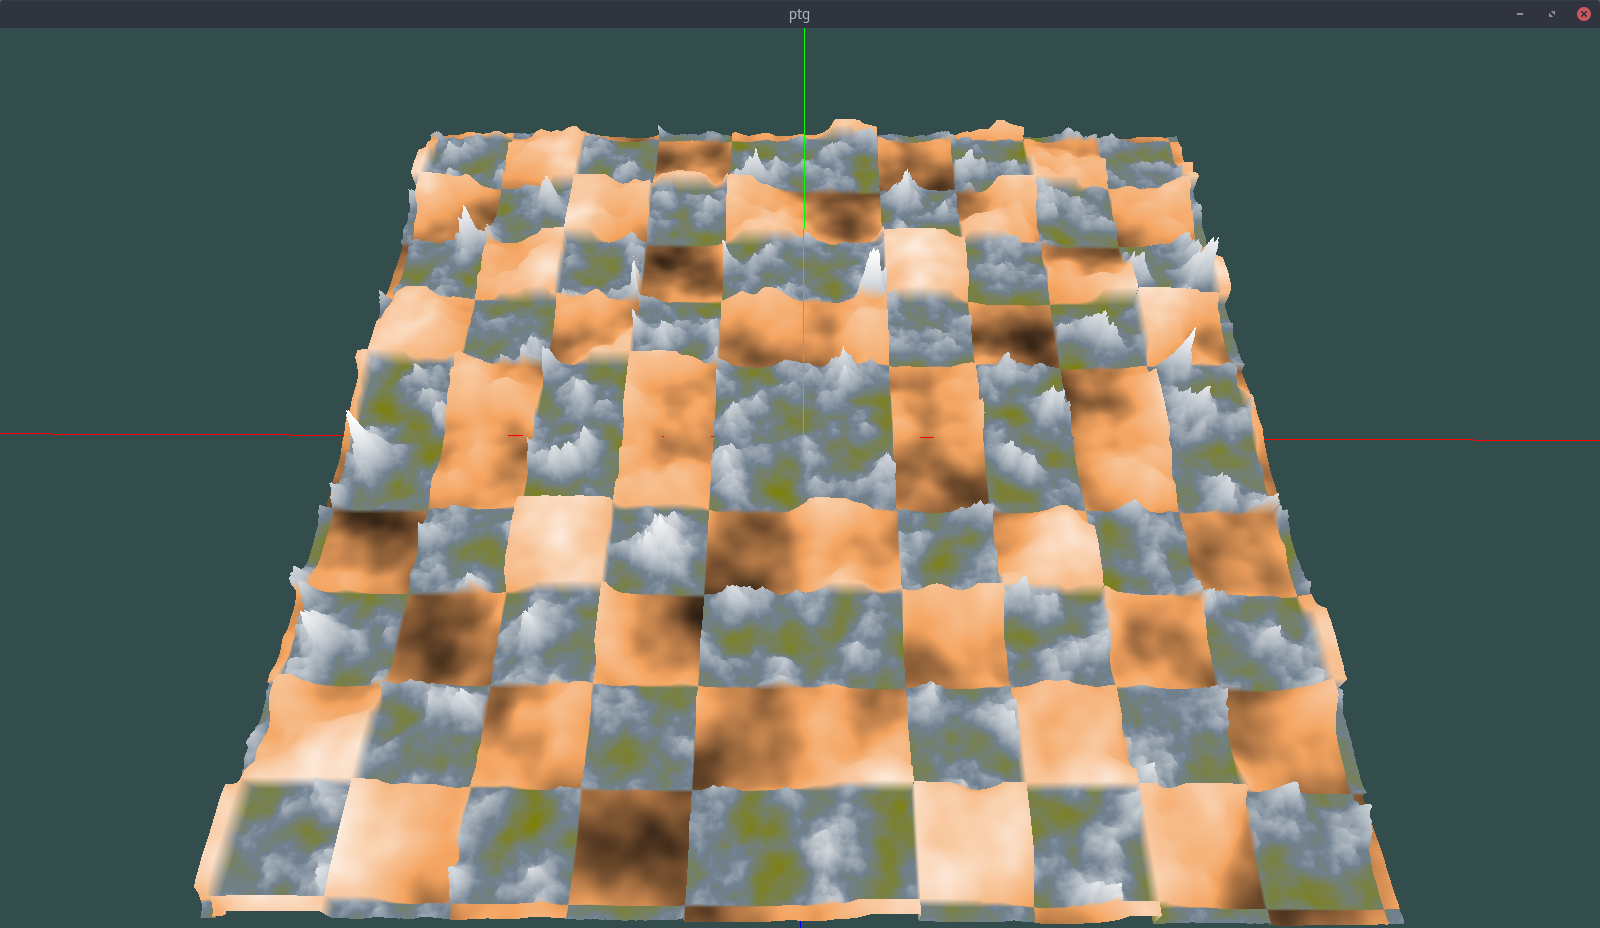
\includegraphics[width=0.48\textwidth]{figuras/didjissue.png}\label{fig:xadrez}}\hspace{0.1cm}
     \subfloat[][Usando as linhas 3 à 8]{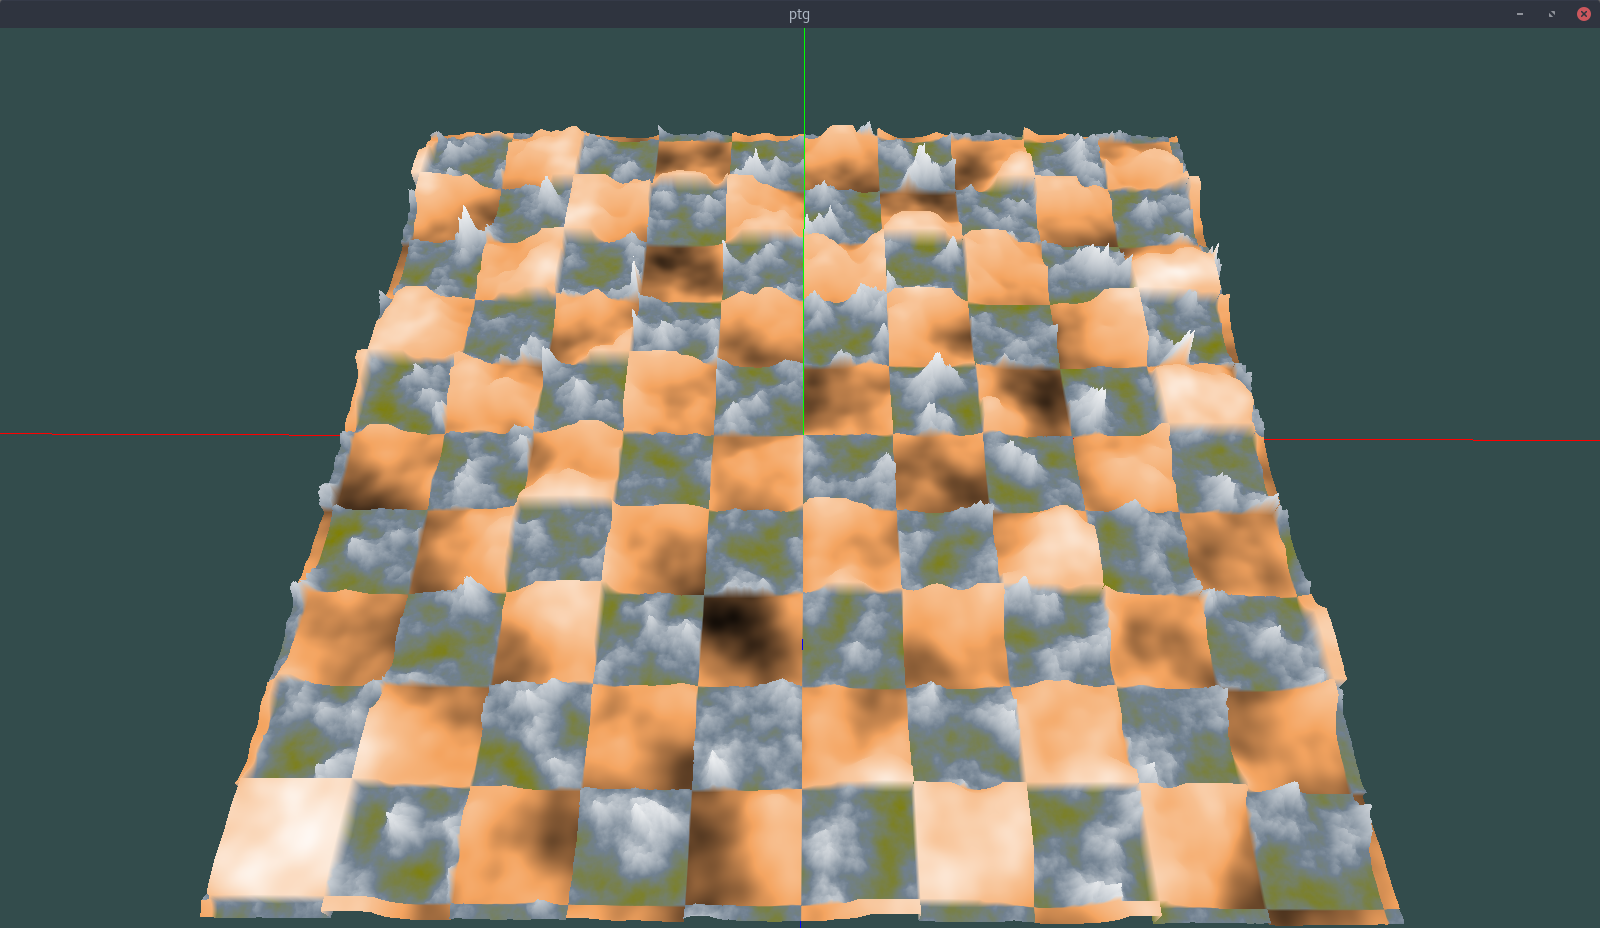
\includegraphics[width=0.48\textwidth]{figuras/didjissuefix.png}\label{fig:xadrezFix}}\\
     
     \caption{Mostrando a influência das linhas 3 até 8 no algoritmo \ref{alg:getBiomeXZXadrez}.}
     
     \label{fig:ssxadrez}
     % usar \hspace{0.1cm}, é gambiarra mas funciona
\end{figure}

Mas a intenção não é criar divisões nesse estilo de "xadrez" então será usado um 
ruído como parametros $dxs$ e $dzs$ para definir o bioma de cada região é usado
o algoritmo \ref{alg:getBiomeXZ}.

\begin{algorithm}[H]\label{alg:getBiomeXZ}
    \SetKwInOut{Input}{entrada}\SetKwInOut{Output}{output}
    \Input{$x \in \mathbb{Q}, z \in \mathbb{Q}$}
    $dxs \leftarrow x/b$\;
    $dzs \leftarrow z/b$\;
    \If {$dxs < 0$}{
        $dxs \leftarrow dxs - 1$\;
    }
    \If {$dzs < 0$}{
        $dzs \leftarrow dzs - 1$\;
    }
    $dxs \leftarrow$ trunc($dxs$)\;
    $dzs \leftarrow$ trunc($dzs$)\;
    
    $areaValue \leftarrow$ Noise$((dxs + const)/fb, (dzs + const)/fb)$\;
    $areaValue \leftarrow  areaValue \cdot 0.5 + 0.5$\;
    $areaValue \leftarrow$ clamp($areaValue, 0, 0.99$)\;
    $biomaTipo \leftarrow$ trunc($areaValue \cdot \bar{N}$)\;\tcc{$\bar{N} = 5$ Quantidade de biomas distintos}
    retorna $biomaTipo$\;
    \caption{Escolhendo biomas em áreas de tamanho $b$.}
\end{algorithm}

A variável $biomaTipo$ tem valoração inteira, então é possivel olhar a tabela \ref{tab:bioColors}
o campo int id para saber qual valor inteiro é associado a qual bioma, $biomaTipo \in \{$Planícies, Montanhas, Vales, Deserto, Cânyons$\}$
$fb$ é a variavel que dita a frequencia na variação de biomas e $const$ é uma constante,
$const \in \mathbb{Q}$, a constante previne que o parametro seja sempre inteiro, quando $fb$ é um valor muito baixo,
a possibilidade de dxs e dzs serem inteiros é grande e quando parâmetros de Noise 
são inteiros então seu retorno sempre será $0$ \cite{perlin1985image}. Todos os resultados 
neste trabalho usam $const = 7.3$ escolhido arbitrariamente.

Os parâmetros usados na figura \ref{fig:biomeareasanotherComp} são: $\Delta_{v} = 0.5$, 
$k = 2048$, $b = 200$ e $seed = 3$. em duas chunks a primeira com $ x_{s} = -k/2 , z_{s} = -k/2$
e a segunda com $ x_{s} = 1023 , z_{s} = -k/2$.

\begin{figure}[H]
     \centering
     \subfloat[][$fb = 0.5$]{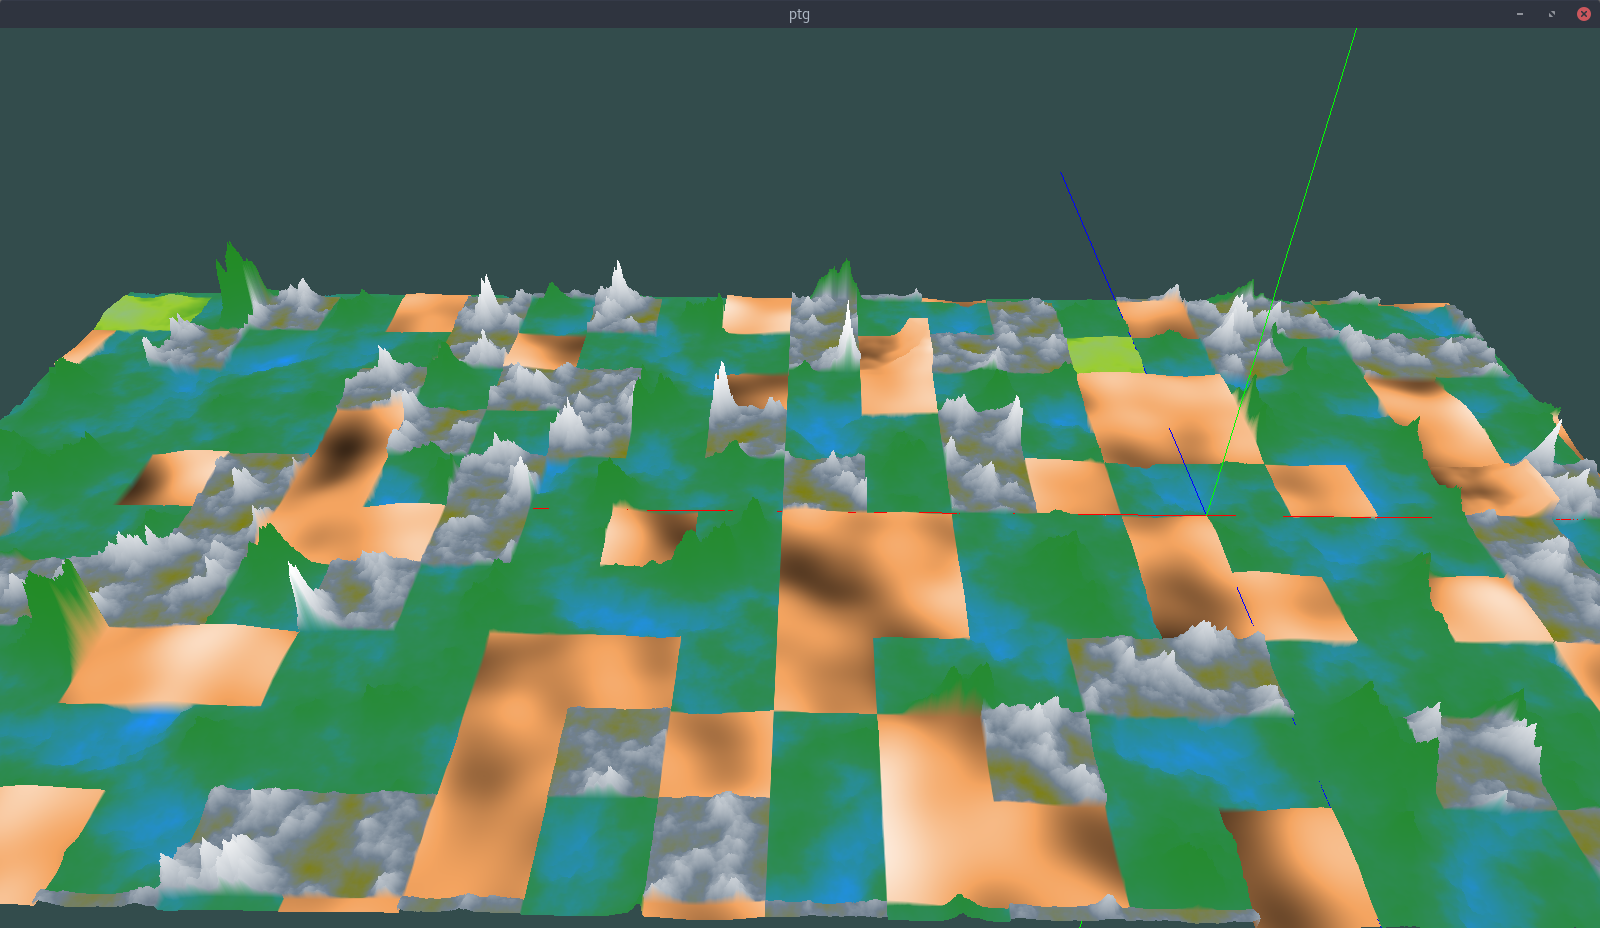
\includegraphics[width=0.48\textwidth]{figuras/fbl/fb05l200.png}\label{fig:fb05l200}}\hspace{0.1cm}
     \subfloat[][$fb = 4$]{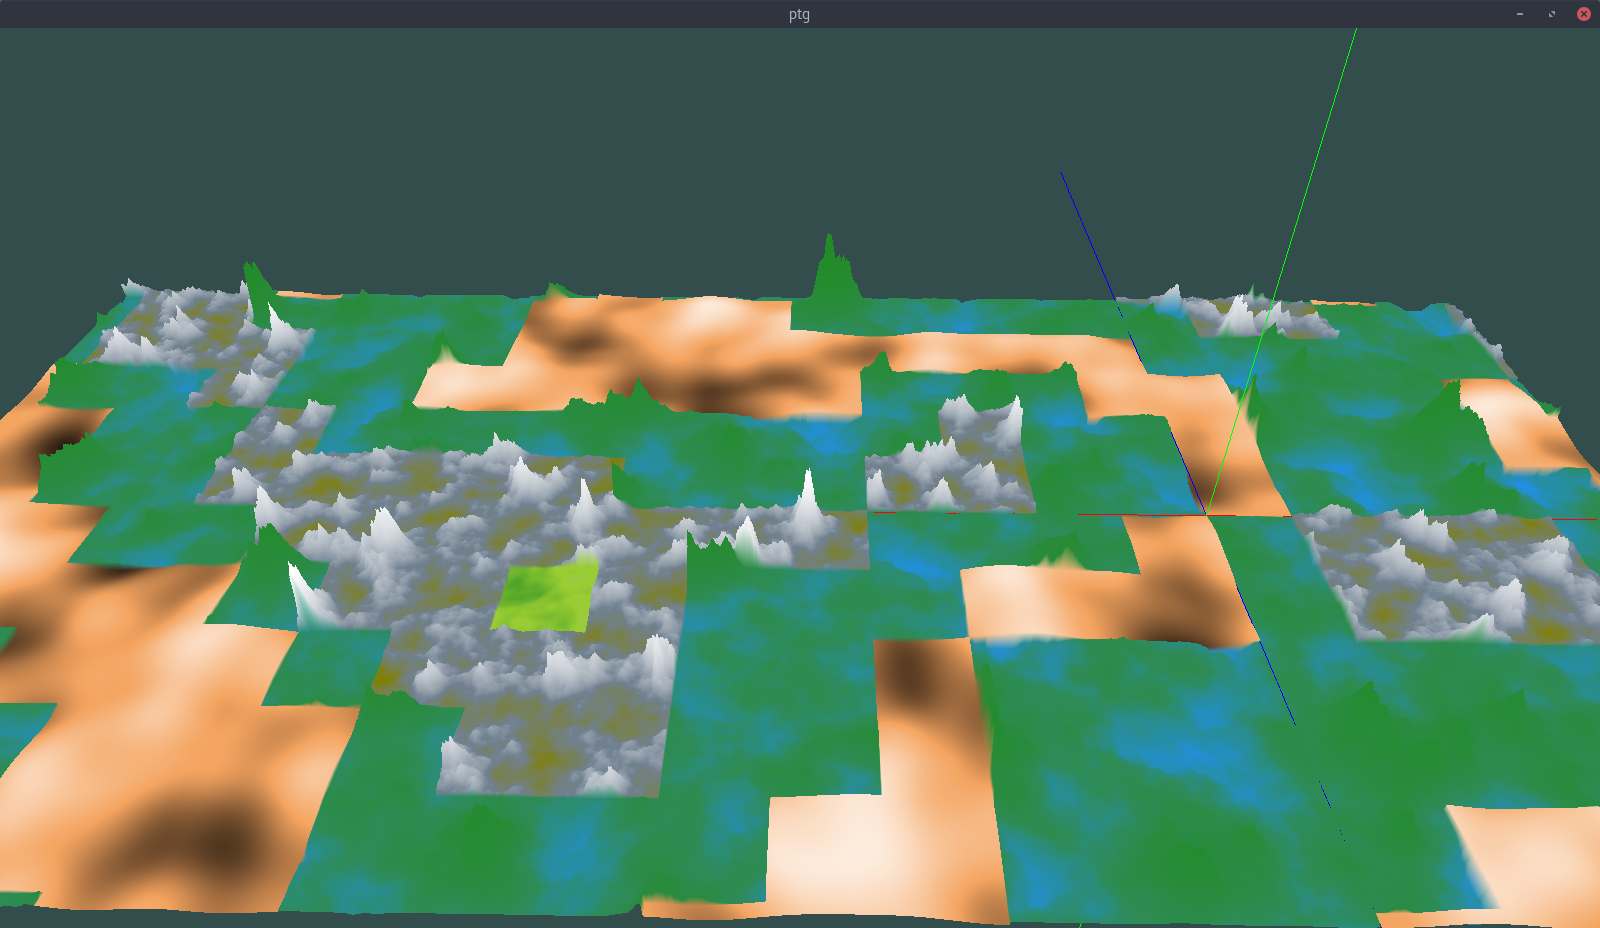
\includegraphics[width=0.48\textwidth]{figuras/fbl/fb4l200.png}\label{fig:fb4l200}}\\
     \subfloat[][$fb = 10$]{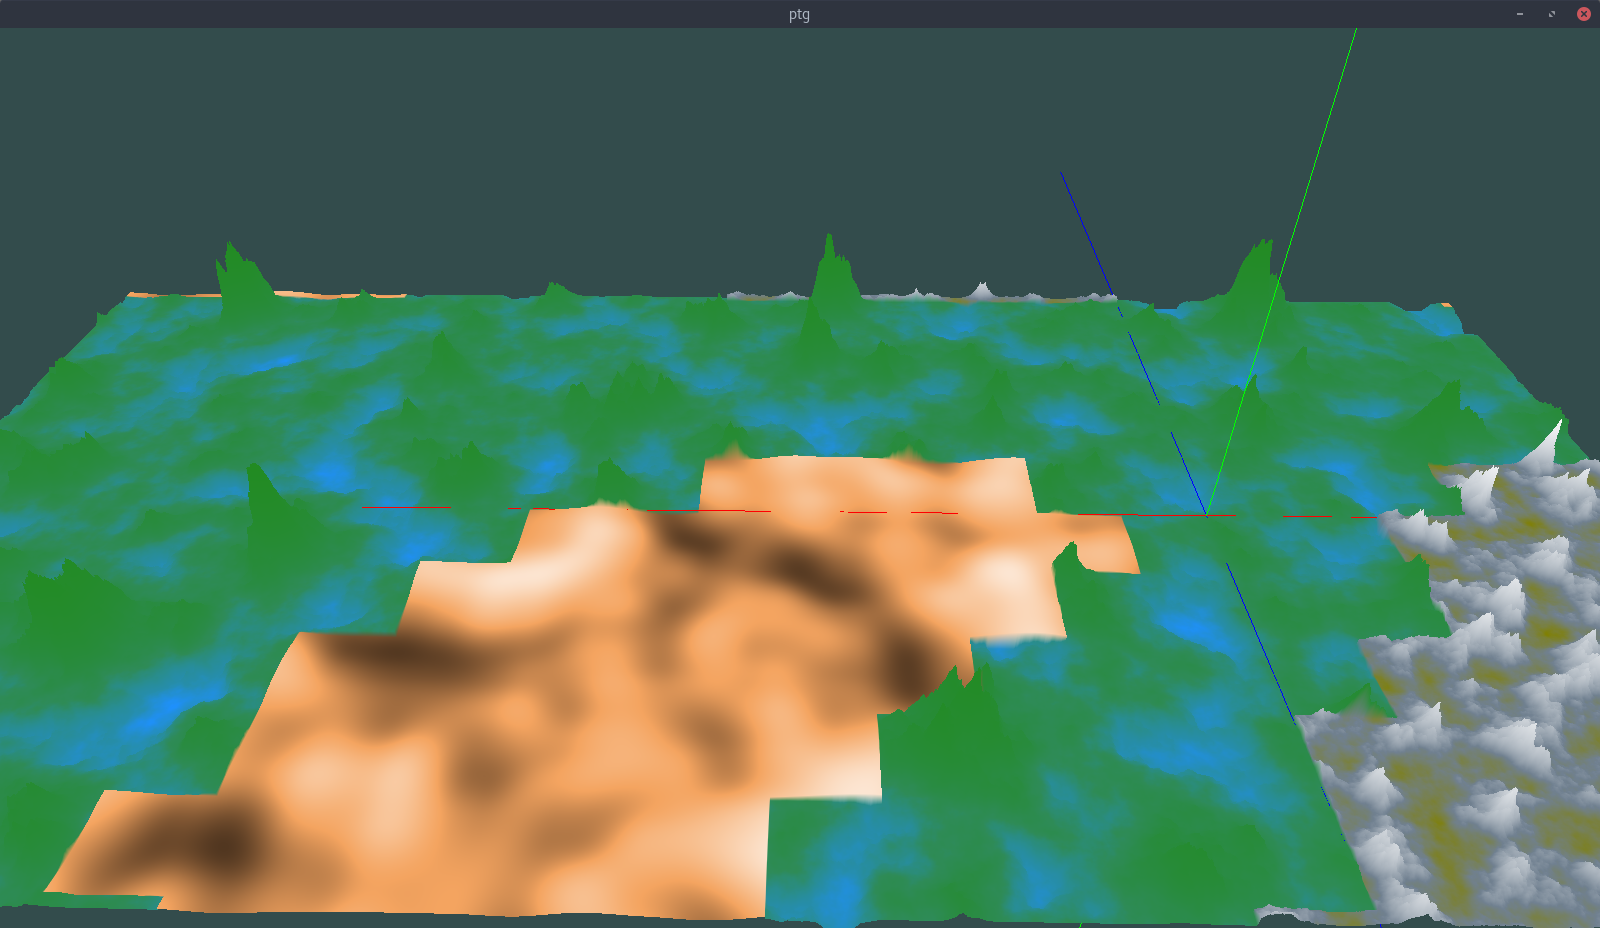
\includegraphics[width=0.48\textwidth]{figuras/fbl/fb10l200.png}\label{fig:fb10l200}}\hspace{0.1cm}
     \subfloat[][$fb = 25$]{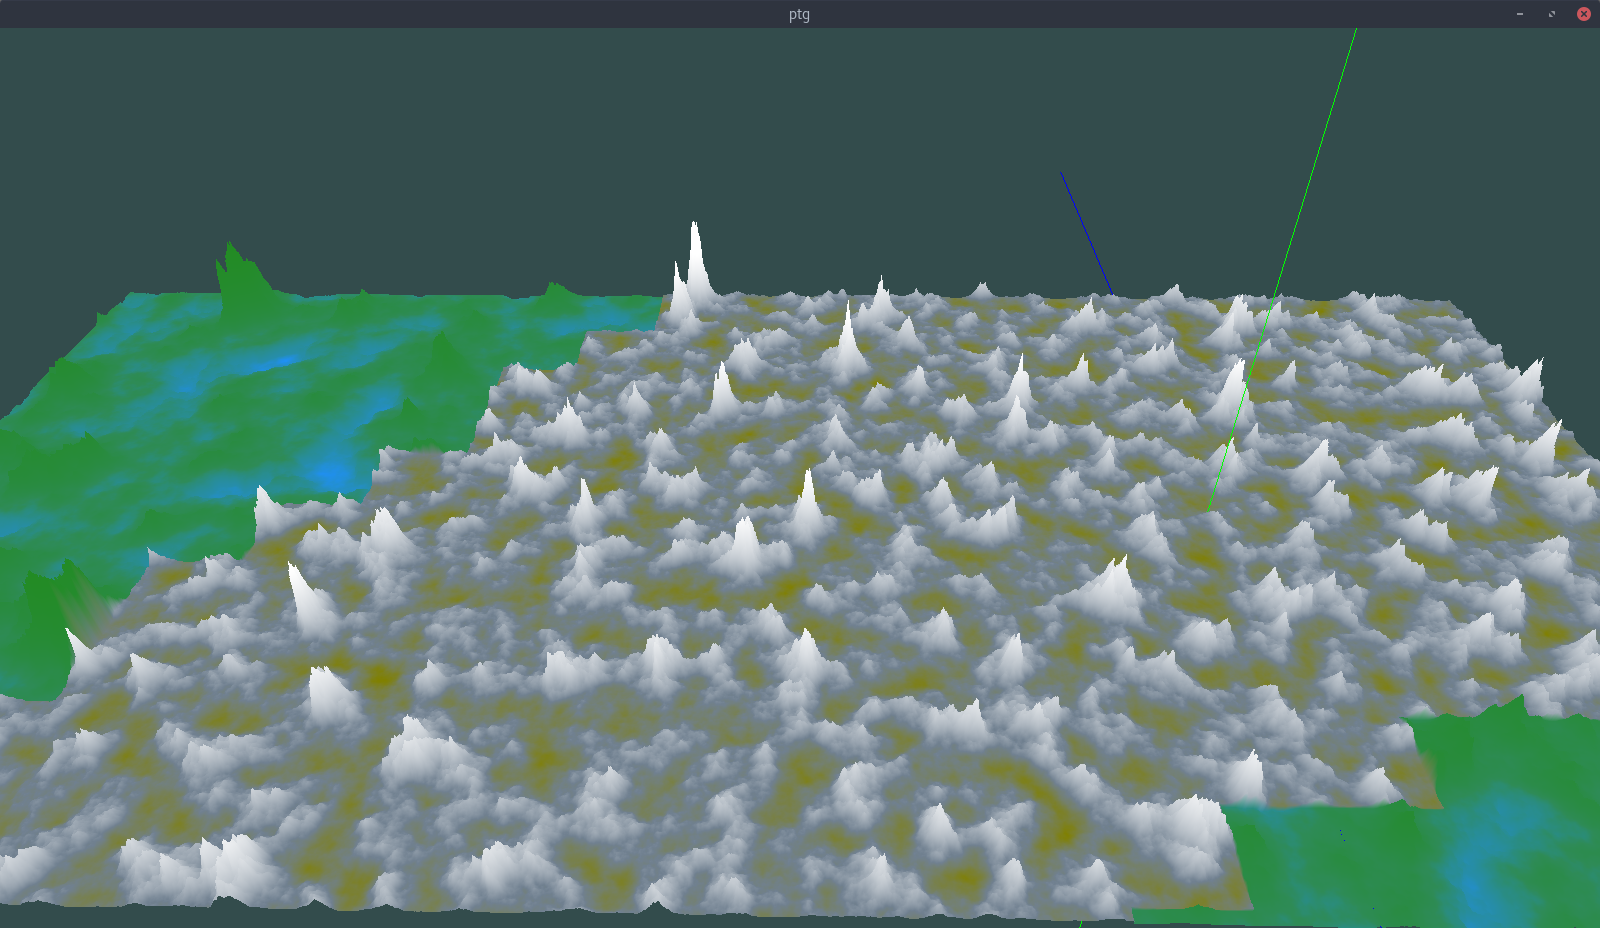
\includegraphics[width=0.48\textwidth]{figuras/fbl/fb25l200.png}\label{fig:fb25l200}}
     \caption{Diferença entre frequencia de biomas.}
     
     \label{fig:biomeareasanotherComp}
     % usar \hspace{0.1cm}, é gambiarra mas funciona
\end{figure}

A figura \ref{fig:biomeareasanotherCompx} quase usa os mesmos parâmetros que imagens \ref{fig:biomeareasanotherComp}
com diferença que desta vez $b = 512$.

\begin{figure}[H]
     \centering
     \subfloat[][$fb = 0.5$]{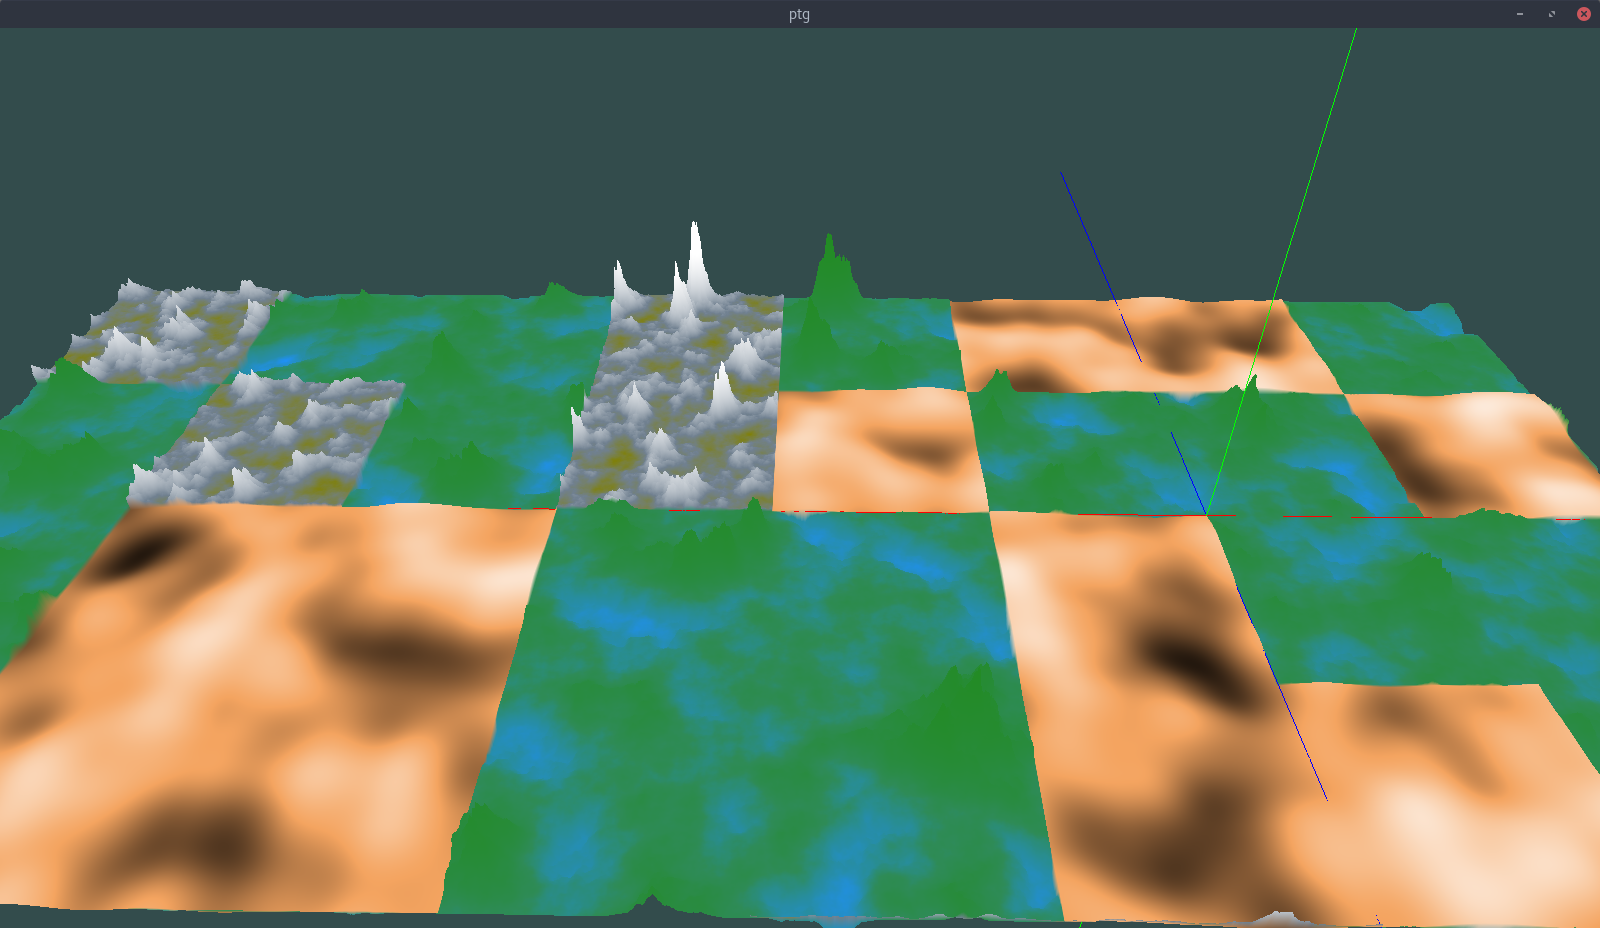
\includegraphics[width=0.48\textwidth]{figuras/fbl/fb05l512.png}\label{fig:fb05l512}}\hspace{0.1cm}
     \subfloat[][$fb = 50$]{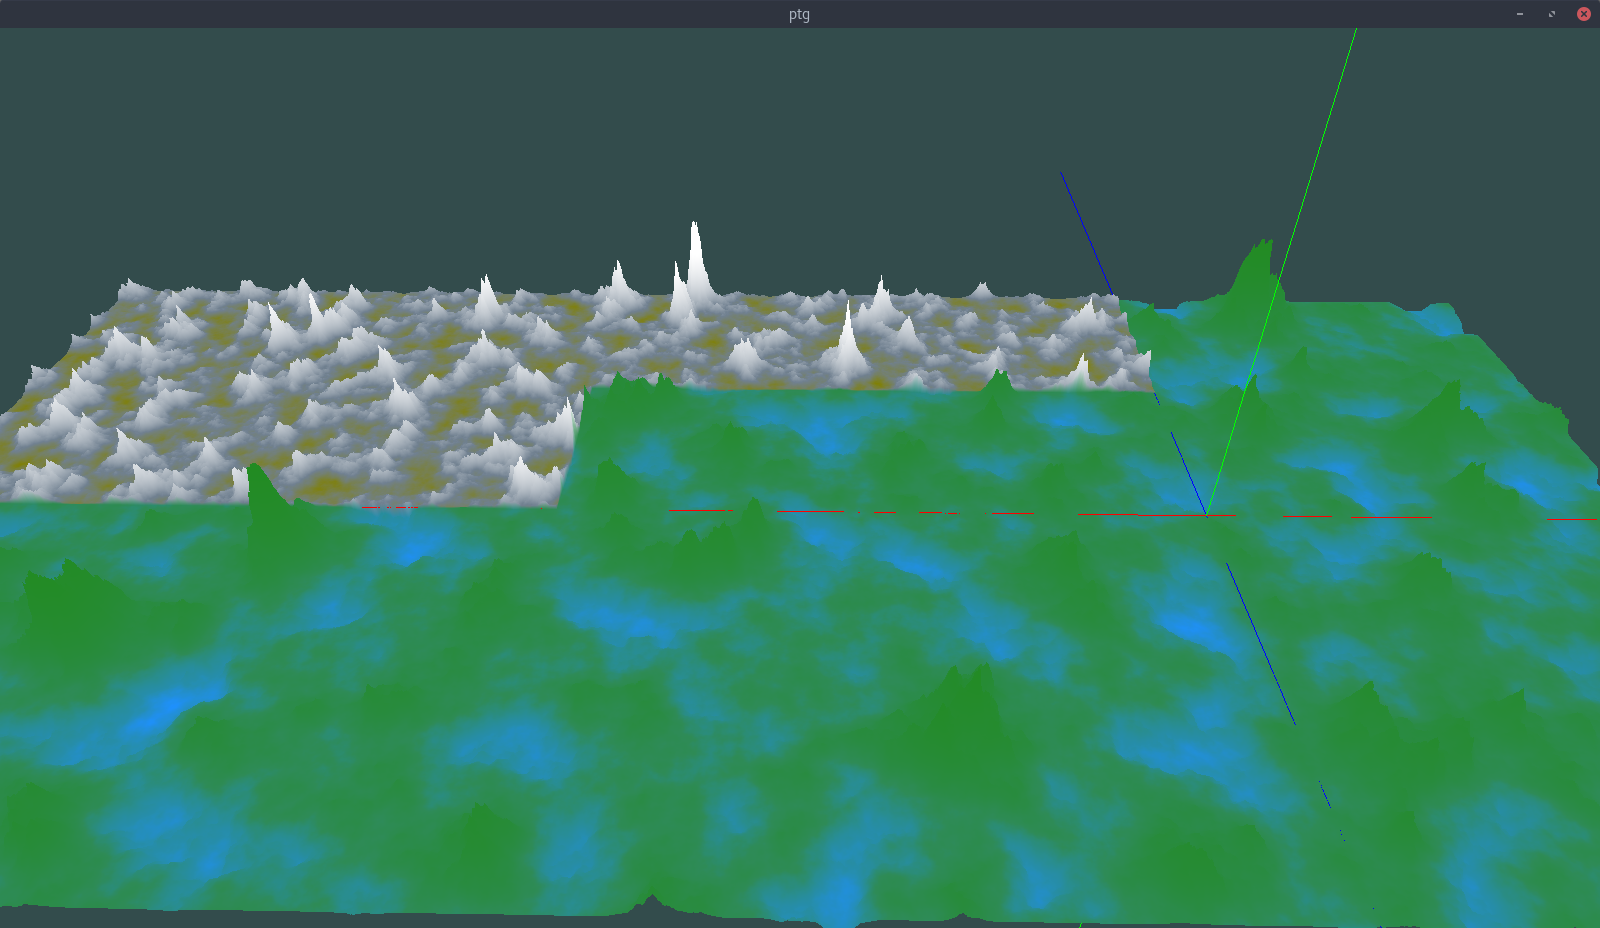
\includegraphics[width=0.48\textwidth]{figuras/fbl/fb50l512.png}\label{fig:fb50l512}}\\
     \caption{Diferença entre frequencia de biomas com $b = 512$.}
     
     \label{fig:biomeareasanotherCompx}
     % usar \hspace{0.1cm}, é gambiarra mas funciona
\end{figure}

\section{Detectando fronteira entre Biomas}

Porem da maneira que está as fronteiras entre os biomas não tem um terreno
contínuo, como é visivel na imagem \ref{fig:descontinuos}, em uma aplicação para jogos
dificultaria consideravelmente
a jogabilidade neste terreno. %descontinuos.png

\begin{figure}[H]
    \centering
    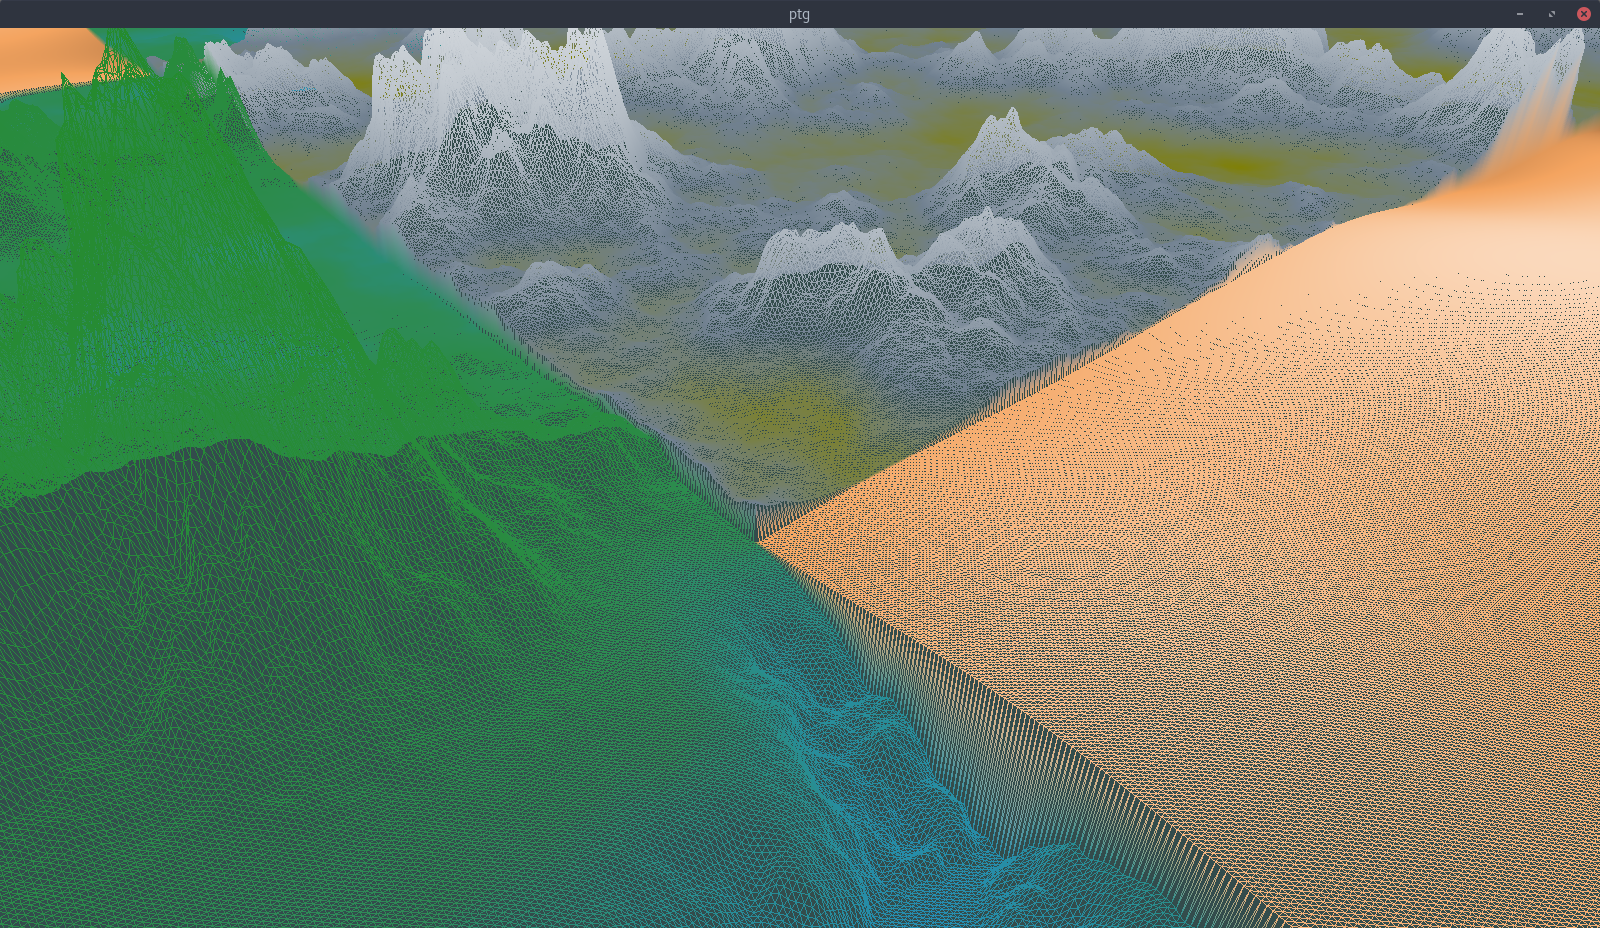
\includegraphics[width=0.75\textwidth]{figuras/descontinuos.png}
    \caption{Terreno com fronteira descontinua.}
    \label{fig:descontinuos}
\end{figure}

Para detectar a proximidade de um vértice a alguma fronteira podemos calcular o 
quão próximo ele está de algum ponto dívisivel por $b$, isso será feito com 
o algoritmo \ref{alg:borderTest}. O algoritmo recebe uma entrada $in$ e calcula
a distância euclidiana unidimensional com o valor divisivel por $b$ mais próximo 
de $in$. Caso essa distância for menor que $l$ então o vértice em questão é 
fronteira.

O algoritmo \ref{alg:borderTest} retorna uma estrutra $BH$, com as informações
se o parâmetro é uma fronteira $BH.bordaFlag \in \{true, false\}$, se a fronteira 
está acima da entrada $BH.acimaFlag \in \{true, false\}$ e a distância relativa 
da fronteira $BH.pDist \in \mathbb{Q}: 0 \leq BH.pDist \leq 1$, caso a distância de $in$ até $b$ for bem 
próxima de $l$ e menor que $l$ então o valor de $BH.pDist$ será proporcionalmente
próximo a $1$. As variáveis
$in^{\star}, borda', borada'' \in \mathbb{N}$ e $BH.pDist \in \mathbb{Q}$.

\begin{algorithm}[H]\label{alg:borderTest}%Usando parâmetro e não k
    \SetKwInOut{Input}{entrada}\SetKwInOut{Output}{output}
    \Input{$in \in \mathbb{Q}$}
    $negativeFlag \leftarrow in < 0$ ? true : false\;
    \tcc{$in^{\star} \in \mathbb{N}$, então $in^{\star}$ vai receber um valor truncado}
    $in^{\star} \leftarrow negativeFlag$ ? $-in$ : $in$\;
    \tcc{($in^{\star}/b$) divisão entre dois inteiros será outro inteiro}
    $borda' \leftarrow (in^{\star}/b +1) \cdot b$\;
    $borda'' \leftarrow (in^{\star}/b) \cdot b$\;
    
    \If {$negativeFlag$}{
        $borda' \leftarrow -borada'$\;
        $borada'' \leftarrow -borada''$\;
    }
    \tcc{Precisamos respeitar a restrição $l < b/2$ para o algoritmo entrar em apenas um dos seguintes casos}
    \If {abs$(borda' - in) < l$}{
        \tcc{Caso1: $in$ é fronteira, e a fronteira está acima de $in$}
        $BH.bordaFlag \leftarrow $true\;
        $BH.acimaFlag \leftarrow $true\;
        $BH.pDist \leftarrow$ abs$(borda' - in)/ l$\;
    }
    \uElseIf{abs$(borda'' - in) < l$}{
        \tcc{Caso2: $in$ é fronteira, e a fronteira está abaixo de $in$}
        $BH.bordaFlag \leftarrow $true\;
        $BH.acimaFlag \leftarrow $false\;
        $BH.pDist \leftarrow$ abs$(borda'' - in)/ l$\;
    }
    \Else{
        \tcc{Caso3: $in$ não é fronteira}
        $BH.bordaFlag \leftarrow $false\;
    }
    \If {$negativeFlag$}{
        $BH.acimaFlag \leftarrow \neg BH.acimaFlag$\;
    }
    retorna $BH$\;
    \caption{Teste de fronteira.}
\end{algorithm}

Para analisar esse valoers é possivel colorir as fronteiras...

\begin{algorithm}[H]\label{alg:borderColor}%Usando parâmetro e não k
    $BH_{x} \leftarrow$ Algoritmo\ref{alg:borderTest}($x$)\;
    $BH_{z} \leftarrow$ Algoritmo\ref{alg:borderTest}($z$)\;
    
    \If {$BH_{x}.bordaFlag$}{
        \If {$BH_{x}.acimaFlag$}{
            $cor \leftarrow$ mix($(0, 0, 0)$, $cor$, $peso$)\;\tcc{Preto}
        }\Else{
            $cor \leftarrow$ mix($(1, 1, 1)$, $cor$, $peso$)\;\tcc{Branco}
        }
    }
    \If {$BH_{z}.bordaFlag$}{
        \If {$BH_{z}.acimaFlag$}{
            $cor \leftarrow$ mix($(1, 0, 0)$, $cor$, $peso$)\;\tcc{Vermelho}
        }\Else{
            $cor \leftarrow$ mix($(0, 0, 1)$, $cor$, $peso$)\;\tcc{Azul}
        }
    }
    
    \caption{Colorindo fronteira.}
\end{algorithm}

Executando o algoritmo \ref{alg:borderColor} com $peso = 0.5$. $\Delta_{v} = 0.5$, 
$k = 2048$, $b = 512$, $seed = 3$ e $fb = 0.5$. em duas chunks a primeira com $ x_{s} = -k/2 , z_{s} = -k/2$
e a segunda com $ x_{s} = 1023 , z_{s} = -k/2$.

\begin{figure}[H]
     \centering
     \subfloat[][$l = 32$]{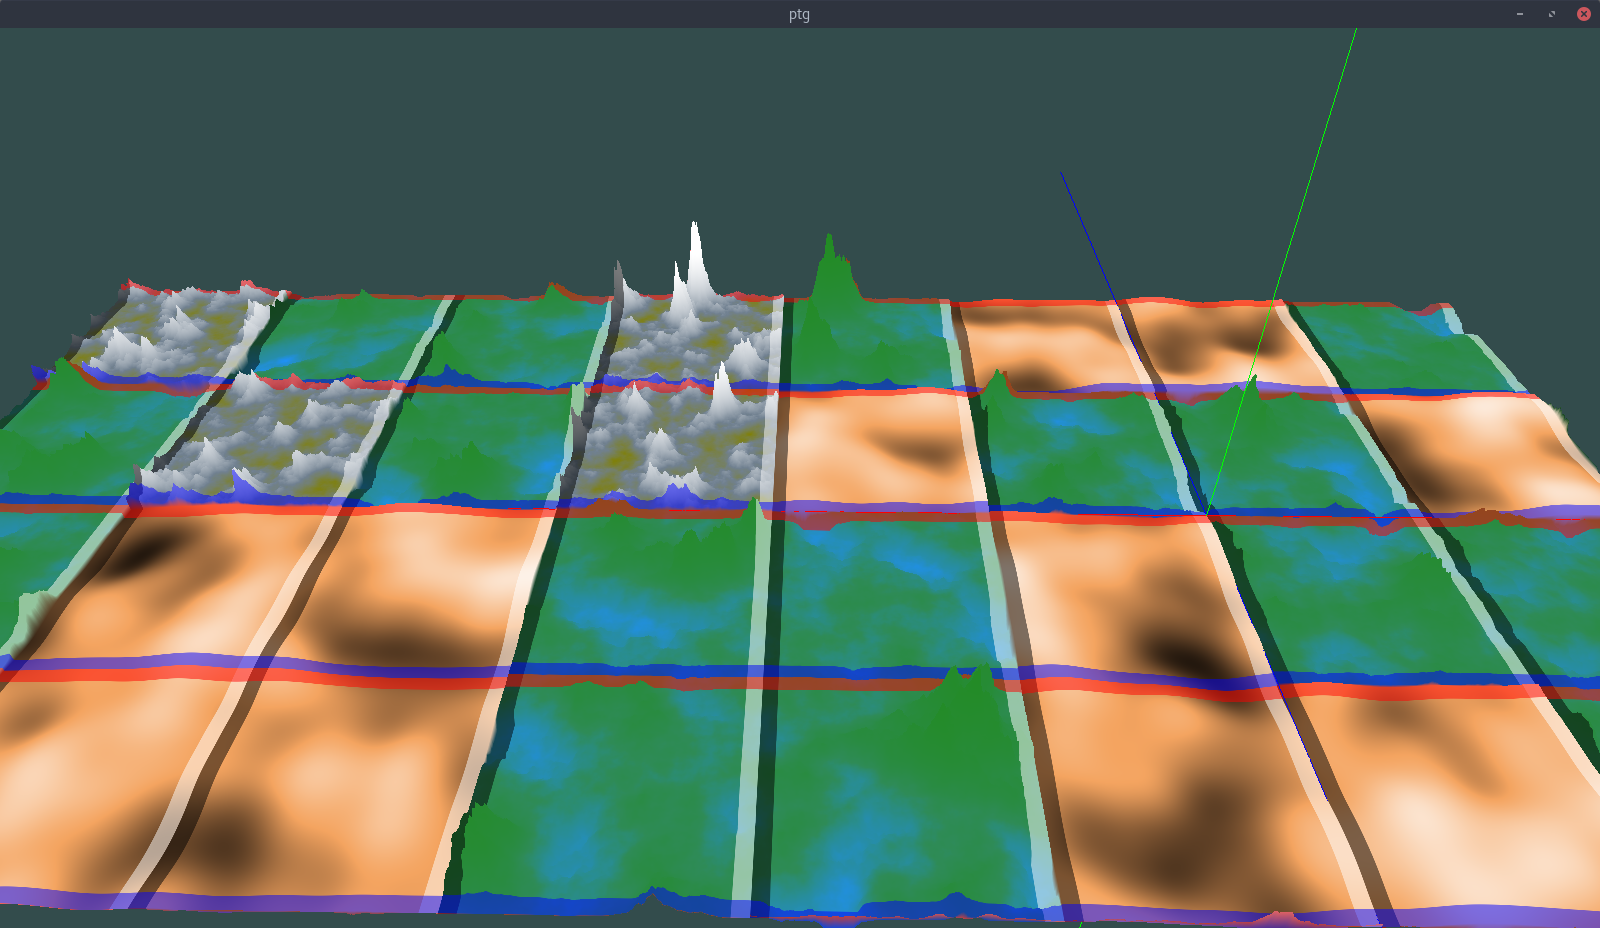
\includegraphics[width=0.48\textwidth]{figuras/border/l32.png}\label{fig:l32np}}\hspace{0.1cm}
     \subfloat[][$l = 128$]{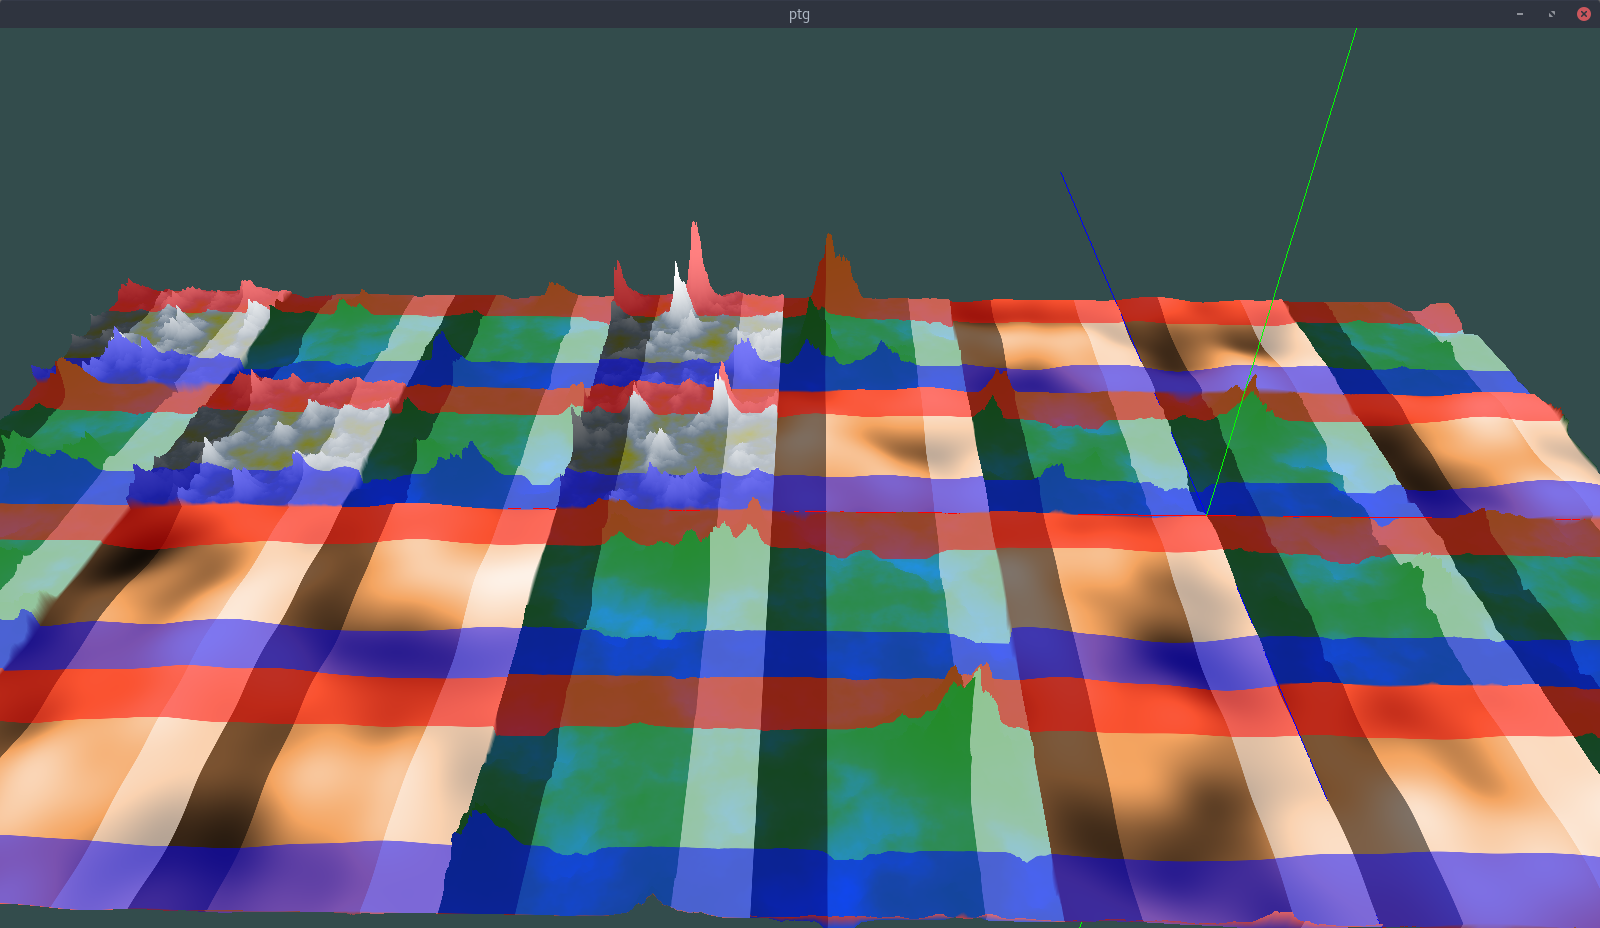
\includegraphics[width=0.48\textwidth]{figuras/border/l128.png}\label{fig:l128np}}\\
     \caption{Demarcação de fronteira.}
     
     \label{fig:borderlenanotherauxyeah}
     % usar \hspace{0.1cm}, é gambiarra mas funciona
\end{figure}

Se usarmos como peso a distância relativa em cada cordenada, substituindo a variámovel
$peso$ do algoritmo \ref{alg:borderColor} por $BH_{x}.pDist$ nas linhas $5$ e $8$, já
nas linhas $13$ e $16$ substitui $peso$ por $BH_{z}.pDist$, o restante dos parâmetros
da figura \ref{fig:borderlenanotherauxyeahp}, são os mesmos das imagens \ref{fig:borderlenanotherauxyeah}.

\begin{figure}[H]
     \centering
     \subfloat[][$l = 32$]{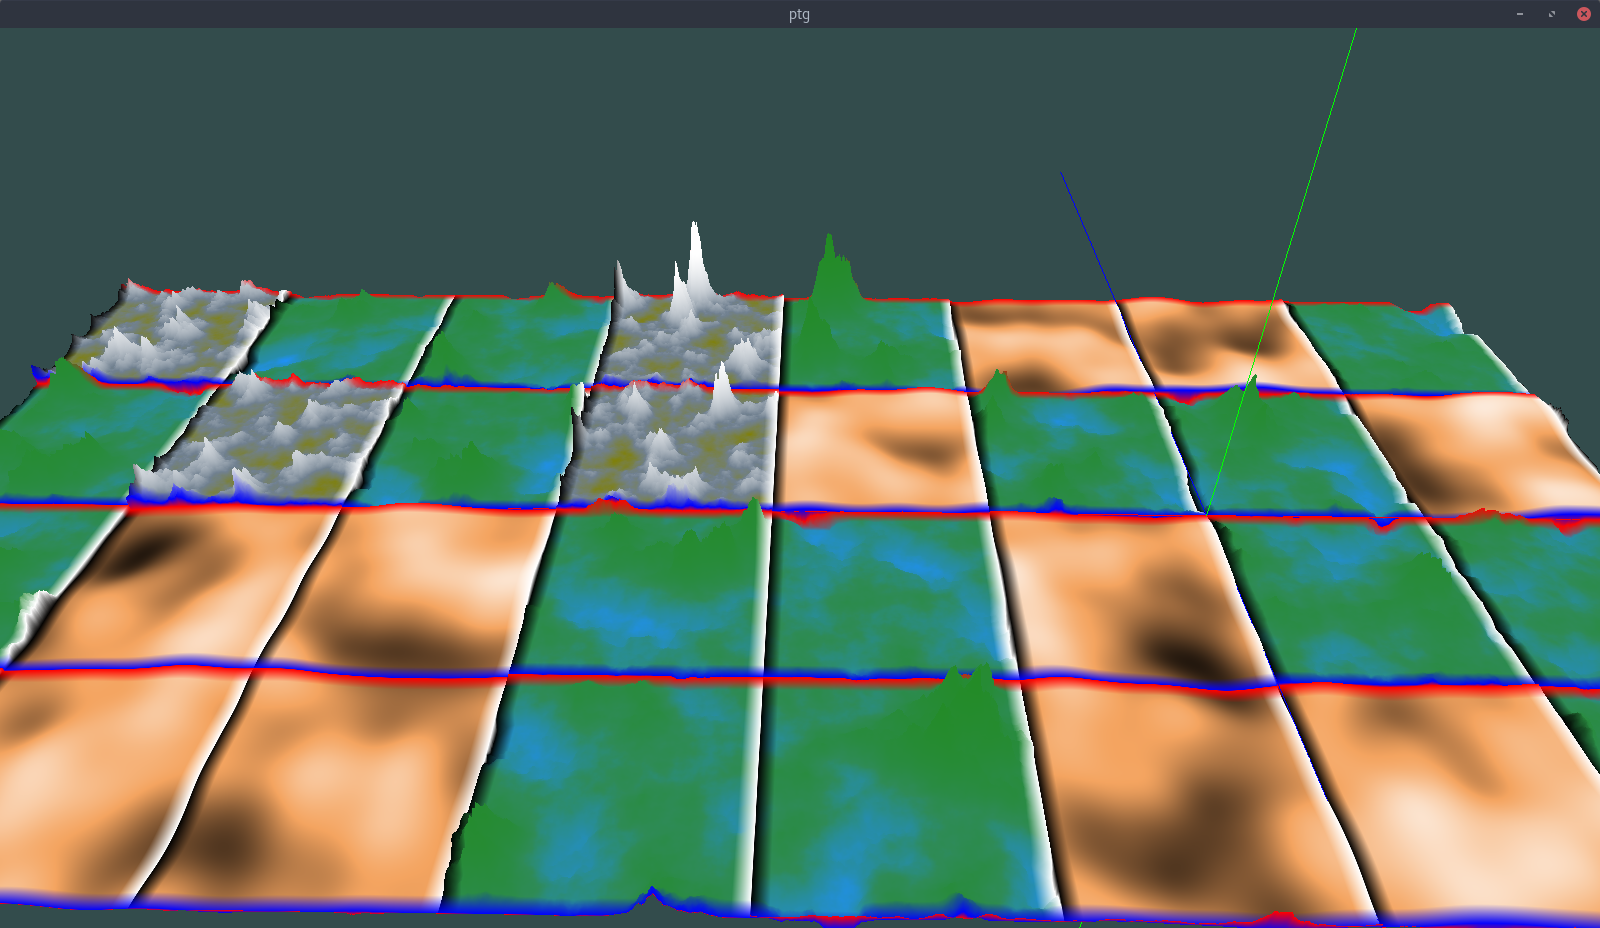
\includegraphics[width=0.48\textwidth]{figuras/border/l32p.png}\label{fig:l32p}}\hspace{0.1cm}
     \subfloat[][$l = 128$]{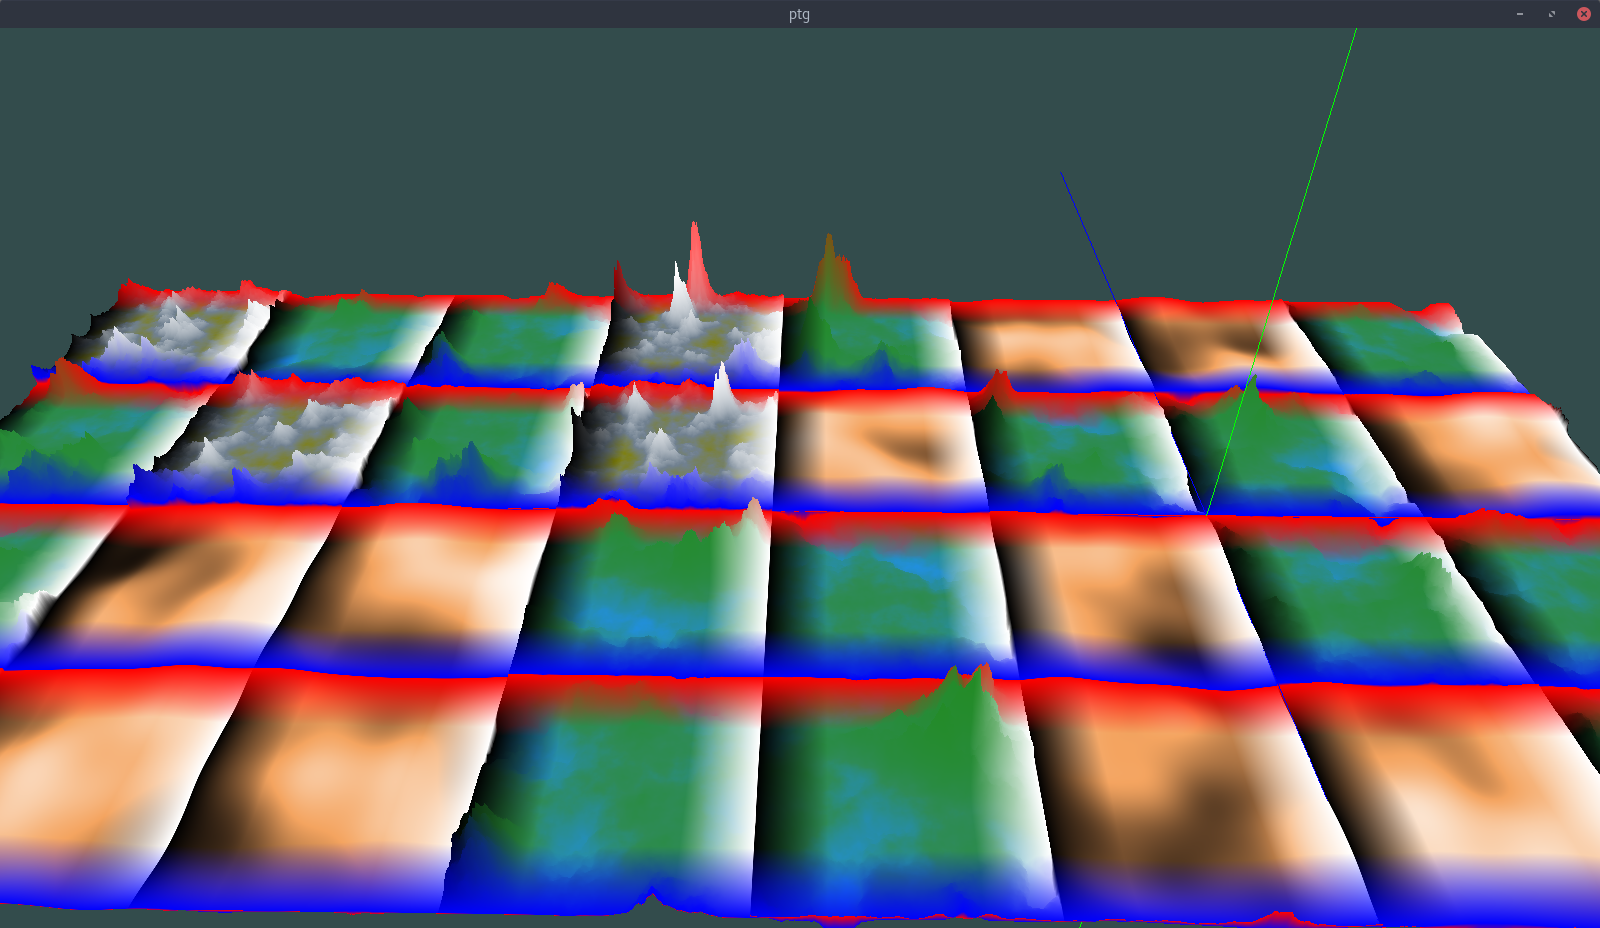
\includegraphics[width=0.48\textwidth]{figuras/border/l128p.png}\label{fig:l128p}}\\
     \caption{Demarcação de fronteira com peso na distância até a fronteira.}
     
     \label{fig:borderlenanotherauxyeahp}
     % usar \hspace{0.1cm}, é gambiarra mas funciona
\end{figure}

Desta maneira, cada área de bioma $(dxs, dzs)$ teria que ser responsável de fazer suavisação da 
fronteira com seus $8$ vizinhos 
$\{(dxs+1, dzs+1), (dxs+1, dzs), (dxs+1, dzs-1), (dxs, dzs+1), (dxs, dzs-1), (dxs-1, dzs+1), (dxs-1, dzs), (dxs-1, dzs-1)\}$
, é possivel fazer com que cada bioma faça suavisação com apenas 3 vizinhos, no caso do 
$(dxs, dzs)$, fará com $\{(dxs+1, dzs), (dxs, dzs+1), (dxs+1, dzs+1)\}$, assim cada 
bioma fará interpolação quando for sua flag $acimaFlag$ for verdadeira. Então
será o usado o algoritmo \ref{alg:borderColorr} e não o algoritmo \ref{alg:borderColor}.

\begin{algorithm}[H]\label{alg:borderColorr}%Usando parâmetro e não k
    $BH_{x} \leftarrow$ Algoritmo\ref{alg:borderTest}($x$)\;
    $BH_{z} \leftarrow$ Algoritmo\ref{alg:borderTest}($z$)\;
    
    \If {$BH_{x}.bordaFlag$}{
        \If {$BH_{x}.acimaFlag$}{
            $cor \leftarrow$ mix($(0, 0, 0)$, $cor$, $peso$)\;\tcc{Preto}
        }
    }
    \If {$BH_{z}.bordaFlag$}{
        \If {$BH_{z}.acimaFlag$}{
            $cor \leftarrow$ mix($(1, 0, 0)$, $cor$, $peso$)\;\tcc{Vermelho}
        }
    }
    
    \caption{Colorindo fronteira apenas acima.}
\end{algorithm}

\begin{figure}[H]
     \centering
     \subfloat[][Usando algoritmo \ref{alg:borderColor}]{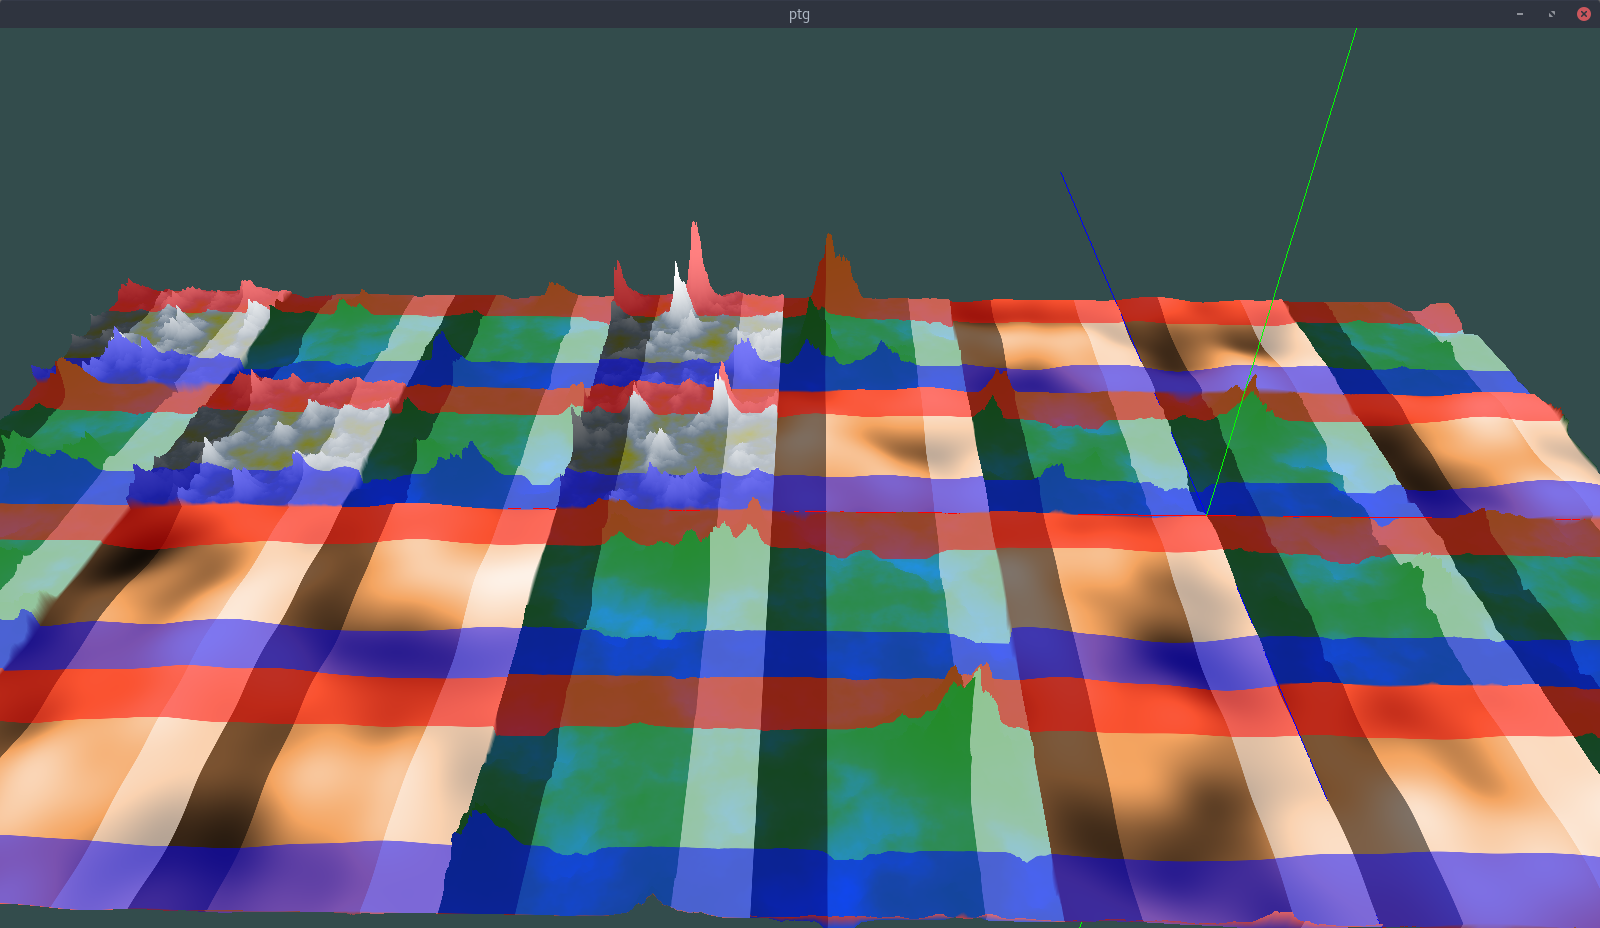
\includegraphics[width=0.48\textwidth]{figuras/border/l128.png}\label{fig:l32np666}}\hspace{0.1cm}
     \subfloat[][Usando algoritmo \ref{alg:borderColorr}]{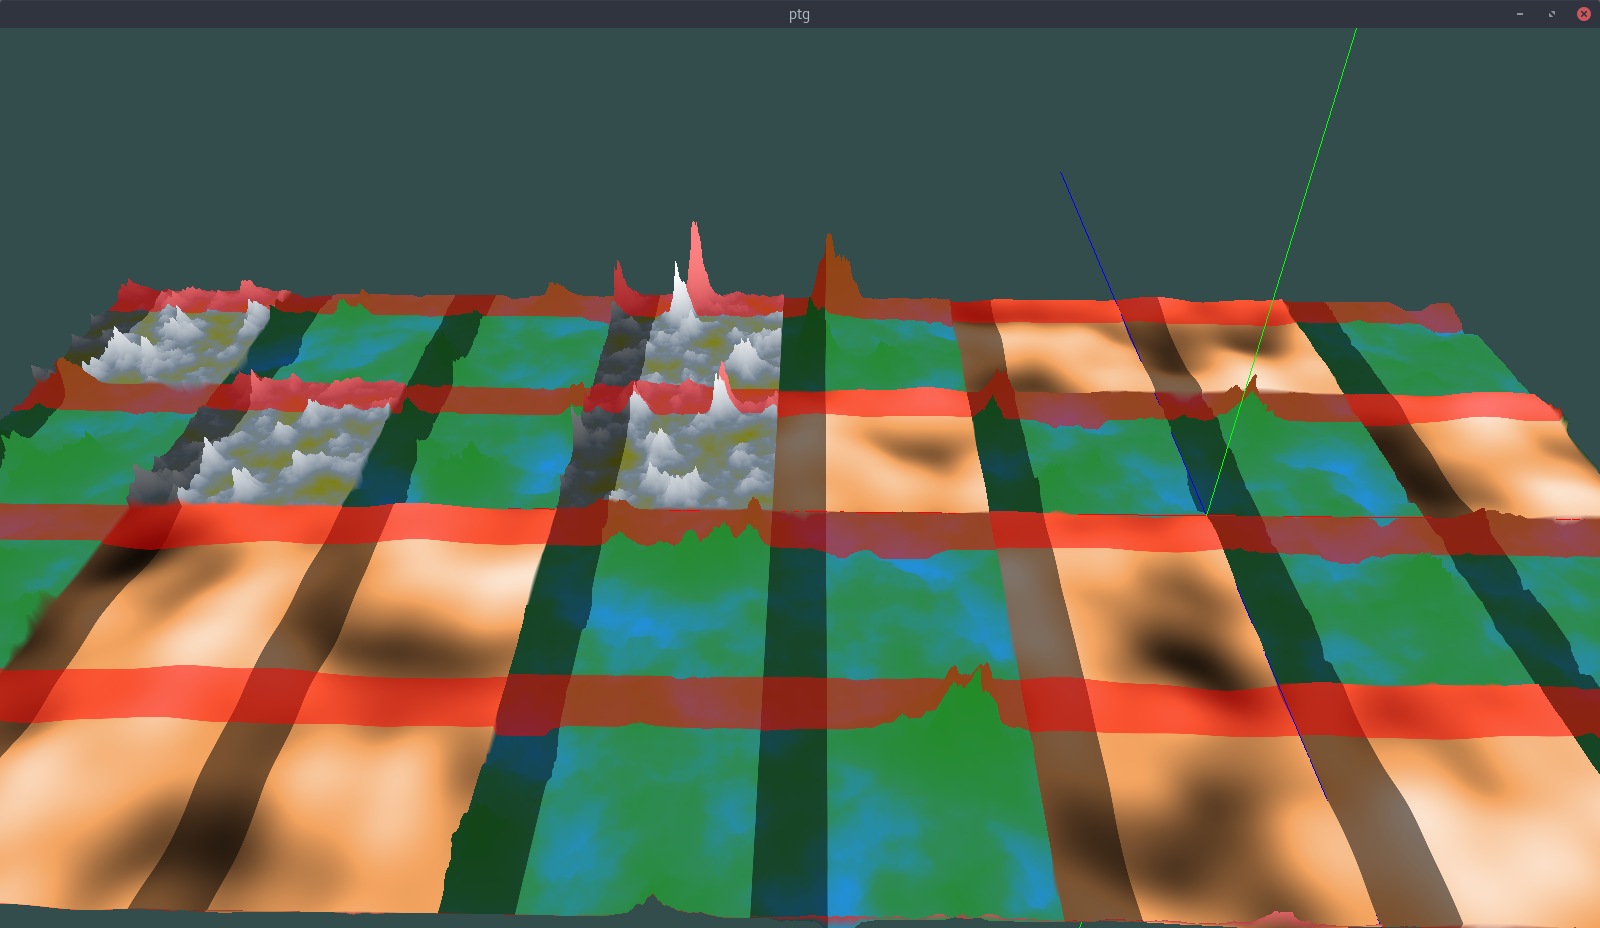
\includegraphics[width=0.48\textwidth]{figuras/border/l128aboveonly.png}\label{fig:l128aboveonly}}\\
     \caption{Comparando algoritmos com $l=128$.}
     
     \label{fig:borderlenanotherauxyeahaboveonly}
     % usar \hspace{0.1cm}, é gambiarra mas funciona
\end{figure}

Para suavizar as fronteriras é preciso saber quais valores de altura ($h$) e cor o
vértice que estamos calculando ($x, z$) teria se pertencesse ao bioma vizinho.

\begin{figure}[H]
    \centering
    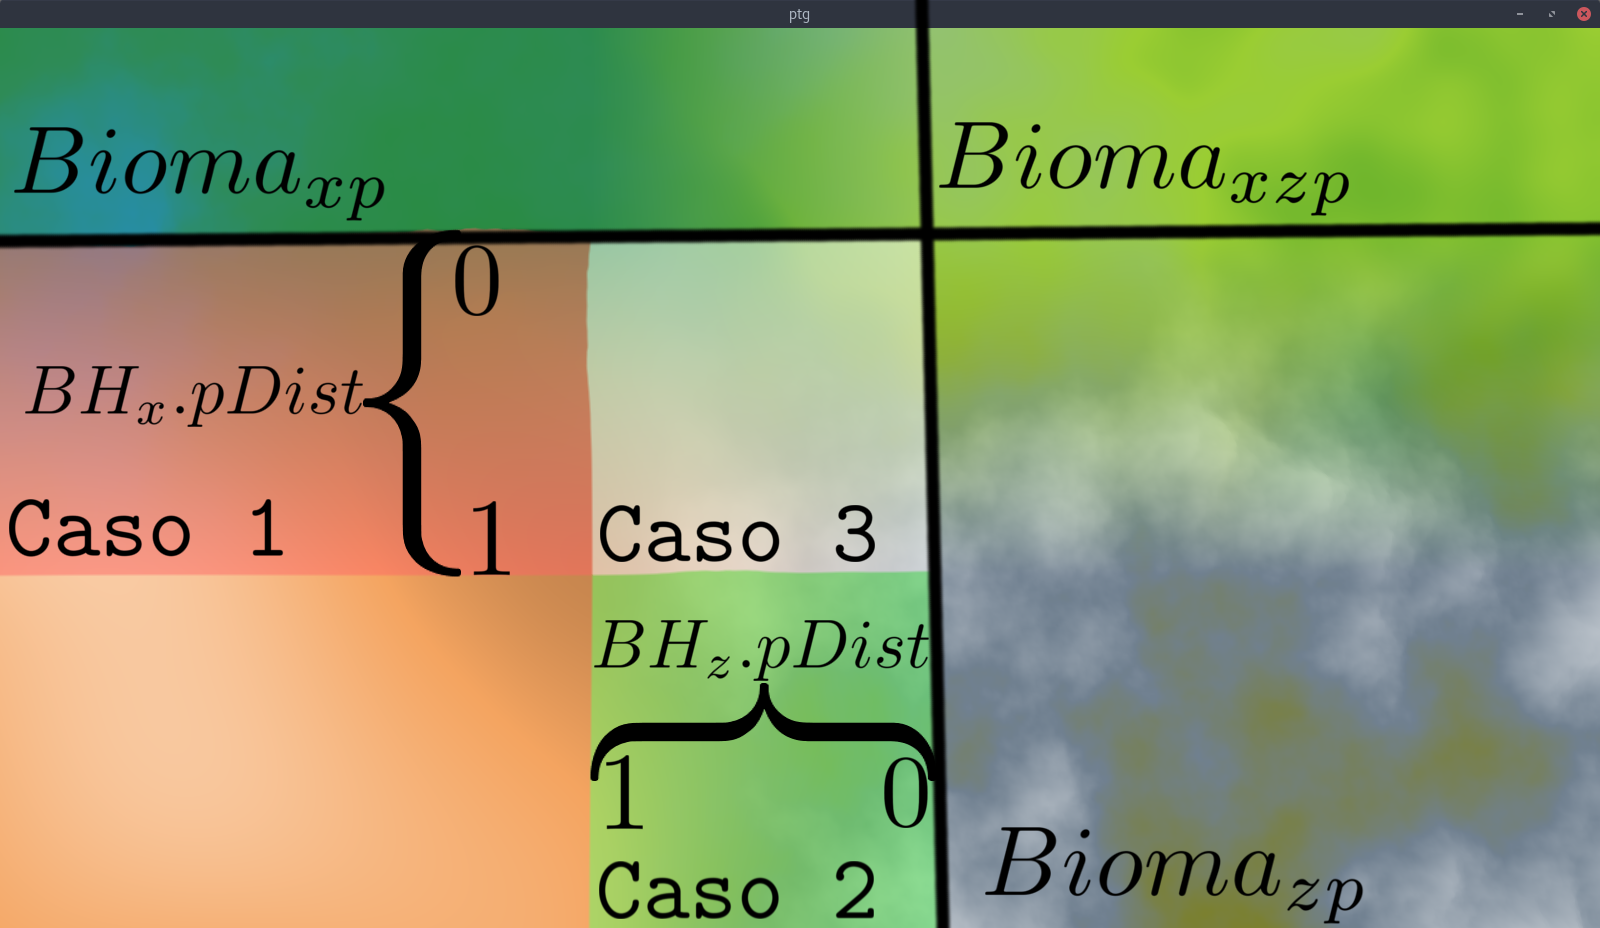
\includegraphics[width=0.75\textwidth]{figuras/border/yeah.png}
    \caption{Algumas variáveis do algoritmo \ref{alg:borderFinal}}
    \label{fig:paralgborder}
\end{figure}

\begin{algorithm}[H]\label{alg:borderFinal}%Usando parâmetro e não k
    $BH_{x} \leftarrow$ Algoritmo\ref{alg:borderTest}($x$)\;
    $BH_{z} \leftarrow$ Algoritmo\ref{alg:borderTest}($z$)\;
    $h_{p} \leftarrow h$\;
    $cor_{p} \leftarrow cor$\;
    \tcc{Caso1: $(x, z)$ é fronteira em $x$}
    \If {$BH_{x}.bordaFlag \land BH_{x}.acimaFlag$}{
        $Bioma_{xp} \leftarrow$ Algoritmo\ref{alg:getBiomeXZ}($x + l, z$)\;
        $afxz \leftarrow k/f_{Bioma_{xp}}$\;
        $h'_{xp} \leftarrow$ perlinNoise($x/afxz, z/afxz, \theta_{Bioma_{xp}}$)\;
        $h_{xp} \leftarrow$ Algoritmo\ref{alg:hBioValuation}($Bioma_{xp}$, $h'_{xp}$)\;
        $cor_{xp} \leftarrow$ Algoritmo\ref{alg:colorValuation}($minColor_{Bioma_{xp}}, midColor_{Bioma_{xp}}, maxColor_{Bioma_{xp}}, h'_{xp}$)\;
        $h \leftarrow$ mix($h_{xp}, h_{p}, BH_{x}.pDist$)\;
        $cor \leftarrow$  mix($cor_{xp}, cor_{p}, BH_{x}.pDist$)\;
    }
    \tcc{Caso2: $(x, z)$ é fronteira em $z$}
    \If {$BH_{z}.bordaFlag \land BH_{z}.acimaFlag$}{
        $Bioma_{zp} \leftarrow$ Algoritmo\ref{alg:getBiomeXZ}($x, z + l$)\;
        $afxz \leftarrow k/f_{Bioma_{zp}}$\;
        $h'_{zp} \leftarrow$ perlinNoise($x/afxz, z/afxz, \theta_{Bioma_{zp}}$)\;
        $h_{zp} \leftarrow$ Algoritmo\ref{alg:hBioValuation}($Bioma_{zp}$, $h'_{zp}$)\;
        $cor_{zp} \leftarrow$ Algoritmo\ref{alg:colorValuation}($minColor_{Bioma_{zp}}, midColor_{Bioma_{zp}}, maxColor_{Bioma_{zp}}, h'_{zp}$)\;
        $h \leftarrow$ mix($h_{zp}, h_{p}, BH_{z}.pDist$)\;
        $cor \leftarrow$  mix($cor_{zp}, cor_{p}, BH_{z}.pDist$)\;
    }
    \tcc{Caso 3: $(x, z)$ é fronteira em $x$ e $z$}
    \If {$BH_{z}.bordaFlag \land BH_{x}.bordaFlag \land BH_{z}.acimaFlag \land BH_{x}.acimaFlag$}{
        $Bioma_{xzp} \leftarrow$ Algoritmo\ref{alg:getBiomeXZ}($x + l, z + l$)\;
        $afxz \leftarrow k/f_{Bioma_{xzp}}$\;
        $h'_{xzp} \leftarrow$ perlinNoise($x/afxz, z/afxz, \theta_{Bioma_{xzp}}$)\;
        $h_{xzp} \leftarrow$ Algoritmo\ref{alg:hBioValuation}($Bioma_{xzp}$, $h'_{xzp}$)\;
        $cor_{xzp} \leftarrow$ Algoritmo\ref{alg:colorValuation}($minColor_{Bioma_{xzp}}, midColor_{Bioma_{xzp}}, maxColor_{Bioma_{xzp}}, h'_{xzp}$)\;
        $h_{i1} \leftarrow$ mix($h_{xzp}, h_{xp}, BH_{z}.pDist$)\;
        $cor_{i1} \leftarrow$ mix($cor_{xzp}, cor_{xp}, BH_{z}.pDist$)\;
        $h_{i2} \leftarrow$ mix($h_{zp}, h_{p}, BH_{z}.pDist$)\;
        $cor_{i2} \leftarrow$  mix($cor_{zp}, cor_{p}, BH_{z}.pDist$)\;
        $h \leftarrow$ mix($h_{i1}, h_{i2}, BH_{x}.pDist$)\;
        $cor \leftarrow$ mix($cor_{i1}, cor_{i2}, BH_{x}.pDist$)\;
    }
    
    \caption{Interpolação nas fronteiras.}
\end{algorithm}

\begin{figure}[H]
     \centering
     \subfloat[][Não usando algoritmo \ref{alg:borderFinal}] {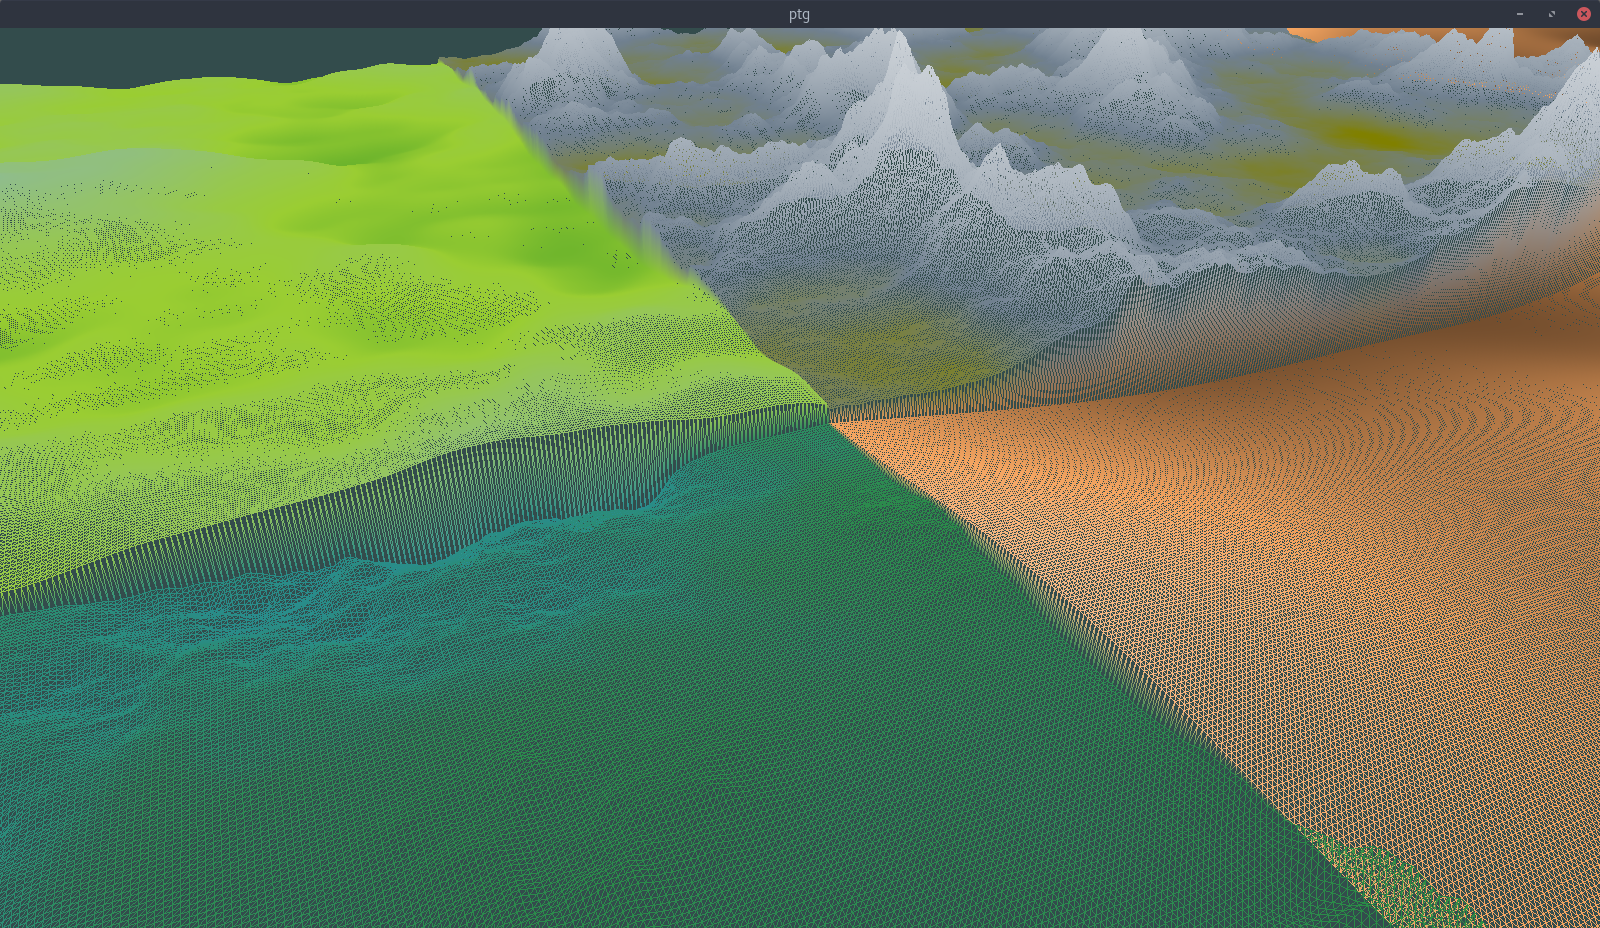
\includegraphics[width=0.48\textwidth]{figuras/border/a9/1s.png}\label{fig:nhaha1s}}\hspace{0.1cm}
     \subfloat[][Usando algoritmo \ref{alg:borderFinal}]{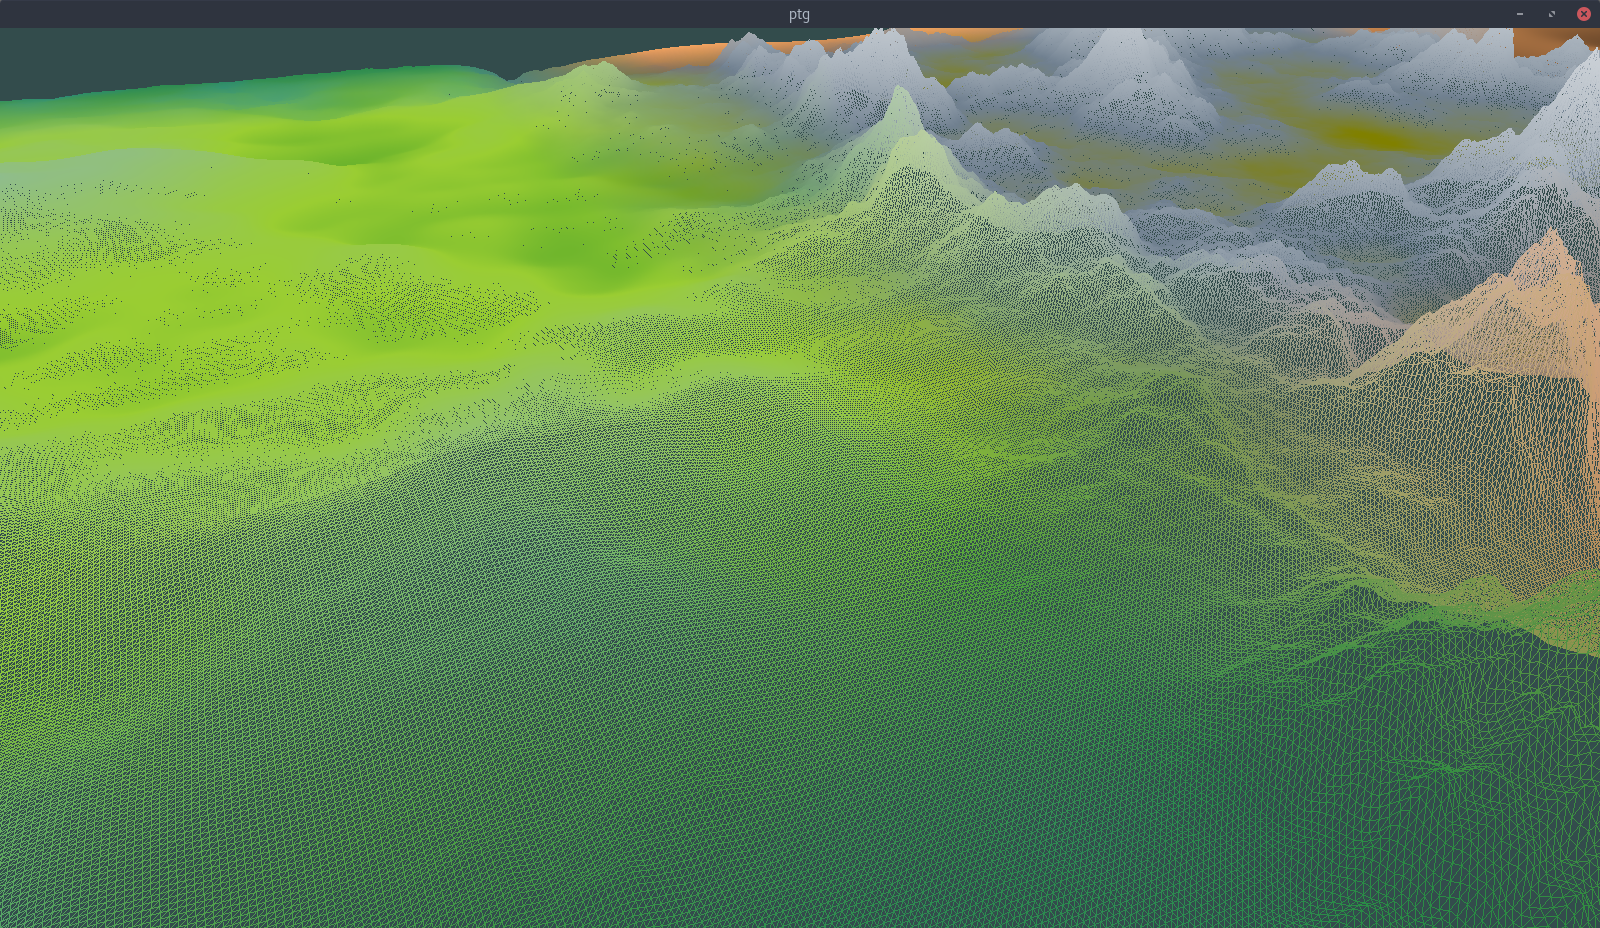
\includegraphics[width=0.48\textwidth]{figuras/border/a9/1c.png}\label{fig:nhaha1c}}\\
     \subfloat[][Não usando algoritmo \ref{alg:borderFinal}] {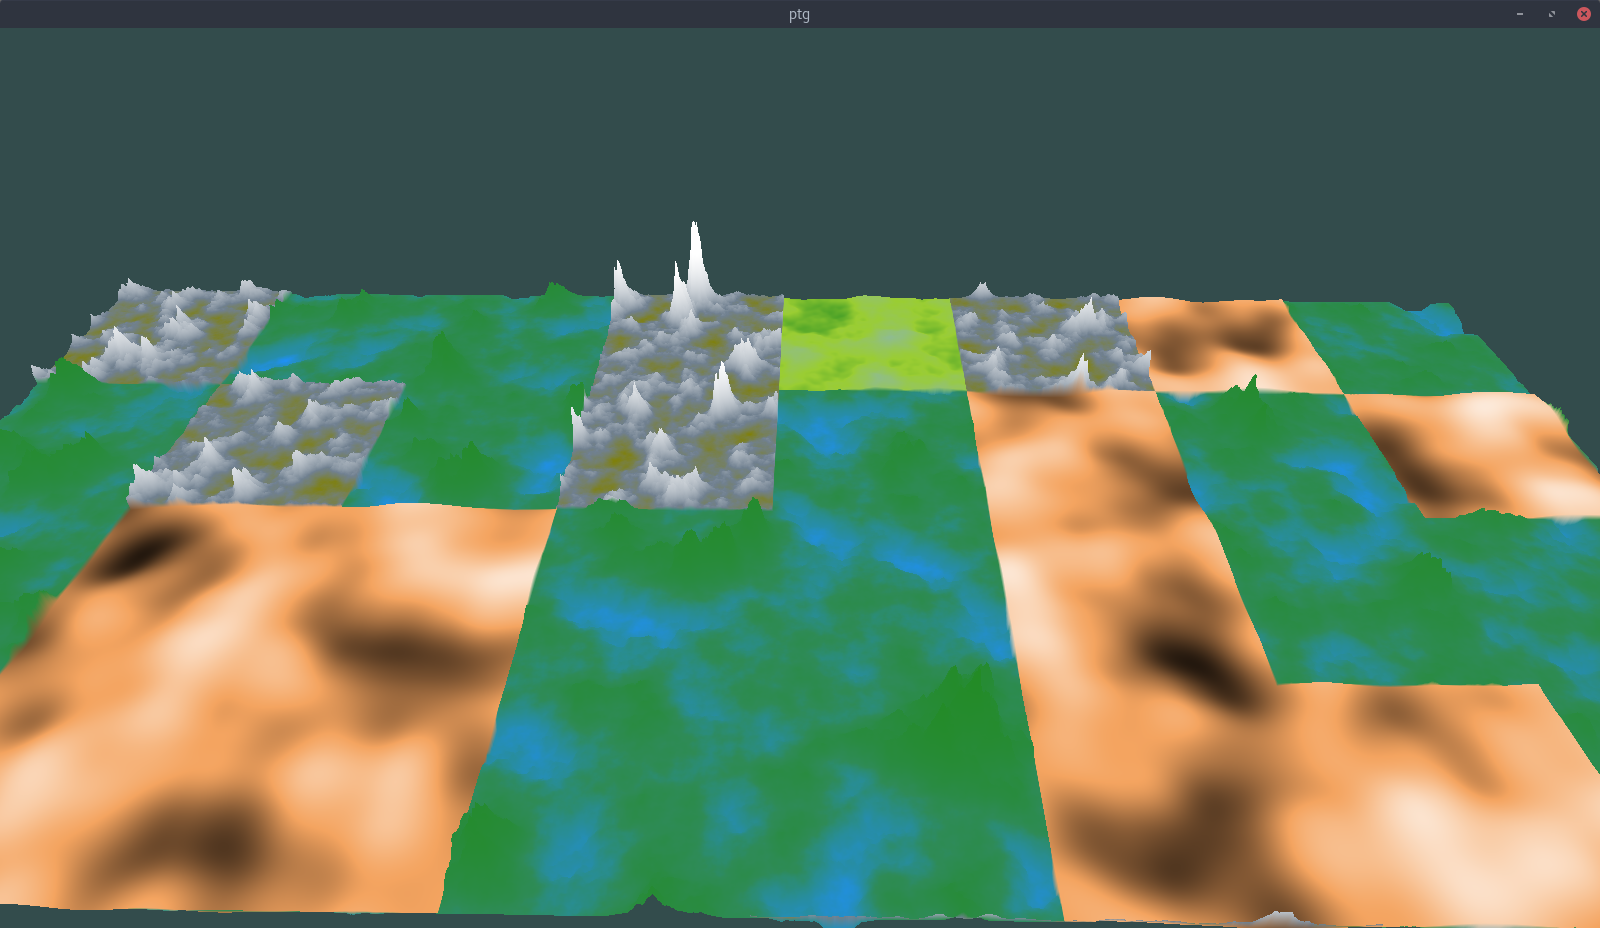
\includegraphics[width=0.48\textwidth]{figuras/border/a9/4s.png}\label{fig:nhaha4s}}\hspace{0.1cm}
     \subfloat[][Usando algoritmo \ref{alg:borderFinal}]{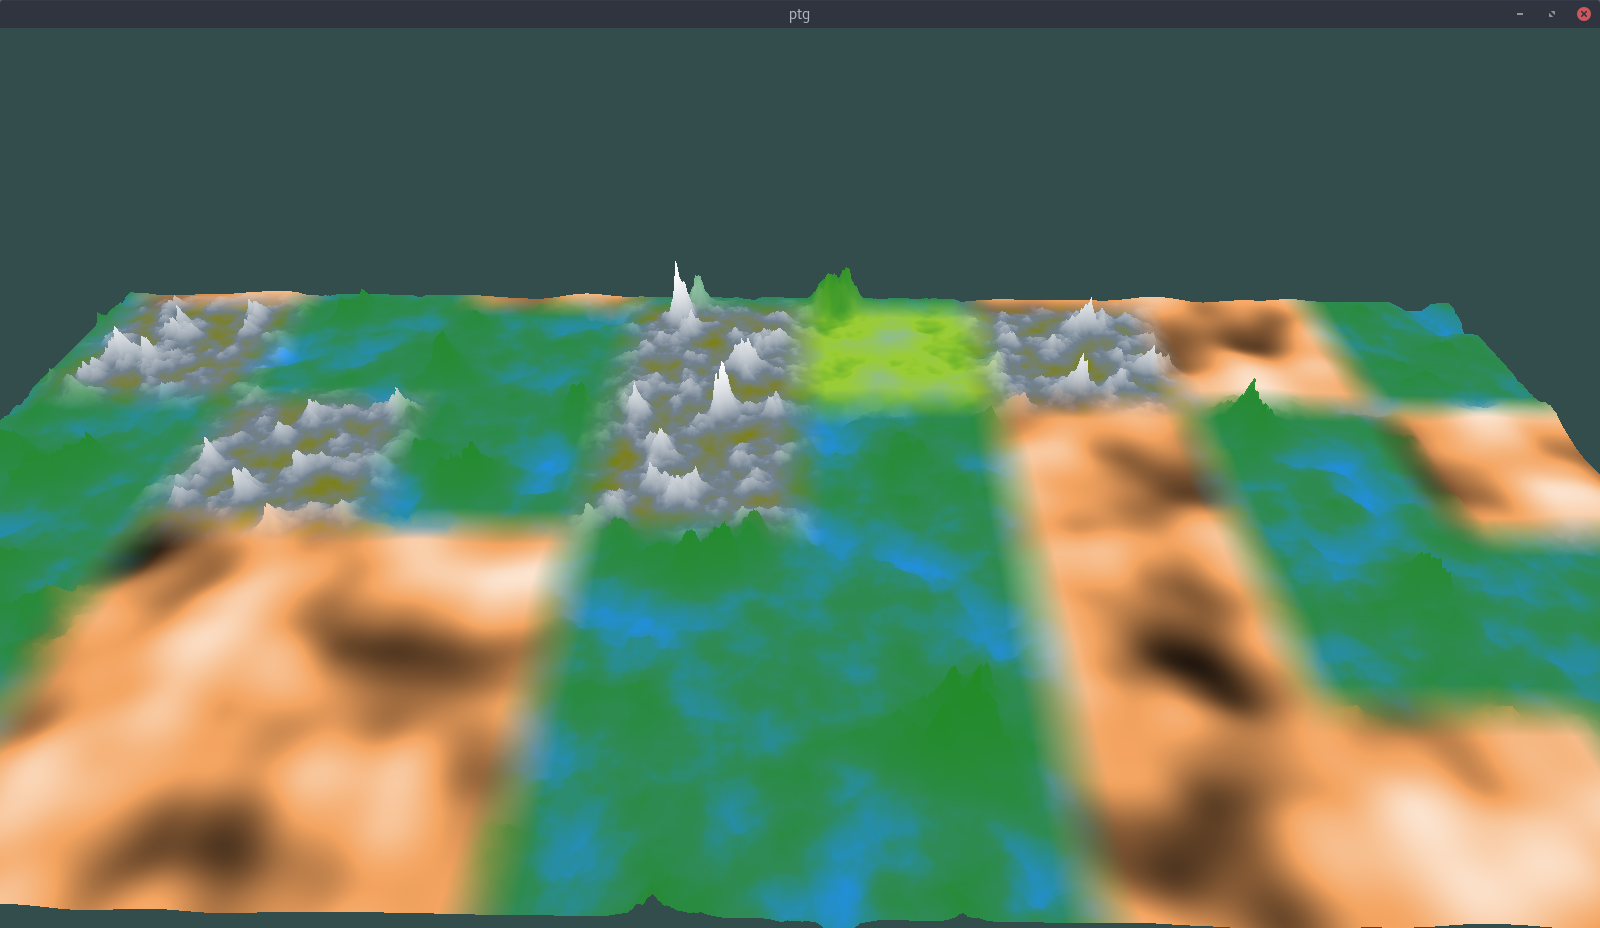
\includegraphics[width=0.48\textwidth]{figuras/border/a9/4c.png}\label{fig:nhaha4c}}\\
     \caption{Mostrando uso do algoritmo \ref{alg:borderFinal}.}
     
     \label{fig:a9usingandnot}
     % usar \hspace{0.1cm}, é gambiarra mas funciona
\end{figure}

\section{Valoração dos vértices}

Ainda resta juntar os alguns algoritmos em ordem...

\begin{algorithm}[H]\label{alg:vertexValuationm}%Usando parâmetro e não k
    \SetKwInOut{Input}{entrada}\SetKwInOut{Output}{output}
    \Input{$x \in \mathbb{Q}, z \in \mathbb{Q}$}
    $Bioma \leftarrow $Algoritmo\ref{alg:getBiomeXZ}($x, z$)\;
    $afxz \leftarrow k/f_{Bioma}$\;
    $h' \leftarrow$ perlinNoise($x/afxz, z/afxz, \theta_{Bioma}$)\;
    $cor \leftarrow$ Algoritmo\ref{alg:colorValuation}($minColor_{Bioma}, midColor_{Bioma}, maxColor_{Bioma}, h'$)\;
    $h \leftarrow$ Algoritmo\ref{alg:hBioValuation}($Bioma$, $h'$)\;
    Algoritmo\ref{alg:borderFinal}\;
    retorna $cor, h$\;
    \caption{Valoração de vértices.}
\end{algorithm}